\input{template/template}

\graphicspath{ {src/} }

\ifx\darkmode\undefined
\else
\pagecolor[rgb]{0.1569,0.1725,0.2039} %black
\color[rgb]{0.8275,0.8275,0.8275} %grey
\hypersetup{colorlinks,allcolors=}
\fi

\includeonly{
   src/acronyms,
   src/plan,
   src/introduction,
   src/background,
   src/literature_review,
   src/IPMI_implementation,
   src/config,
   src/Microstructure_eval,
   src/FRF_experiment,
   src/conclusions,
   src/future,
   src/publications,
   src/colophon,
 }



\newcommand{\titleinfo}{Generation of realistic white matter substrates with controllable morphology for diffusion MRI simulations}

\pagenumbering{Alph}
\begin{document}


%% Title Page
\author{Ross Callaghan}
\title{\titleinfo}
\supervisor{Main Supervisor}{Prof. Gary Zhang}
\supervisor{Co-Supervisor}{Dr. Marco Palombo}
\supervisor{Co-Supervisor}{Prof. Danny Alexander}
\thesisdate{\today}

%% Committee Page
\committeemember{President}{}{}
\committeemember{Referee}  {}{}
\committeemember{Referee}  {}{}
\committeemember{Referee}  {}{}




\maketitle
\pagestyle{empty}

% \ifx\finalversion\undefined
% \else
% \clearpage
% \begin{tikzpicture}[remember picture, overlay]
%   \node[anchor=center,inner sep=0pt] at (current page.center) {%
%     \includegraphics[width=\paperwidth]{wordcloud/wordcloud0.png}
%   };
% \end{tikzpicture}
% \clearpage
% \begin{tikzpicture}[remember picture, overlay]
%   \node[anchor=center,inner sep=0pt] at (current page.center) {%
%     \includegraphics[width=\paperwidth]{wordcloud/wordcloud1.png}
%   };
% \end{tikzpicture}
% \fi


% \renewenvironment{dedication}
% {
%   \pagestyle{empty}% no header and footer
%   \cleardoublepage
%   \begin{flushright}

%   \vspace*{\stretch{3}}% some space at the top
%   \itshape             % the text is in italics
%   \rmfamily
%   \Large
% }
% {%
%   \par % end the paragraph
%   \vspace{\stretch{1}} % space at bottom is three times that at the top
%   \end{flushright}
% }


% \begin{dedication}
%   To Charlie, my best friend and love of my life.
% \end{dedication}



\renewcommand*{\chapterpagestyle}{empty}
%\renewcommand{\BrainFuckChapter}{
%+}{+}{+}{+}{+}{+}{+}{+}{[}{>}{+}{+}{+}{+}{>}{+}{+}{+}{+}{+}{+}{>}{+}{+}{+}{+}{+}{+}{+}{+}{>}{+}{+}{+}{+}{+}{+}{+}{+}{+}{+}{>}{+}{+}{+}{+}{+}{+}{+}{+}{+}{+}{+}{+}{<}{<}{<}{<}{<}{-}{]}{>}{>}{>}{+}{.}{>}{>}{+}{+}
%{.}{+}{+}{+}{+}{+}{+}{+}{+}{+}{+}{+}{+}{+}{+}{+}{+}{+}{.}{+}{.}{-}{-}{.}{<}{+}{+}{+}{+}{+}{+}{+}{+}{+}{+}{+}{+}{+}{+}{+}{+}{+}{.}{+}{+}{.}{>}{+}{+}{.}{[}{>}{]}{<}{[}{[}{-}{]}{<}{]}{<}{<}{-}{<}{+}{+}{-}{<}{-}{-}
%}
\chapter*{Abstract}
%\addcontentsline{toc}{chapter}{Abstract}


Abstract goes here

%%% Local Variables:
%%% mode: latex
%%% TeX-master: "../main"
%%% End:

\renewcommand*{\chapterpagestyle}{plain}
\cleardoublepage
\pagestyle{plain}
\pagenumbering{roman}

\renewcommand{\BrainFuckChapter}{
}

\phantomsection
\addcontentsline{toc}{chapter}{Contents}

\tableofcontents

\renewcommand{\BrainFuckChapter}{
}
\listoffigures

\renewcommand{\BrainFuckChapter}{
}

\listofalgorithms
\addcontentsline{toc}{chapter}{List of Algorithms}



\chapter*{List of Acronyms}
\addcontentsline{toc}{chapter}{List of Acronyms}

\makeatletter
\patchcmd{\AC@@acro}{] #3}{] \MakeUppercase #3}{}{}
\patchcmd{\AC@@acro}{] #3}{] \MakeUppercase #3}{}{}
\makeatother
%%%%%%% ACRONYMS%%%%%%%%%%%
\begin{acronym}
  \acro{EA}[EA]{example acronym}
  \acro{UCL}[UCL]{University College London}
\end{acronym}


%%% Local Variables:
%%% mode: latex
%%% TeX-master: "../main"
%%% End:


\cleardoublepage

\acresetall{}
\renewcommand*{\chapterpagestyle}{scrheadings}

\pagestyle{scrheadings}
\pagenumbering{arabic}
% \chapter{Rough Plan	}
\label{sec:plan}

\section{General idea}
Summary of work done so far in PhD. That is, GPU diffusion simulations and fibre growth algorithm. 
The general 


\part{Introduction and background}
\label{part:intro_background}
\renewcommand{\LifeChapter}{y}
\chapter{Introduction}
\label{sec:introduction}

\chaptertoc{}

\begin{chapterabstract}
  This purpose of this chapter is to introduce the main motivations behind this project, from the historical relevance of \acl{dMRI} to the use of modern simulations for validating new \acl{dMRI} models.
  This chapter also sets out the problem that this project aims to address and the specific aims for addressing various aspects of it.
\end{chapterabstract}

\section{Motivation}
\label{sec:intro_motivation}
In 1992, James Watson, co-discoverer of DNA, said ``The brain is the last and grandest biological frontier, the most complex thing we have yet discovered in our universe.''\cite{NAP1785}.
One year later, Francis Crick, fellow discoverer of DNA, and Edward Jones published a commentary in Nature lamenting how little was understood about human neuroanatomy, saying that new techniques were needed beyond the contemporary tracer studies in non-human primates \cite{Crick1993}.\footnote{This introduction was inspired by Richard Passingham's very nice foreword to Diffusion MRI by Berg and Behrens \cite{Johansen-Berg2013}}

Just one year after that, in 1994, Basser et al.\ \cite{Basser1994} showed that it was possible to use \ac{MRI} to measure the movement of water along axons, providing the basis for exactly the kind of new technique Crick and Jones had felt was needed.
This technique of using \ac{MRI} for measuring the movement of water molecules is known as \ac{dMRI}.

In the 25 years since the work of Basser et al.\ the field of \acl{dMRI} has grown into a major topic of \ac{MRI} research, generating thousands of publications per year.
Diffusion MRI has found extensive use for imaging the brain, generating new techniques such as tractography which attempts to map out the connections in the brain \emph{in vivo}.
Another technique which takes advantage of \ac{dMRI} is microstructure imaging, in which measurements of the diffusion of water in tissue is used to infer information about the structure of the tissue. 

\begin{comment}
\ac{MRI} provides researchers and clinicians a powerful and flexible tool for non-invasively imaging the human body \emph{in vivo} and has found extensive use over the past few decades in furthering the understanding the structure and function of the human brain.
One technique which is commonly employed to study the structure of the human brain is \ac{dMRI}.
\end{comment}

These techniques work because \ac{dMRI} sensitises the \ac{MRI} signal to the diffusive motion of water molecules.
The environment in which the water molecules move will restrict the motion of the molecules and so will affect the \ac{MRI} signal. 
This dependency of the \ac{dMRI} signal on the environment in which water molecules diffuse can be exploited to infer information about the environment solely from the \ac{dMRI} signal.  
Microstructure imaging attempts to do exactly this, infer information about the microstructural environment such as cell size and density from the \ac{dMRI} signal.
In order to infer meaningful information from the \ac{dMRI} signal, models are typically used which relate microstructural features to the \ac{dMRI} signal.

The validation of these microstructural models can be difficult since ground truth microstructural features are typically inaccessible \emph{in vivo} and classical histological validation techniques have limitations such as disruption due to tissue extraction and preparation. 
One approach commonly taken for the validation of new models is simulation of the \ac{dMRI} signal using well defined and controllable ground truth microstructural environments known as numerical phantoms. 

Whilst these numerical phantoms often provide a valuable ground truth for simulation, they typically over simplify the complex microstructure of real tissue.
An example of this is in \ac{WM}, where fibres are commonly represented as straight cylinders \cite{Hall2009,Leemans2005} whereas in real tissue, fibres have complex shapes with undulation and diameter variation \cite{Nilsson2013,Lee2018a}.

In order to validate models in scenarios that are as close as possible to \emph{in vivo} conditions, the realism of numerical phantoms should be improved, attempting to fully capture all of the microstructural variation found in \emph{in vivo}.

Another application of numerical phantoms which is growing in popularity is in the direct computational modelling of microstructure.
These techniques use machine learning or fingerprinting-style techniques to match simulated signals and the corresponding ground truth microstructure of the numerical phantom to the measured signal \cite{Rensonnet2018,Hill2018,Palombo2018a,Nedjati-Gilani2017}.
Again, in this case, the more realistic the numerical phantoms used for simulation, the more accurately microstructural features can be estimated. 

With increased complexity of numerical phantoms, however, the computational cost of \ac{dMRI} simulations grows. Complex numerical phantoms are typically represented by polygon meshes and as the number of faces in a mesh grows, the computational cost of simulating the diffusion process grows.

In order to attempt to account for some of this increased computational complexity, adapting the \ac{dMRI} simulations for the \ac{GPU} can provide a performance boost.

The \ac{GPU} has a different architecture to the \ac{CPU}, being designed for parallel processing of graphics data.
Over the past decade, utilising the GPU for performing non-graphics calculations has become increasingly popular. 
In short, the goal is to exploit the parallel design of the \ac{GPU} to perform  many calculations simultaneously.
There are certain limitations on the kind of tasks that can be improved by the \ac{GPU}, for instance, as a minimum the problem must be parallelisable.
\ac{dMRI} simulations are inherently parallel, meaning that adapting the simulations for \ac{GPU} should be able to bring a performance increase. 

\section{Problem Statement}
\label{sec:intro_problem_statement}
There is a need to be able to generate numerical phantoms that realistically represent \ac{WM} microstructure, with controllable microstructural parameters such as axon packing density and orientation dispersion, and to improve the efficiency of \ac{dMRI} simulations.


\section{Project Aims and Scope}
\label{sec:intro_project_aims}
This report summarises work towards improving the realism of simulations of diffusion \ac{MRI}. Realistic simulations allow models of the MRI signal to be validated using controllable and well known ground truth.

 

The mains aims of this work are as follows:
% \begin{itemize}
% \item Present \acused{ConFiG} \acs{ConFiG} (\textbf{Con}textual \textbf{Fi}bre \textbf{G}rowth), a method developed for `growing' fibres densely while attempting to respect some morphological priors to generate realistic \ac{WM} numerical phantoms.
% \item Present CUDAmino, a \ac{GPU} accelerated \ac{MC} \ac{dMRI} simulator based on the \ac{MC} simulation in Camino\cite{Cook2006,Hall2009}
% \end{itemize}
\begin{enumerate}
\item Develop and test a method for generating realistic \ac{WM} numerical phantoms with realistic and controllable axon packing densities and orientation dispersion
\item Develop and test a \ac{GPU} accelerated \ac{dMRI} simulator
\end{enumerate}

In an effort to achieve aim 1, a method called\acused{ConFiG} \acs{ConFiG} (\textbf{Con}textual \textbf{Fi}bre \textbf{G}rowth) is presented which `grows' fibres densely attempting to respect some morphological priors to generate realistic \ac{WM} numerical phantoms.
%\ac{ConFiG} is tested, using it to general phantoms with simple morphology that can be easily generated using other means to test its ability to replicate simple situations and explore the input parameter space.


Additionally, to tackle aim 2, CUDAmino, a \ac{GPU} implementation of \ac{MC} \ac{dMRI} simulations is presented. The \ac{GPU} simulations are based on the \ac{MC} simulator software in Camino \cite{Cook2006,Hall2009} and leverage NVIDIA's \acs{CUDA} parallel programming platform \cite{Nickolls2008}.




\section{Report Overview}
\label{sec:intro_report_overview}
The rest of the report is arranged as follows: \Cref{sec:background} outlines some of the physics behind \acl{dMRI} and how we simulate it as well as some background on \ac{GPU} architecture and considerations for programming the \ac{GPU}. \Cref{sec:literature_review} reviews current literature on \ac{dMRI} simulations (including \ac{GPU} \ac{dMRI} simulations). \Cref{sec:config} outlines \ac{ConFiG} for generating new phantoms and some experiments assessing the performance of \ac{ConFiG} in some simple situations and presenting examples of realistic substrates. \Cref{sec:cudamino} presents CUDAmino and some experiments assessing its performance against the \ac{CPU} simulations. \Cref{sec:future} discusses future perspectives for the work.



%%% Local Variables:
%%% mode: latex
%%% TeX-master: "../main"
%%% End:

\renewcommand{\BrainFuckChapter}{y}
\renewcommand{\LifeChapter}{y}
\chapter{Background}
\label{chap:background}
\chaptertoc{}

\begin{chapterabstract}
  This chapter introduces the physics behind \ac{dMRI} as well as some techniques used for the simulation of \ac{dMRI}.
  Firstly, general MR physics is introduced building up from a single proton to the generation of the spin echo signal.
  The second section discusses how the diffusion of water molecules impacts the MR signal, leading to the diffusion signal attenuation.
  The third section introduces some simulation approaches which can be used to generate synthetic \ac{dMRI} data and the final section discusses the \ac{GPU} and how it may be used to accelerate \ac{dMRI} simulations. 
\end{chapterabstract}

\section{MR Physics}
\label{sec:bg_mri_physics}
All forms of \emph{in vivo} use of magnetic resonance have their origins in the 1940s when Purcell, Torrey and Pound independently and almost simultaneously with Bloch, Hansen and Packard detected radio frequency signals from nuclei in ordinary matter\cite{Levitt2008, Barker2009,Bloch1946,Purcell1946}.
This discovery gave birth to the field of \ac{NMR} which has become widespread, with applications in a number of areas including chemistry, biology, materials science and medical imaging\cite{Barker2009, Salibi1998}.

Within the medical imaging context, \ac{NMR} typically finds two uses, \acf{MRI} and \ac{MRS}\footnote{The `N' from NMR is dropped in the medical imaging context to avoid confusion with nuclear medicine and general squeamishness around the word nuclear}.
Both of these uses are closely related: \ac{MRI} is typically concerned with building images of internal structures in the body, whilst \ac{MRS} is concerned with identifying the chemical composition of tissues in the body.

The theory behind \ac{NMR} concerns the interaction between nuclei and magnetic fields. This section briefly introduces the \ac{NMR} physics relevant to \ac{dMRI}.

\subsection{Nuclear Magnetism}
\label{sec:bg_nuclearmagnetism}

The most important property of a nucleus for the application of \ac{NMR} is nuclear spin. 
Spin is a property inherent to all subatomic particles and whilst it is a purely quantum effect, it can be thought of loosely as the particle spinning around its axis - much like a tiny planet \cite{Levitt2008}.
A planet spinning about its axis will have an angular momentum associated with that rotation and similarly the spin of a particle behaves like an angular momentum.
Unlike the angular momentum of a rotating planet, however, the spin is an intrinsic property of the particle itself and not a result of its motion\cite{Levitt2008}.

\begin{comment}
One of the postulates of quantum mechanics is that angular momentum is quantised \cite{DeGraaf2007}. This means that the spin angular momentum, $S$, of a particle in its rest state can only take values of
\begin{equation}
S = \hbar \sqrt{(I(I+1))} \,,
\label{eq:angmom_quant}
\end{equation} 
where $I$ is the spin angular momentum quantum number which can only take integer or half-integer values and $\hbar$ is the reduced Planck constant \cite{DeGraaf2007}.
A second quantum number is used to describe the direction of angular momentum relative to a given direction, usually referred to as $z$. 
Again, this quantum number is quantised, with the angular momentum in the $z$ direction, $S_z$, given by 
\begin{equation}
S_z = \hbar m_z \,.
\label{eq:angmom_z}
\end{equation} 
The $m_z$ quantum number can have $2I + 1$ values in the range \cite{DeGraaf2007}
\begin{equation}
m_z = -I,\, -I + 1,\,\dots,\, I-1,\, I\,.
\label{eq:m_z}
\end{equation}

Protons, neutrons and electrons - the particles making up all everyday matter - all have a spin quantum number of $I = \sfrac{1}{2}$ meaning that $m_z$ can have two possible values $m_z = \pm \sfrac{1}{2}$.


% \todo{IS THIS BIT NECESSARY? JUST FOCUS ON PROTONS?}
% Nuclei are made up of protons and neutrons, so the spin of a nucleus will be given by the combination of the spins of the protons and neutrons in the nucleus.
% In general in quantum mechanics, the combination of two angular momenta will result in a third angular momentum, which can take a range of values according to 
% \begin{equation}
% I_{12} = |I_1 - I_2|, |I_1-I_2| + 1, \dots, |I_1 + I_2| - 1, |I_1 + I_2|\,. 
% \end{equation}
 
% The precise way in which the spins combine in any given nucleus is a complicated quantum mechanical problem but there are some rules which describe the possible nuclear spin quantum numbers. 
% A nucleus with an odd mass number will have a half-integer spin, a nucleus with even mass number and even atomic number will have zero spin and a nucleus with an even mass number and odd atomic number will have integer spin \cite{DeGraaf2007}.

This project is focused on \ac{NMR} of \ce{^1H} nuclei in water molecules, which simply consist of a single proton and so have $I = \sfrac{1}{2}$. 
\ac{NMR} is, however, feasible on any nucleus with non-zero spin with some of the most biologically relevant nuclei for in-vivo MRS being \ce{^{13}C}, \ce{^{31}P} and \ce{^{23}Na} \cite{DeGraaf2007}.
\end{comment}


\ac{MRI} typically relies on \ac{NMR} of \ce{^1H} nuclei in water molecules, which simply consist of a single proton.
A proton carries a positive electric charge.
Just as classically a rotating charge with angular momentum, $\mathbf{L}$, will produce a magnetic moment, $
\boldsymbol{\mu} = \gamma \mathbf{L}$, the intrinsic spin angular momentum, $\mathbf{S}$ of a proton will produce a magnetic moment 
\begin{equation}
\label{eq:magnmom}
\boldsymbol{\mu} = \gamma \mathbf{S} \,,
\end{equation}
where $\gamma$ is the gyromagnetic ratio \cite{Levitt2008}.
For a proton, $\gamma = 2.675 \times 10^8$ rad s$^{-1}$ T$^{-1}$.

The fact that a proton has an intrinsic magnetic moment means that it will interact with magnetic fields and it is understanding this interaction that underpins \ac{NMR} theory.


\subsection{Magnetic Resonance}
\label{sec:bg_resonance}
Classically, a magnetic moment, $\boldsymbol{\mu}$, placed in an external magnetic field, $\mathbf{B}_0$, will feel a torque, $\boldsymbol{\tau}$, given by \cite{Haacke1999} 
\begin{equation}
\label{eq:torque}
\boldsymbol{\tau} = \boldsymbol{\mu} \times \mathbf{B}_0 \,.
\end{equation}
At the same time, classical mechanics gives a relationship between the change in angular momentum and the torque as \cite{Haacke1999} 
\begin{equation}
\label{eq:dLdt}
\frac{d\mathbf{L}}{dt} = \boldsymbol{\tau}\,. 
\end{equation}
For a proton in its rest state, the only angular momentum is the intrinsic spin angular momentum, $\mathbf{S}$, so combining \Cref{eq:torque,eq:dLdt} gives the equation of motion for a spin in an external magnetic field
\begin{equation}
\frac{d\mathbf{S}}{dt} = \boldsymbol{\mu} \times \mathbf{B}_0 \,.
\end{equation}
Since $\mathbf{S}$ is equivalent to $\boldsymbol{\mu}/\gamma$ (\Cref{eq:magnmom}), this becomes
\begin{equation}
\frac{d\boldsymbol{\mu}}{dt} = \gamma\boldsymbol{\mu} \times \mathbf{B}_0\,.
\label{eq:dmudt}
\end{equation}

This equation of motion can be solved in a few ways for the case of constant external magnetic field, with the result being that the magnetic moment precesses about the magnetic field with a frequency, $\omega_0$, given by\cite{Levitt2008}
\begin{equation}
\label{eq:LarmorFreq}
\omega_0 = \gamma B_0\,,
\end{equation}
with $B_0$ being the external field strength. 
This precessional motional is illustrated in \Cref{fig:precession}.
The frequency $\omega_0$ is known as the Larmor frequency and lies in the \ac{RF} range for typical field strengths found in MRI machines (1.5 - 7 T).

\begin{figure}
	\centering
	\begin{subfigure}{0.3\textwidth}
		\includegraphics[width = \textwidth]{figures/background/precession.eps}
		\caption{}
		\label{fig:precession}
	\end{subfigure}
	\hspace{2cm}
	\begin{subfigure}{0.3\textwidth}
		\includegraphics[width = \textwidth]{figures/background/manyspins.eps}
		\caption{}
		\label{fig:manyspins}
	\end{subfigure}
	
	\caption[Illustration of the precessional motion of a single spin and production of magnetisation by many spins]{a) Illustration of the precessional motion of a single spin with magnetic moment $\mu$ in the presence of an external magnetic field $B_0$. b) Many individual spins in an external magnetic field precess around the external field with random phase producing a net magnetisation in the direction of the $B_0$ field.}
	\label{fig:precession-spins}
	
\end{figure}


In practice, it is not possible to observe the magnetic moment of a single spin. 
The quantity observed is rather the sum of the magnetic moments from many spins together, this is known as the net magnetisation. 
%In order to fully describe the system, a quantum mechanical treatment using density operators is necessary \cite{Levitt2008}, however a classical treatment is sufficient to understand the basic principles.

\begin{comment}
As mentioned in \Cref{sec:bg_nuclearmagnetism}, protons can have two $S_z$ states with $m_z = \pm \sfrac{1}{2}$. 
These states can be thought of as the magnetic moment either being aligned parallel or anti-parallel to the external magnetic field, known as spin-up and spin-down respectively.

\begin{figure}
	\centering
	\includegraphics[width=0.6\textwidth]{figures/background/energy_levels.eps}
	\caption{Energy levels of a spin-1/2 particle. The spin-up state ($\alpha$) has the lowest energy and the spin down state ($\beta$) has the highest. The energy difference between the levels is $\Delta E$.}
	\label{fig:energylevels}
\end{figure}

The energy difference between these two states is given by a quantum mechanical effect called the Zeeman effect \cite{Levitt2008}, which gives the difference as  
\begin{equation}
	\Delta E = \gamma \hbar B_0\,.
\end{equation} 

\Cref{fig:energylevels} illustrates this splitting of the energy levels showing that the spin-up state, $\alpha$, is the lower of the two energy states. 
When there are many protons all experiencing the same magnetic field, the proportion of the number of protons in the spin-up, $n_\alpha$, state versus spin-down, $n_\beta$, is given by the Boltzmann distribution\cite{DeGraaf2007}
\begin{equation}
\frac{n_\alpha}{n_\beta} = \exp\left(\frac{\Delta E}{k_BT}\right)\,,
\end{equation}  
where $k_B$ is the Boltzmann constant and $T$ is the temperature. This means that at a non-zero temperature and with positive $\gamma$, there are slightly more protons aligned with the magnetic field than against it.  
\end{comment}


In a sample, slightly more protons will align with the $\mathbf{B}_0$ field than against it, meaning that the net magnetisation will be parallel to $\mathbf{B}_0$. 
\Cref{fig:manyspins} shows a pictorial representation of the system of many spins producing a net magnetisation, $\mathbf{M}_0$ aligned with $\mathbf{B}_0$.

Each of the spins will still be precessing about the magnetic field at the Larmor frequency but since they are out of phase with one another, all transverse components of the magnetisation cancel out when they combine and all that is left is a static longitudinal component. 


In order to make measurements, the net longitudinal magnetisation needs to be `flipped' into the transverse plane where it can be detected. 
This is achieved by applying a second magnetic field, $\mathbf{B}_1$, oscillating in the transverse plane. 
In much the same way as with $\mathbf{B}_0$, the magnetisation feels a torque from $\mathbf{B}_1$ and begins to rotate about $\mathbf{B}_1$, away from the longitudinal axis.
The two external fields act simultaneously on $\mathbf{M}_0$ so the magnetisation will tip away from the $z$ axis whilst still precessing about $z$ with a frequency $\omega_0$.
This kind of motion is known as nutation and is illustrated in \Cref{fig:nutation}.

\begin{figure}
	\centering
	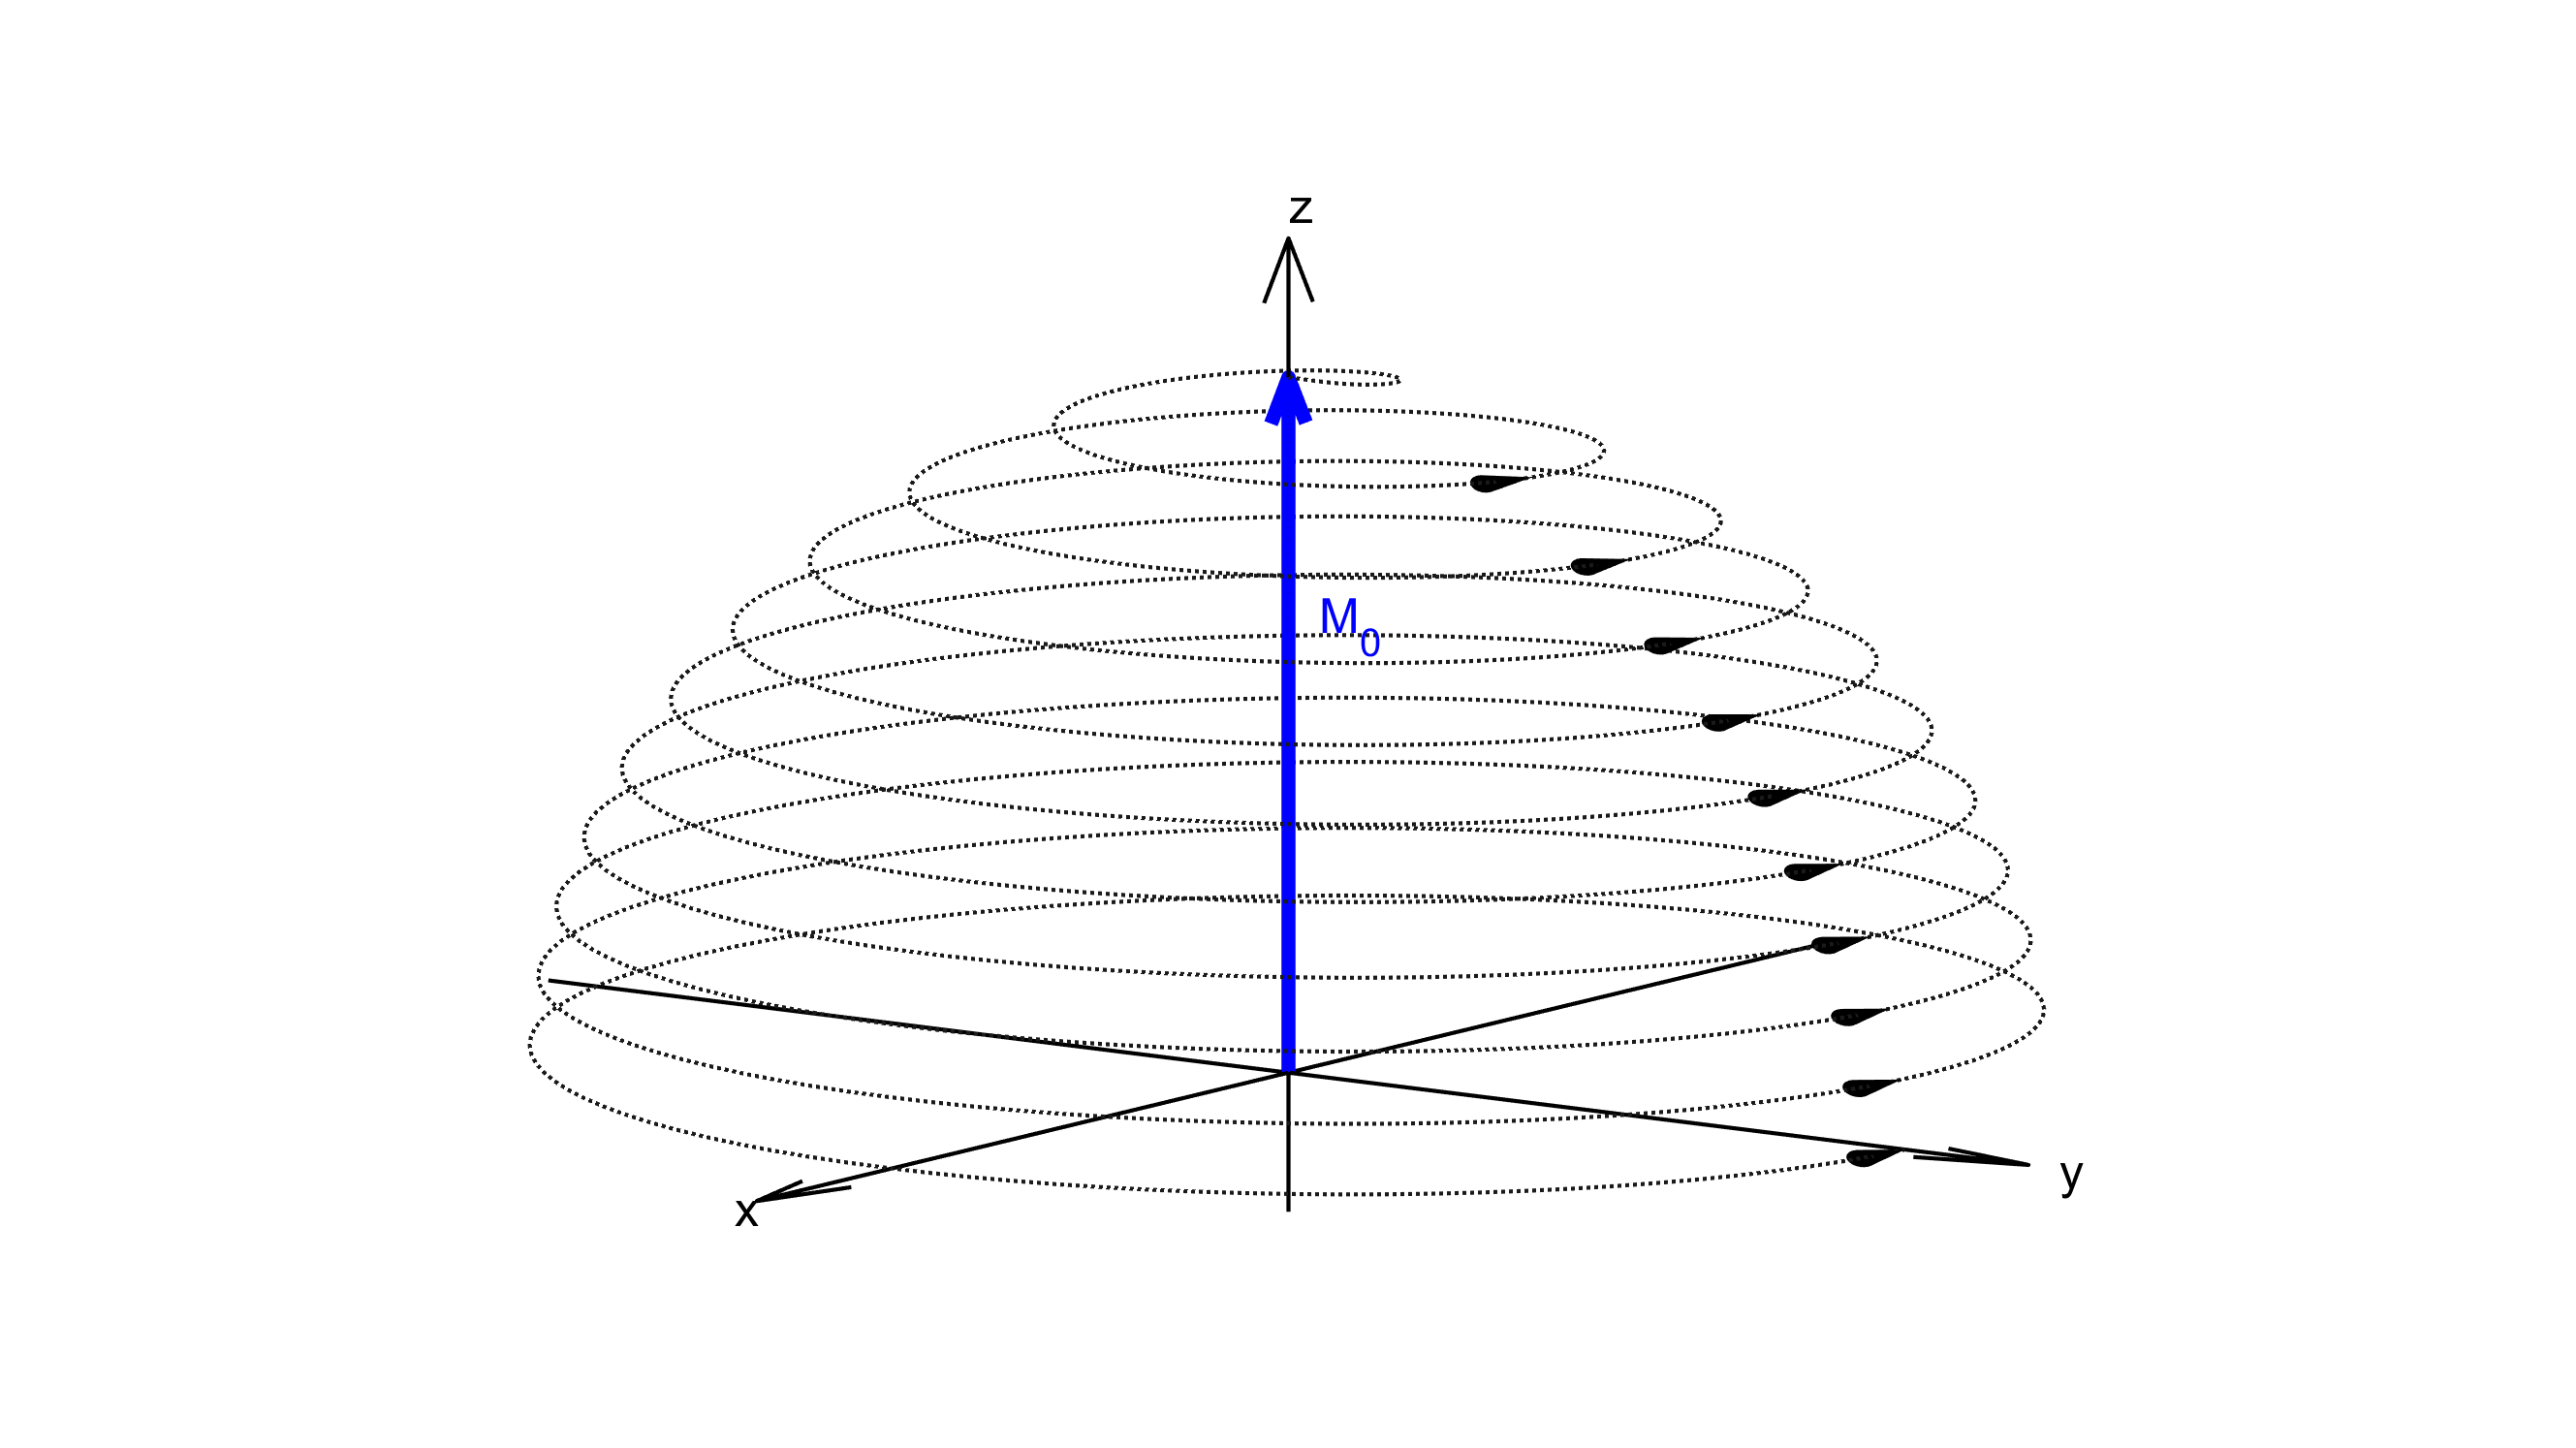
\includegraphics[width=\textwidth]{figures/background/nutation.eps}
	\caption[Nutation motion of an on-resonance spin the presence of an \ac{RF} field.]{Nutation motion of an on-resonance spin in the presence of an \ac{RF} field. Precession about the $B_0$ and $B_1$ fields create the spiralling motion in the laboratory frame.}
	\label{fig:nutation}
\end{figure}



\subsection{The Bloch Equations}
\label{sec:bg_bloch}
The interaction between the magnetisation and magnetic fields is described by the Bloch equations - an empirical set of equations describing the evolution of magnetisation introduced by Felix Bloch in 1946\cite{Bloch1946}.

The magnetisation arises from a sum of independent magnetic moments, meaning that we can represent the magnetisation as 
\begin{equation}
	\mathbf{M} = \sum_i \boldsymbol{\mu}_i \,,
        \label{eq:net_magnetisation}
\end{equation}
with $i$ indicating a sum over all the spins in the sample.
This definition for $\mathbf{M}$ can be combined with the equation of motion for a single spin, \Cref{eq:dmudt}, to give \cite{Haacke1999}
\begin{equation}
	\frac{d\mathbf{M}}{dt} = \gamma \mathbf{M} \times \mathbf{B}\,.
	\label{eq:dMdt}
\end{equation}  

In the presence of the main external field, $\mathbf{B}_0$, the magnetisation will be static and aligned along the $z$ axis. The $x$ and $y$ components of the magnetisation will have random orientations and precess about $\mathbf{B}_0$ at the Larmor frequency with a mean amplitude of zero. This will give the components of \Cref{eq:dMdt} as\cite{DeGraaf2007}
\begin{align}
	\frac{d\mathbf{M}_x(t)}{dt} &= \gamma\mathbf{M}_y\mathbf{B}_0\,,\\
	\frac{d\mathbf{M}_y(t)}{dt} &= -\gamma\mathbf{M}_x\mathbf{B}_0\,,\\	\frac{d\mathbf{M}_z(t)}{dt} &= 0 \,.
\end{align}

To understand the interaction of the magnetisation with the $\mathbf{B}_1$ field, the oscillation of the field in the transverse plane needs to be described. 
%The $\mathbf{B}_1$ field is oscillating in the transverse plane, say, along the $x$-axis. 
%The linearly oscillating field in $x$ can be thought of as two components rotating about the $z$-axis, one with a frequency $\omega$ and one with a frequency $-\omega$. 
%The sum of these two components will result in a field that is linearly oscillating along $x$ with a frequency $\omega$. \todo{Change/Mention that circularly polarised fields are used}
%
%Supposing that this frequency is on the same order as the Larmor frequency, one of the components (for a spin with positive $\gamma$ this will be the $+\omega$ component) will differ from the Larmor frequency by about $2\omega$. 
%This means that the effect of this component on the magnetisation can be neglected and the exciting magnetic field will have the form\cite{DeGraaf2007}
Usually, the $\mathbf{B}_1$ field is circularly polarised to oscillate in the transverse plane so that the field can be described as
\begin{equation}
	\mathbf{B}_1(t) = B_1\cos(\omega t) \mathbf{\hat{x}} - B_1\sin(\omega t) \mathbf{\hat{y}}\,,
	\label{eq:circB1}
\end{equation}
where $\mathbf{\hat{x}}$ and $\mathbf{\hat{y}}$ are unit vectors in the $x$ and $y$ directions respectively. 


The combined effect of the $\mathbf{B}_0$ and $\mathbf{B}_1$ fields can be seen from \Cref{eq:dMdt} to get \cite{DeGraaf2007}
\begin{align}
	\frac{d\mathbf{M}_x(t)}{dt} &= \gamma \left(\mathbf{M}_y(t)\mathbf{B}_0 - \mathbf{M}_z(t)\mathbf{B}_1\sin(\omega t)\right)\,,\label{eq:bloch_norelx}\\
	\frac{d\mathbf{M}_y(t)}{dt} &= \gamma \left(\mathbf{M}_z(t)\mathbf{B}_1\cos(\omega t) - \mathbf{M}_x(t)\mathbf{B}_0\right)\,,\label{eq:bloch_norely}\\
	\frac{d\mathbf{M}_z(t)}{dt} &= \gamma \left(\mathbf{M}_x(t)\mathbf{B}_1\sin(\omega t) - \mathbf{M}_y(t)\mathbf{B}_1\cos(\omega t) \right)\,.\label{eq:bloch_norelz}
\end{align}

These are the equations of motion of the magnetisation in the laboratory frame under the influence of the $\mathbf{B}_0$ and $\mathbf{B}_1$ and describe the kind of motion seen in \Cref{fig:nutation}. 

\subsubsection{Relaxation}
In order to get to the full Bloch Equations the concept of relaxation must be introduced. 
Relaxation is a term used to describe the way in which a spin system will return to equilibrium after being perturbed. The components of $\mathbf{M}$ that are parallel to the $\mathrm{B_0}$ magnetic field relax differently to those perpendicular to the magnetic field leading to two relaxation terms being introduced into \Cref{eq:bloch_norelx,eq:bloch_norely,eq:bloch_norelz}. 

The relaxation processes are exponential and described by two time constants, $\mathrm{T}_1$ and $\mathrm{T}_2$. $\mathrm{T}_1$ is the longitudinal relaxation time and describes the rate at which longitudinal magnetisation regrows after a perturbation. 
$\mathrm{T}_2$ is the transverse relaxation time and describes the rate at which transverse magnetisation decays after a perturbation. 
$\mathrm{T}_2$ is always shorter than $\mathrm{T}_1$ since all the effects which contribute to $\mathrm{T}_1$ also contribute to $\mathrm{T}_2$ relaxation, however $\mathrm{T}_2$ relaxation is also affected by the spins going out of phase with one another.
The relaxation process can be written as \cite{DeGraaf2007}
\begin{align}
	\frac{d\mathbf{M}_x(t)}{dt} &= -\frac{\mathbf{M}_x(t)}{\mathrm{T}_2}\,,\label{eq:bloch_rel1}\\
	\frac{d\mathbf{M}_y(t)}{dt} &= -\frac{\mathbf{M}_y(t)}{\mathrm{T}_2}\,,\label{eq:bloch_rel2}\\
	\frac{d\mathbf{M}_z(t)}{dt} &= -\frac{\mathbf{M}_z(t) - \mathbf{M}_0}{\mathrm{T}_1}\,.\label{eq:bloch_rel3}
\end{align}
		
Combining \Cref{eq:bloch_norelx,eq:bloch_norely,eq:bloch_norelz} and \Cref{eq:bloch_rel1,eq:bloch_rel2,eq:bloch_rel3} gives the full Bloch equations
\begin{align}
	\frac{d\mathbf{M}_x(t)}{dt} &= \gamma\left(\mathbf{M}_y(t)\mathbf{B}_0 - \mathbf{M}_z(t)\mathbf{B}_1\sin(\omega t)\right) - \frac{\mathbf{M}_x(t)}{\mathrm{T}_2}\,,\label{eq:bloch_labx}\\
	\frac{d\mathbf{M}_y(t)}{dt} &= \gamma\left(\mathbf{M}_z(t)\mathbf{B}_1\cos(\omega t) - \mathbf{M}_x(t)\mathbf{B}_0\right) - \frac{\mathbf{M}_y(t)}{\mathrm{T}_2}\,,\label{eq:bloch_laby}\\
	\frac{d\mathbf{M}_z(t)}{dt} &= \gamma \left(\mathbf{M}_x(t)\mathbf{B}_1\sin(\omega t) - \mathbf{M}_y(t)\mathbf{B}_1\cos(\omega t) \right) - \frac{\mathbf{M}_z(t) - \mathbf{M}_0}{\mathrm{T}_1}\,. \label{eq:bloch_labz}
\end{align}

$\mathrm{T}_2$ is used to refer to relaxation due to intrinsic spin-spin interactions which cause spins to accrue phase relative to one another and thus the magnitude of the net transverse magnetisation is reduced when taking the sum in \Cref{eq:net_magnetisation} .
Other effects can also contribute to the loss of transverse magnetisation, such as magnetic field inhomogeneities which can add to the $\mathrm{T}_2$ relaxation.
This is referred to as $\mathrm{T}_2^*$, with
\begin{equation}
  \frac{1}{\mathrm{T}_2^*} = \frac{1}{\mathrm{T}_2} + \frac{1}{\mathrm{T}_2'}\,,
  \label{eq:t2star}
\end{equation}
where $\mathrm{T}_2'$ is the relaxation time associated with these external sources and $\mathrm{T}_2$ is the intrinsic spin-spin relaxation time. The $\mathrm{T}_2'$ effect can be negated using special MR pulse sequences which will be covered in \Cref{sec:spin_echoes}, however the intrinsic $\mathrm{T}_2$ relaxation cannot be avoided.  


\subsubsection{The Rotating Frame}
To this point, everything has been described in a static Cartesian frame known as the laboratory frame. 
The lab frame is not the most convenient reference frame to analyse the \ac{NMR} experiment in, however.
Moving to a frame which is rotating about $\mathbf{B}_0$ (i.e.\ the $z$-axis) at a frequency $\omega$ matching the $\mathbf{B}_1$ field oscillation simplifies the maths of the system. 
The axes of this rotating frame will be referred to as $x', y'$ and $z'$. 

The components of the magnetisation in the rotating frame can be calculated from the lab frame components as \cite{DeGraaf2007}
\begin{align}
	\mathbf{M}_x' &= \mathbf{M}_x\cos(\omega t) - \mathbf{M}_y\sin(\omega t)\,,\\
	\mathbf{M}_y' &= \mathbf{M}_x\sin(\omega t) - \mathbf{M}_x\cos(\omega t)\,,\\
	\mathbf{M}_z' &= \mathbf{M}_z\,.
\end{align}

The rotating frame Bloch equations can be calculated by combining these rotating frame magnetisation components with the lab frame Bloch equations\cite{DeGraaf2007}
\begin{align}
	\frac{d\mathbf{M}_x'(t)}{dt} &= \Omega\mathbf{M}_y'(t) - \frac{\mathbf{M}_x'(t)}{\mathrm{T}_2}\,,\label{eq:blochx}\\
	\frac{d\mathbf{M}_y'(t)}{dt} &= -\Omega\mathbf{M}_x'(t) + \gamma\mathbf{B}_1\mathbf{M}_z'(t) - \frac{\mathbf{M}_y'(t)}{\mathrm{T}_2}\,,\label{eq:blochy}\\
	\frac{d\mathbf{M}_z'(t)}{dt} &= -\gamma\mathbf{B}_1\mathbf{M}_y'(t) - \frac{\mathbf{M}_z'(t) - \mathbf{M}_0}{\mathrm{T}_1}\,,\label{eq:blochz}
\end{align} 
where $\Omega = \omega_0 - \omega$ is the offset frequency between the $\mathbf{B}_1$ field frequency and the Larmor frequency. 

Since the frame is rotating with a frequency $\omega$, the $\mathbf{B}_1$ field appears static in the rotating frame. 
The precessional motion that is seen in the lab frame ($\omega_0 = \gamma\mathbf{B}_0$) is reduced to a frequency $\Omega$ in the rotating frame. 
When $\Omega = 0$, meaning that $\mathbf{B}_1$ oscillates at the Larmor frequency, the magnetisation simply precesses about the $\mathbf{B}_1$ field towards the transverse plane as illustrated in \Cref{fig:onres}. 

\begin{figure}
	\centering
	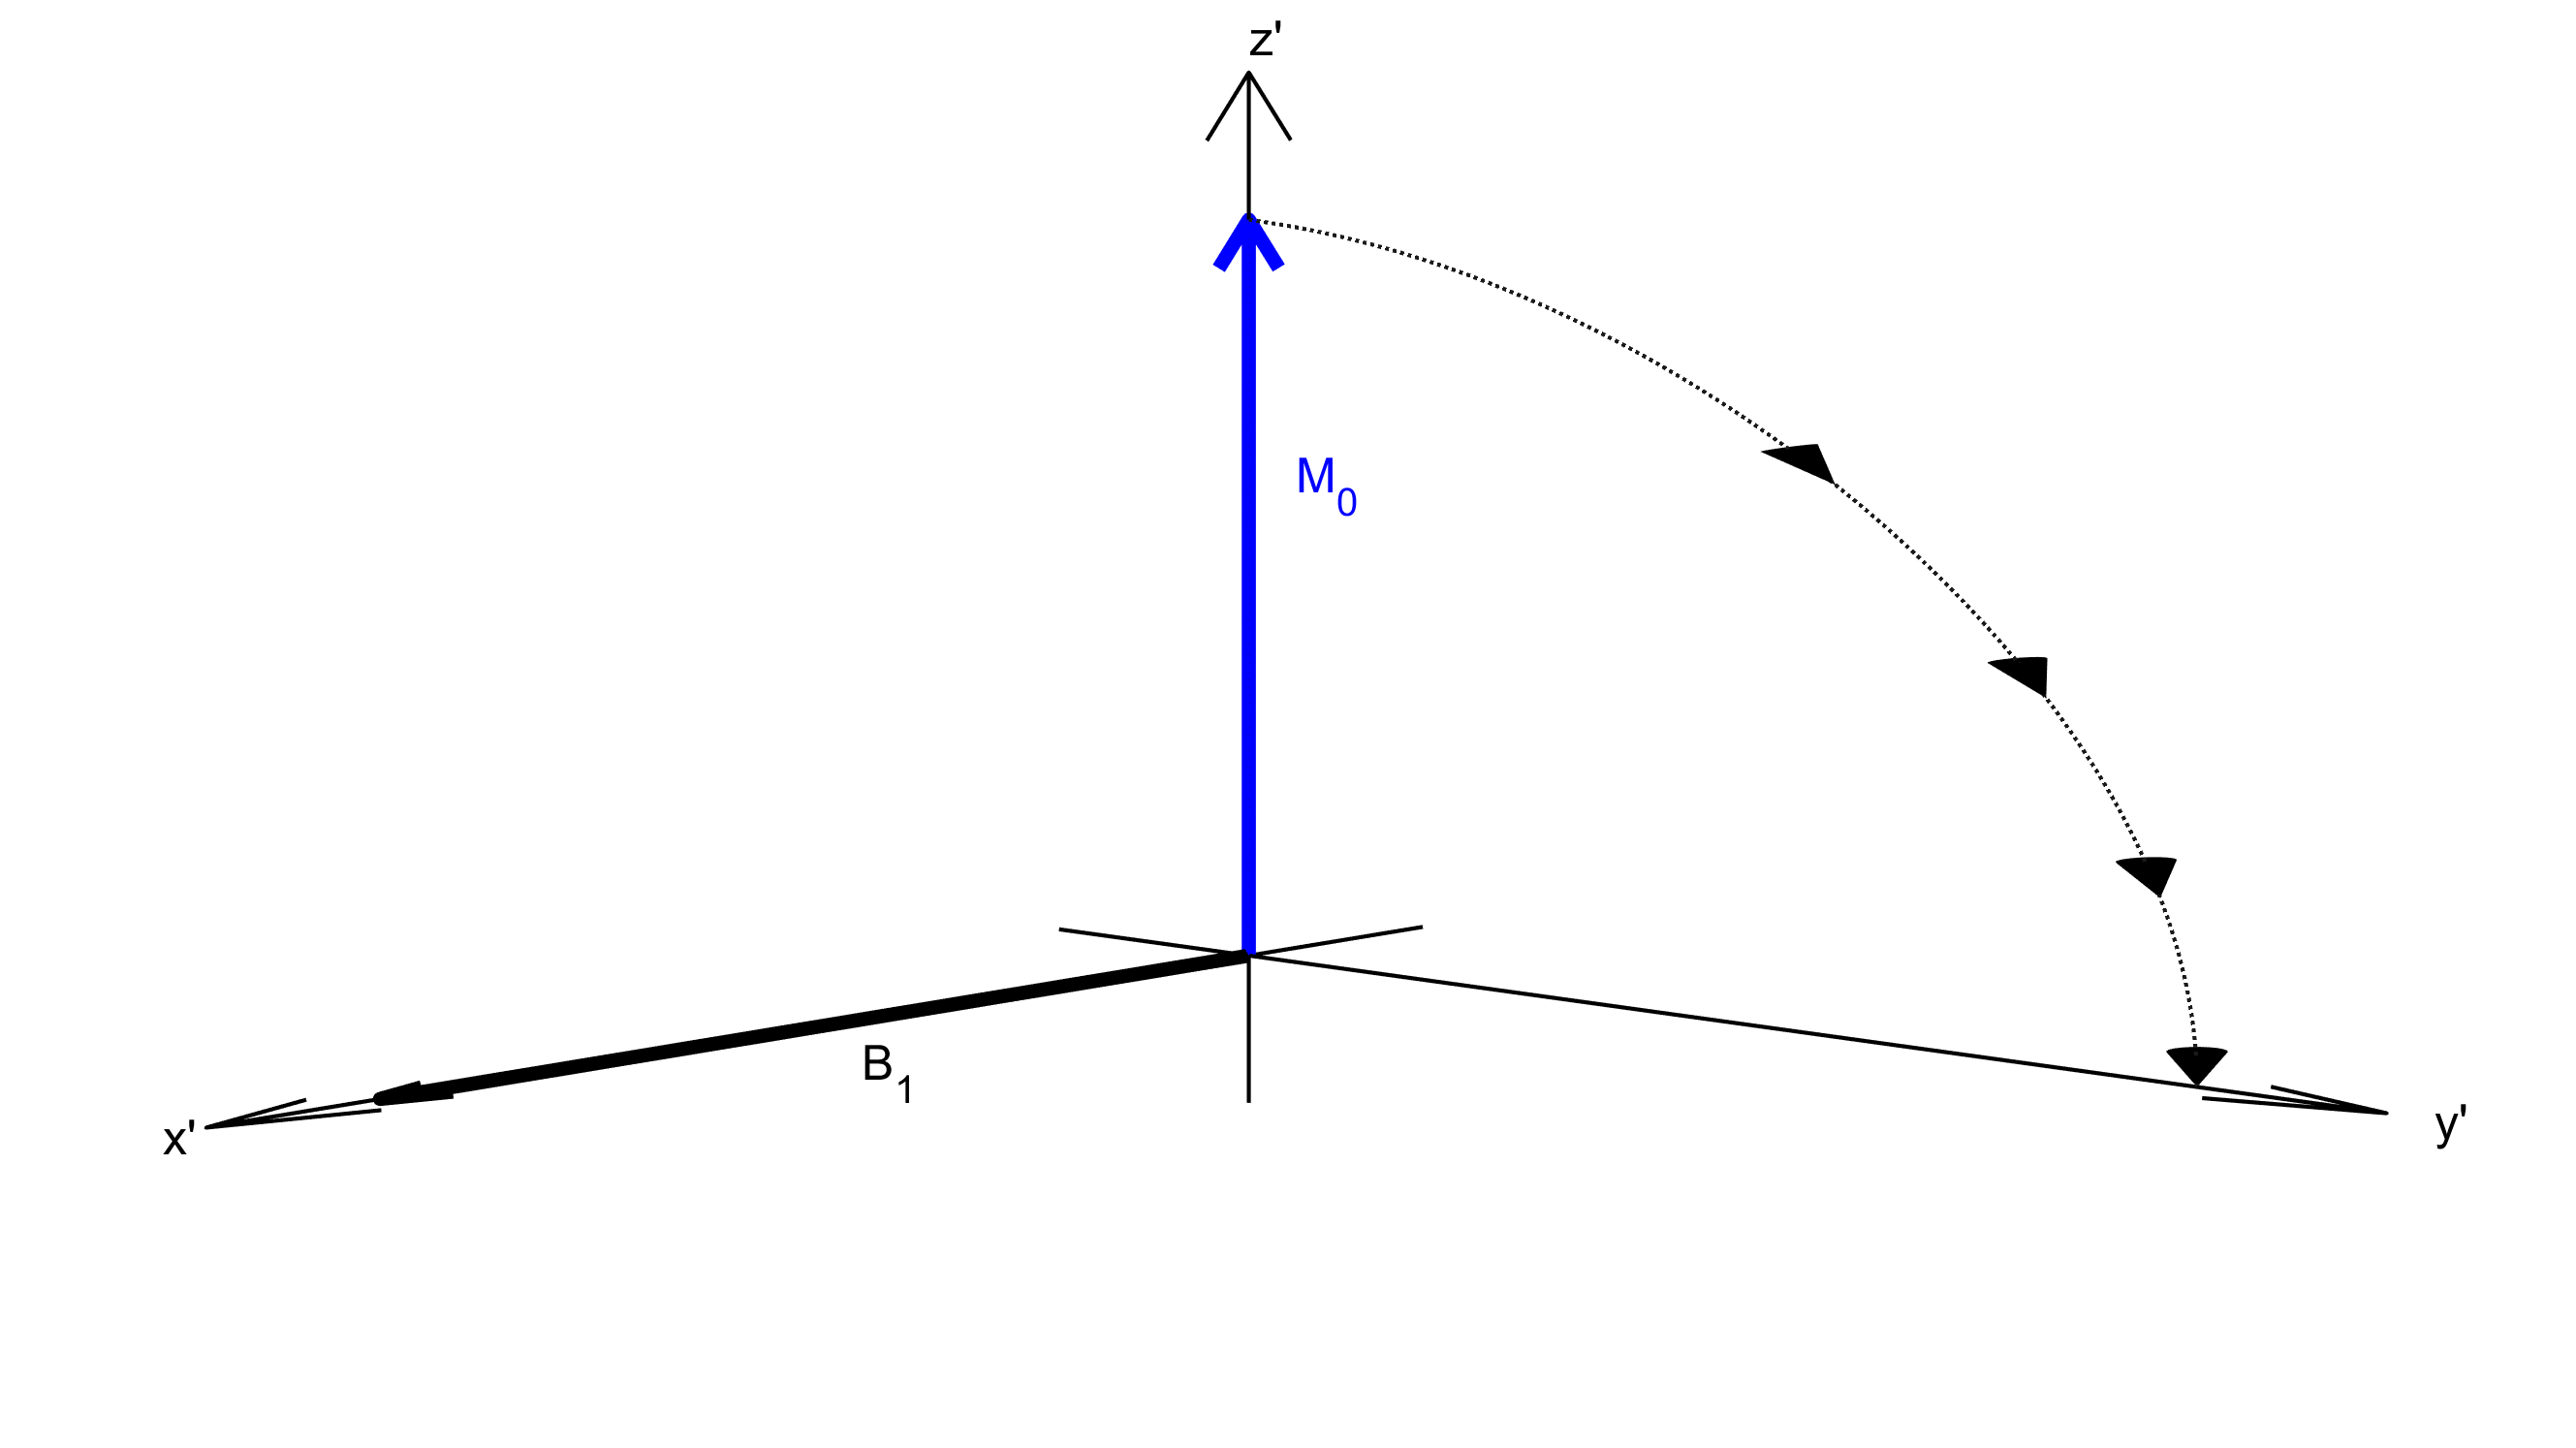
\includegraphics[width=\textwidth]{figures/background/nutation_onres.eps}
	\caption[Motion of a spin in the presence of a $B_1$ \ac{RF} field in the rotating frame]{Motion of a spin in the presence of a $B_1$ RF field in the rotating frame. This is identical to the nutation in \Cref{fig:nutation}, however viewing from the rotating frame simplifies the motion. }
	\label{fig:onres}
\end{figure}

This situation is known as resonance - the frequency of the \ac{RF} pulse matches the Larmor frequency, perfectly tipping the magnetisation away from the $z'$ axis and into the transverse plane. 

In the off-resonance case, an additional component of magnetic field with magnitude $\Omega/\gamma$ is produced in the $z$-direction.
This results in an effective magnetic field, $\mathbf{B}_e$, with a magnitude \cite{DeGraaf2007}
\begin{equation}
	B_e = |B_e| = \sqrt{B_1^2 + \left(\frac{\Omega}{\gamma}\right)^2}\,.
	\label{eq:Beff}
\end{equation}

%\todo[inline]{Do I need this off-resonance stuff? It's more geared towards introducing chemical shift for MRS. Perhaps just focus on signal generation?}
The effective field is illustrated in \Cref{fig:B_e} with the additional component of $\Omega/\gamma$ resulting in an effective field that is no longer aligned with $x'$.
\begin{figure}
	\centering
	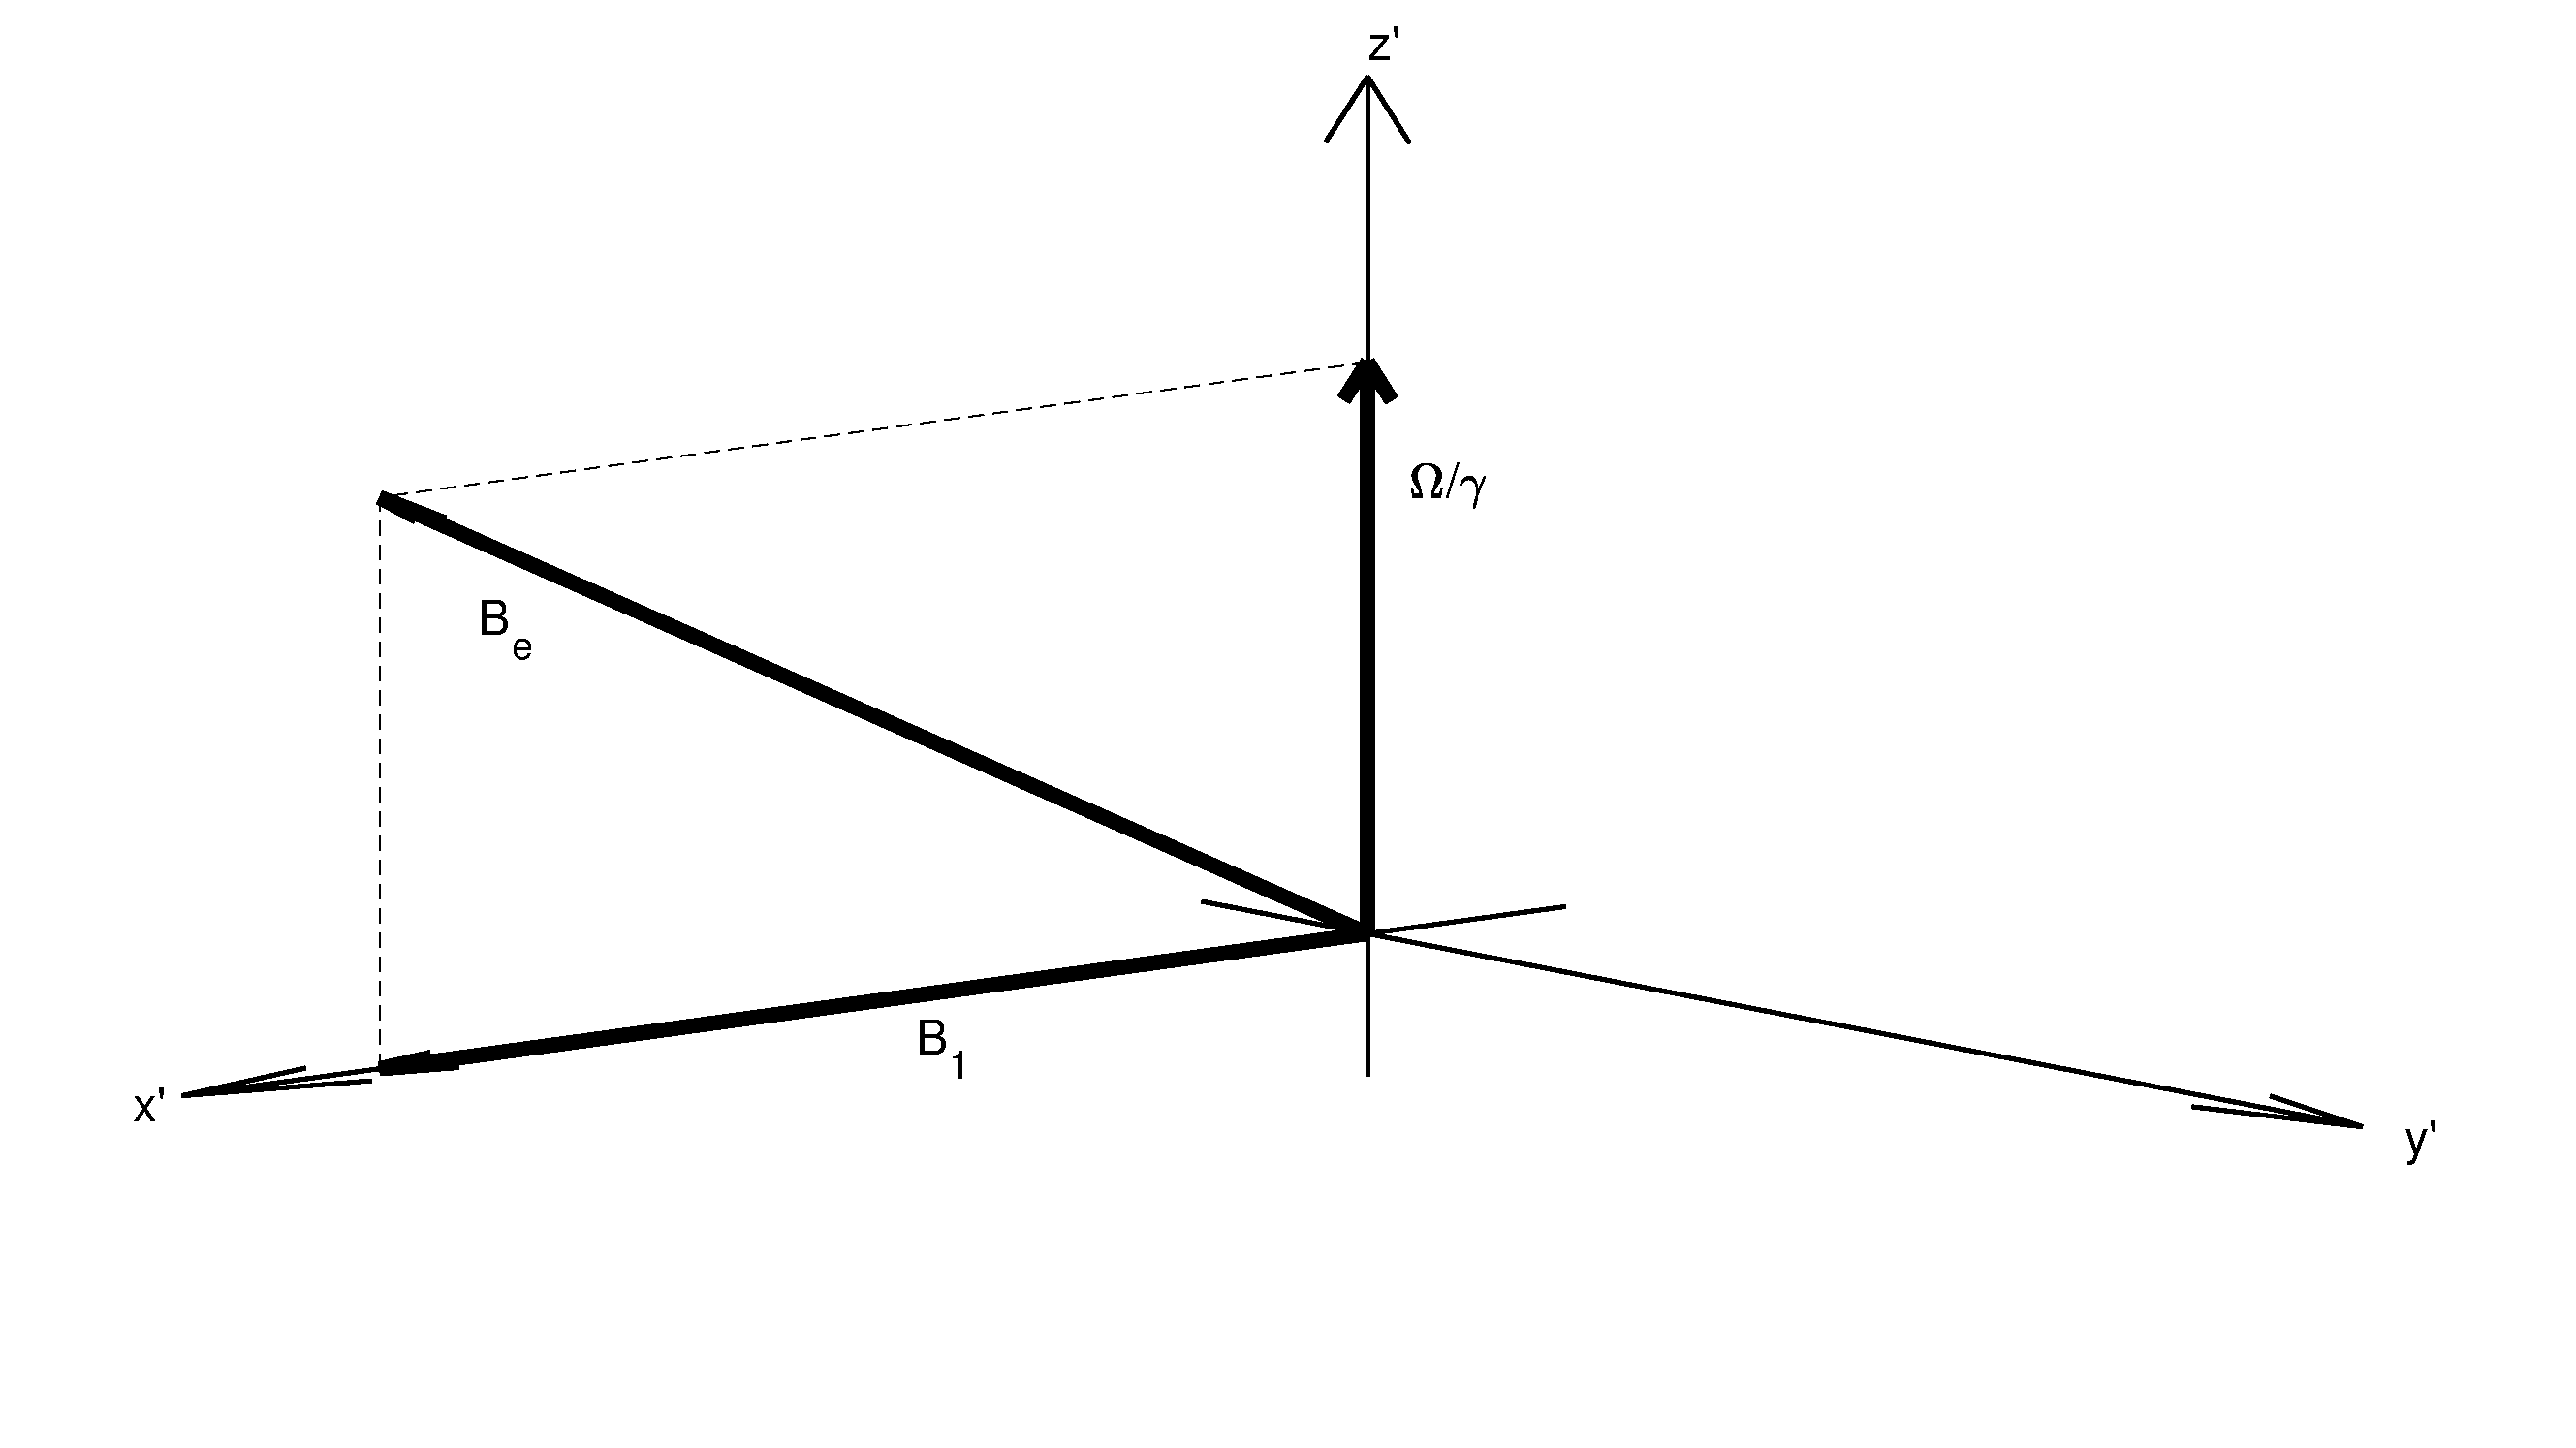
\includegraphics[width=\textwidth]{figures/background/B_e.eps}
	\caption[The effective field, $B_e$, produced due to an off-resonance frequency $\Omega$.] {The effective field, $B_e$, produced due to an off-resonance frequency $\Omega$. The off-resonance effects produce an additional component of magnetic field along the $z'$ axis.}
	\label{fig:B_e}	
\end{figure}
Off-resonance effects can produce unwanted results meaning the spin does not get flipped as much as expected under an \ac{RF} pulse which can result in signal losses. 
 

\subsection{Detecting the MR Signal}
The detection and processing of \ac{NMR} signals is a deep topic which could be the subject of its own book, however some very basic details of how a signal is formed are useful to go on from here.
 
The reason for flipping the magnetisation into the transverse plane using $\mathbf{B}_1$ fields is to make the magnetisation detectable. 
Transverse magnetisation precesses about $\mathbf{B}_0$ at the Larmor frequency, sweeping its magnetic field around $\mathbf{B}_0$. 
A coil of wire placed near this precessing field will feel an electromotive force induced in it according to Faraday's Law of Induction\cite{Haacke1999}.

Following a pulse that flips the magnetisation from $\mathbf{M}_0$ aligned with $z$ through an angle $\beta$ towards $x'$, the $x'$-component of the magnetisation will be $M_0\sin\beta$ and (ignoring relaxation) will then precess at the offset frequency, $\Omega$, in the rotating frame. This will give the components of the magnetisation in the transverse plane over time as 
\begin{equation}
M_x = M_0\sin(\beta)\cos(\Omega t) \qquad M_y = M_0\sin(\beta)\sin(\Omega t)\,.\label{eq:MxMy}
\end{equation}

The signal induced into the receiver coils is proportional to $M_x$ and $M_y$ and so the signal will also have an oscillating form similar to \Cref{eq:MxMy}.
From the $\sin\beta$ term, it is clear that the maximum signal will arise when $\beta = 90$\degree, meaning all the magnetisation is flipped into the transverse plane. 
Additionally, in a realistic experiment, there will be $\mathrm{T_2^*}$ relaxation so including this, the general form of the signal following a 90\degree\ pulse will be\cite{DeGraaf2007} 
\begin{equation}
S_x = S_0\cos(\Omega t)\exp\left(-t/\mathrm{T}_2^*\right) \qquad S_y = S_0\sin(\Omega t)\exp\left(-t/\mathrm{T}_2^*\right)\,.
\end{equation}

Generally \ac{NMR} systems use something known as quadrature detection, meaning that both the $x'$ and $y'$ components of the magnetisation are measured simultaneously\cite{Levitt2008}, giving the signal as a function of time as 
\begin{align}
	S(t) &= S_x + iS_y\,,\nonumber\\
		 &= S_0\exp((i\Omega - 1/\mathrm{T}_2^*)t)\,.\label{eq:fid}
\end{align}  

\begin{figure}
  \centering
  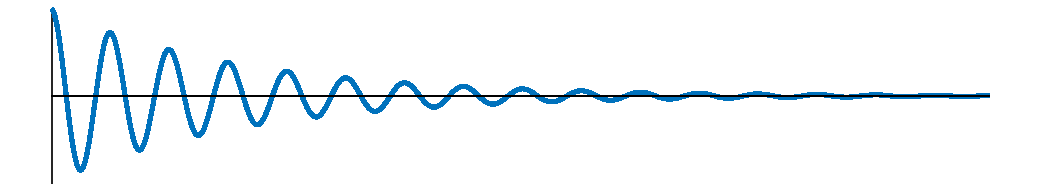
\includegraphics[width=\textwidth]{figures/background/FID_copy.png}
  \caption[The \acl{FID} described by \Cref{eq:fid}]{The \acl{FID} described by \Cref{eq:fid}. Here, just the real channel is plotted.}
  \label{fig:fid}
\end{figure}

This time-domain signal is known as a \ac{FID} and has a typical form shown in \Cref{fig:fid}. 
If we neglect off-resonance effects, then the \ac{FID} in the rotating frame will be a simple exponential decay.
\begin{equation}
  S(t) = S_0\exp(-t/\mathrm{T}_2^*)
  \label{eq:fid_rotframe}
\end{equation}

The \ac{FID} is not commonly used for \ac{dMRI} for a few reasons. Firstly, magnetic field gradients need to be introduced to make the signal sensitive to diffusion. Additionally, the $\mathbf{T}_2^*$ decay is often very rapid, so sequences known as spin echo sequences are used to remove the $\mathbf{T}_2'$ relaxation. 

\begin{comment}
The \ac{FID} holds all of the relevant information about the spin system needed for \ac{NMR}, however it is seldom used on its own since the information is difficult to interpret in this form.
\ac{NMR} spectroscopy uses a mathematical procedure known as the Fourier transform which is used as a transformation between the time and frequency domains. 
\begin{figure}
	\centering
	\begin{subfigure}{\textwidth}
		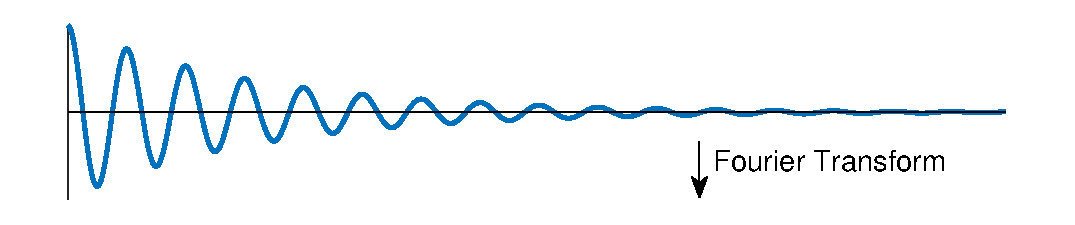
\includegraphics[width=\textwidth]{figures/background/FID.eps}
	\end{subfigure}

	\begin{subfigure}{\textwidth}
		
\includegraphics[width=\textwidth]{figures/background/fftFID.eps}
	\end{subfigure}
	\caption{An example of the Fourier transform. The time domain signal (top) is transformed into a frequency domain (bottom) by the Fourier transform. }
	\label{fig:fft}

      \end{figure}
      
Many books cover the Fourier transform in great detail \cite{Keeler2010, Haacke1999}, however for this report, it is sufficient to simply know its results.
The Fourier transform will take an \ac{FID} signal of the form in \Cref{eq:fid} and produce a frequency domain signal that has a mathematical form known as a Lorentzian, given by 
\begin{equation}
	S_0\exp((i\Omega - R_2)t) \quad\overset{\mathrm{FT}}{\rightarrow}\quad \frac{S_0R_2}{R_2^2 + (\omega - \Omega)^2} + i\frac{S_0(\omega - \Omega)}{R_2^2 + (\omega - \Omega)^2}\,,
\end{equation}    
where $\omega$ is the frequency domain of the spectrum. 
The real part of this term is known as the absorption mode and the imaginary part is known as the dispersion mode.
The absorption mode Lorentzian is shown in the bottom plot in \Cref{fig:fft}. 
Peaks like this form the basis of all spectra used in \ac{NMR} spectroscopy. 
\end{comment}



\subsection{Spin Echoes}
\label{sec:spin_echoes}
\begin{figure}
	\centering
	\begin{subfigure}{0.9\textwidth}
		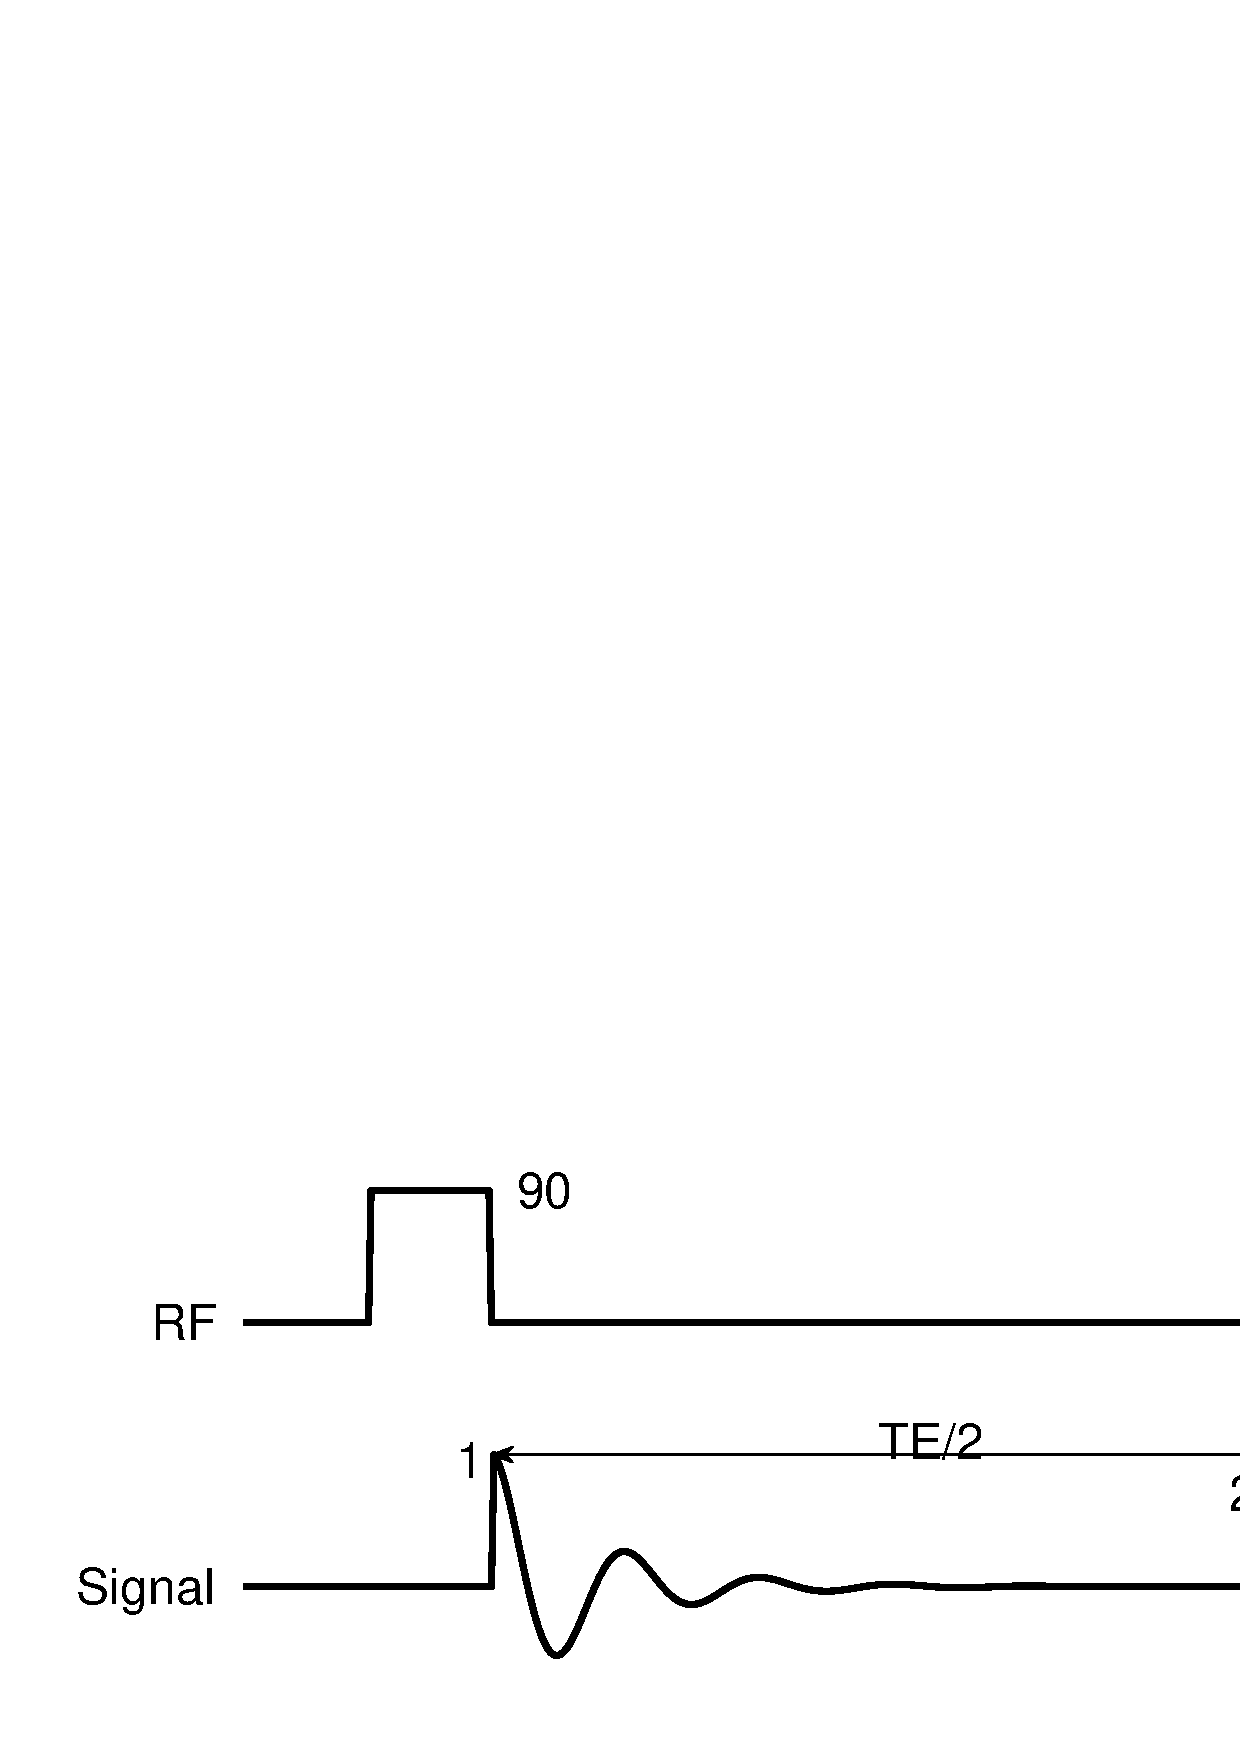
\includegraphics[width = \textwidth]{figures/background/spinecho.png}
		\caption{}
		\label{fig:spinechosequence}
	\end{subfigure}
	
	\begin{subfigure}{0.9\textwidth}
		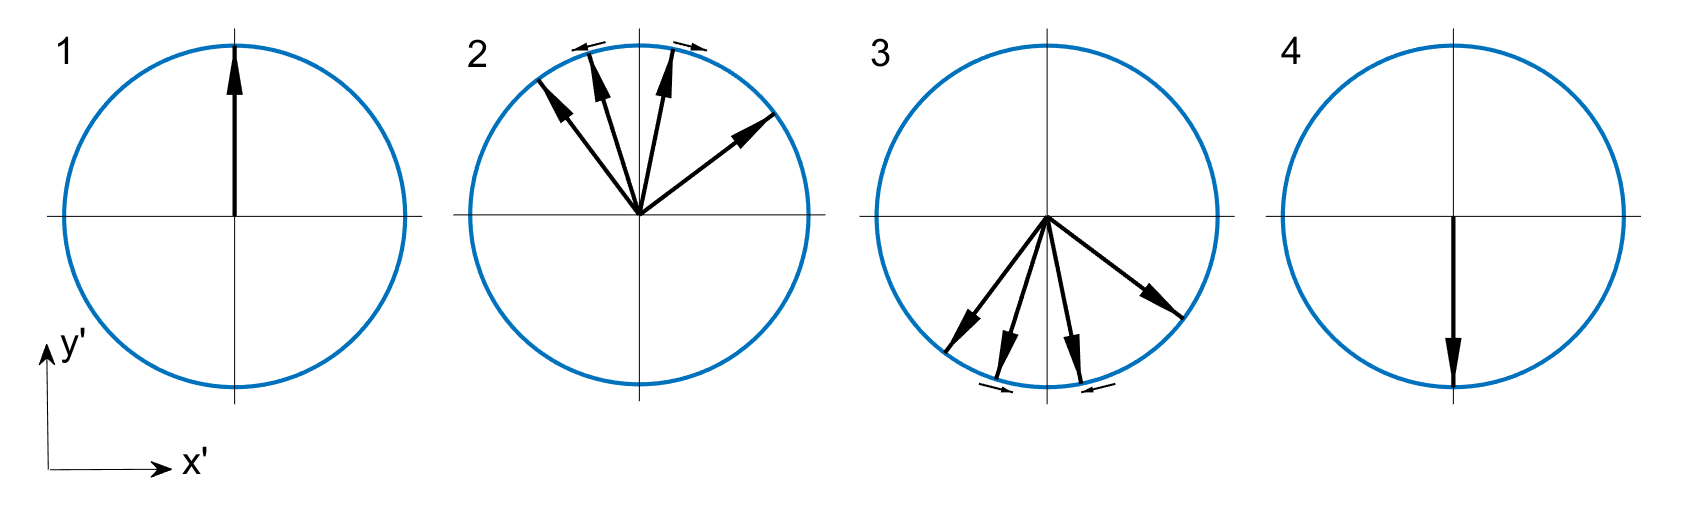
\includegraphics[width = \textwidth]{figures/background/spinecho_evolution.eps}
		\caption{}
		\label{fig:spinecho_evolution}
	\end{subfigure}

	\caption[The spin echo sequence and the evolution of spin under a spin echo sequence.]{a) Spin echo sequence and (b) an indication of the evolution of spins under a spin echo sequence. This shows how the 180\degree\ refocusing pulse acts to refocus the spins after a time $\mathrm{TE}$.}
	\label{fig:spinecho}
\end{figure}
It is possible to undo the effects of $\mathrm{T}_2'$ by designing a pulse sequence to `refocus' the spins, forming what is known as a spin echo.
%Spin echo sequences also enable localisation by combining \ac{RF} pulses with magnetic field gradients.
The first spin echo sequence was introduced by Edwin Hahn in 1950 \cite{Hahn1950}. The simplest sequence to form a spin echo consists of a 90\degree\ pulse to excite the spins followed by a 180\degree\ pulse after a delay. 
This sequence is shown in the diagram in \Cref{fig:spinecho} along with how the signal varies during the pulse sequence.
 
\Cref{fig:spinecho_evolution} represents how the magnetisation evolves through the pulse sequence with the four diagrams corresponding to the points marked in \Cref{fig:spinechosequence}. 
At point 1, immediately following the 90\degree\ pulse, all the magnetisation has been flipped into the transverse plane and is in phase - meaning all the magnetic moments of the spins point in the same direction in the x-y plane. 

The field inhomogeneities cause the different spins to feel slightly different magnetic fields and so precess at slightly different frequencies. 
This causes the spins to lose phase-coherence as indicated at point 2, and so the signal decays with $\mathrm{T}_2^*$.  

At point 3, following the 180\degree\ pulse, the spins remain out of phase with one another, but the 180\degree\ pulse has flipped their orientations across the $x'$-axis. 
The magnetic field the spins feel is still the same, so despite their flip in orientation, they still precess in the same direction. 
This means that the evolution that caused the spins to dephase begins to rewind and bring the spins back into phase coherence. 
After a time equal to the time between the 90\degree\ and 180\degree\ pulses, at point 4, the spins will be brought completely back in phase - or, refocused - and the spin echo is formed. 

The signal at point 4 will still be lower in magnitude than that at point 1 since the $\mathrm{T}_2$ relaxation will still occur as it is an inherent property of the matter. 
The spin echo does, however, refocus the $\mathbf{B}_0$ inhomogeneities. 
The time between the 90\degree\ pulse and the formation of the echo is known as the \ac{TE}. 

The spin echo sequence shown in \Cref{fig:spinecho} forms the basis of the standard \ac{PGSE} diffusion MRI sequence which is introduced in the following section, along with a description of the physics behind diffusion MRI. 

\section{Diffusion MRI}
\label{sec:diffusion_physics}
Diffusion MRI (dMRI) sensitises the \ac{MRI} signal to the motion of water molecules due to diffusion. The following section describes the physics behind diffusion and how the diffusion impacts the \ac{MRI} signal.

% Diffusion MRI simulations attempt to synthesise dMRI signals through models of our understanding of the underlying diffusion processes.
% These simulations broadly fall into two categories: solutions of the diffusion equation and Monte-Carlo simulations of the diffusion dynamics.

% The diffusion equation relates the rate of change of concentration to the spatial variation in concentration according to
% \begin{equation}
%   \frac{\partial c(\vec{r}, t)}{\partial t} = D\nabla^2 c(\vec{r}, t)\,.
% \end{equation}
%Diffusion \ac{MRI} simulations are ultimately trying to synthesise the \ac{dMRI} signal through models of our understanding of the underlying diffusion processes.
%This section briefly covers the physics that gives rise to the \ac{dMRI} signal. 

The diffusion process is driven by the Brownian motion of particles in fluids.
The thermal kinetic energy of particles causes them to move around rapidly, however particles frequently collide with each other (for instance, molecules in water at room temperature experience around 60 billion collisions per second \cite{Denny1993}) creating a very tortuous, random path.

Diffusion \ac{MRI} sensitises the MR signal to this motion by exploiting the dephasing of spins as a result of magnetic field gradients.


The magnetic field will generally have a uniform component from the main $B_0$ field, and spatially and/or time varying components due to deliberate magnetic field gradients or typically unwanted effects such as magnetic susceptibility inhomogeneities and concomitant fields \cite{Haacke1999}. In general, $B(\mathbf{r}, t)$, the magnitude of the magnitude of the magnetic field at a position $\mathbf{r}$ at time $t$ is given by
\begin{equation}
  B(\mathbf{r}, t) = |\mathbf{B}| = |B_0\mathbf{\hat{z}} + \mathbf{\Delta B}(\mathbf{r}, t)|\,,
  \label{eq:mod_B}
\end{equation}
where $\mathbf{\Delta B}(\mathbf{r}, t)$ accounts for all of the variation in the magnetic field away from $B_0$. Note that $\mathbf{\Delta B}(\mathbf{r}, t)$ is a vector quantity which may have components in the $\mathbf{\hat{x}}$ and $\mathbf{\hat{y}}$ directions. 

An idealised expression for $\mathbf{\Delta B}(\mathbf{r}, t)$ often applied to \ac{MRI} assumes that all of the change in the magnetic field is due to an applied magnetic field gradient, $\mathbf{g}(\mathbf{r}, t)$, which only has a significant $\mathbf{\hat{z}}$ component. This means that \Cref{eq:mod_B} can be written as
\begin{align}
  B(\mathbf{r}, t) &= \left|B_0\mathbf{\hat{z}} + \left(\mathbf{g}(\mathbf{r}, t)\cdot\mathbf{r}\right) \mathbf{\hat{z}}\right|\,,\nonumber \\
                      &= B_0 + \mathbf{g}(\mathbf{r}, t)\cdot\mathbf{r}\,.
                        \label{eq:mod_B_ideal}
\end{align}

Magnetic field gradients introduce a deliberate variation in the magnetic field which, according to \Cref{eq:LarmorFreq}, causes the Larmor frequency to vary spatially as well temporally.

Since the Larmor frequency varies spatially, spins in different locations will precess at different frequencies and accrue a phase shift relative to spins in different locations. 
The incremental phase, $d\phi$, accrued for a single spin, $i$, in an infinitesimal time, $dt$, % assuming a gradient in the $z$ direction
is given by
\begin{equation}
  % \phi(t, \mathbf{g}(\mathbf{r}(t), t)) = \gamma B_0 t + \gamma \int_0^t \mathbf{g}(\mathbf{r}(t'), t')\cdot\mathbf{r}(t')dt'\,,
  % \label{eq:phase_singlespin}
  d\phi_i = \gamma B(\mathbf{R}_i(t), t) dt\,,
  \label{eq:dphi}
\end{equation}
% where $\gamma$ is the gyromagnetic ratio, $B_0$ is the main field strength, $\mathbf{r}(t')$ is the position of the particle and $\mathbf{g}(\mathbf{r}(t'), t')$ is the (potentially spatially varying and time-dependent) magnetic field gradient.
where $\gamma$ is the gyromagnetic ratio and  $\mathbf{R}_i(t)$ is the position of the particle at time $t$. %and $B(\mathbf{r}(t), t)$ is the magnitude of the magnetic field at position $\mathbf{r}(t)$ and time $t$.

Putting \Cref{eq:mod_B_ideal} into \Cref{eq:dphi} and integrating over the time of the diffusion experiment will give the total phase accrued for a single spin:
\begin{equation}
  % \phi(t, \mathbf{g}(\mathbf{R}_i(t), t)) = \gamma B_0 t + \gamma \int_0^t \mathbf{g}(\mathbf{R}_i(t'), t')\cdot\mathbf{R}_i(t')dt'\,,
  \phi(\mathbf{R}_i(t)) = \gamma B_0t + \gamma\int_0^t\mathbf{g}(\mathbf{R}_i(t'), t')\cdot\mathbf{R}_i(t')dt'\,,
  \label{eq:phase_singlespin}
\end{equation}


The first term in this equation is the phase accrued due to the main magnetic field which will be the same for all spins in the system.
The second term is the phased accrued due to the gradient, which will be dependent on the motion of each individual spin.
The dot product here indicates that only displacement projected onto the gradient direction affects the phase, allowing the gradient direction to be used to probe the diffusion in different directions.

\begin{figure}
  \centering
  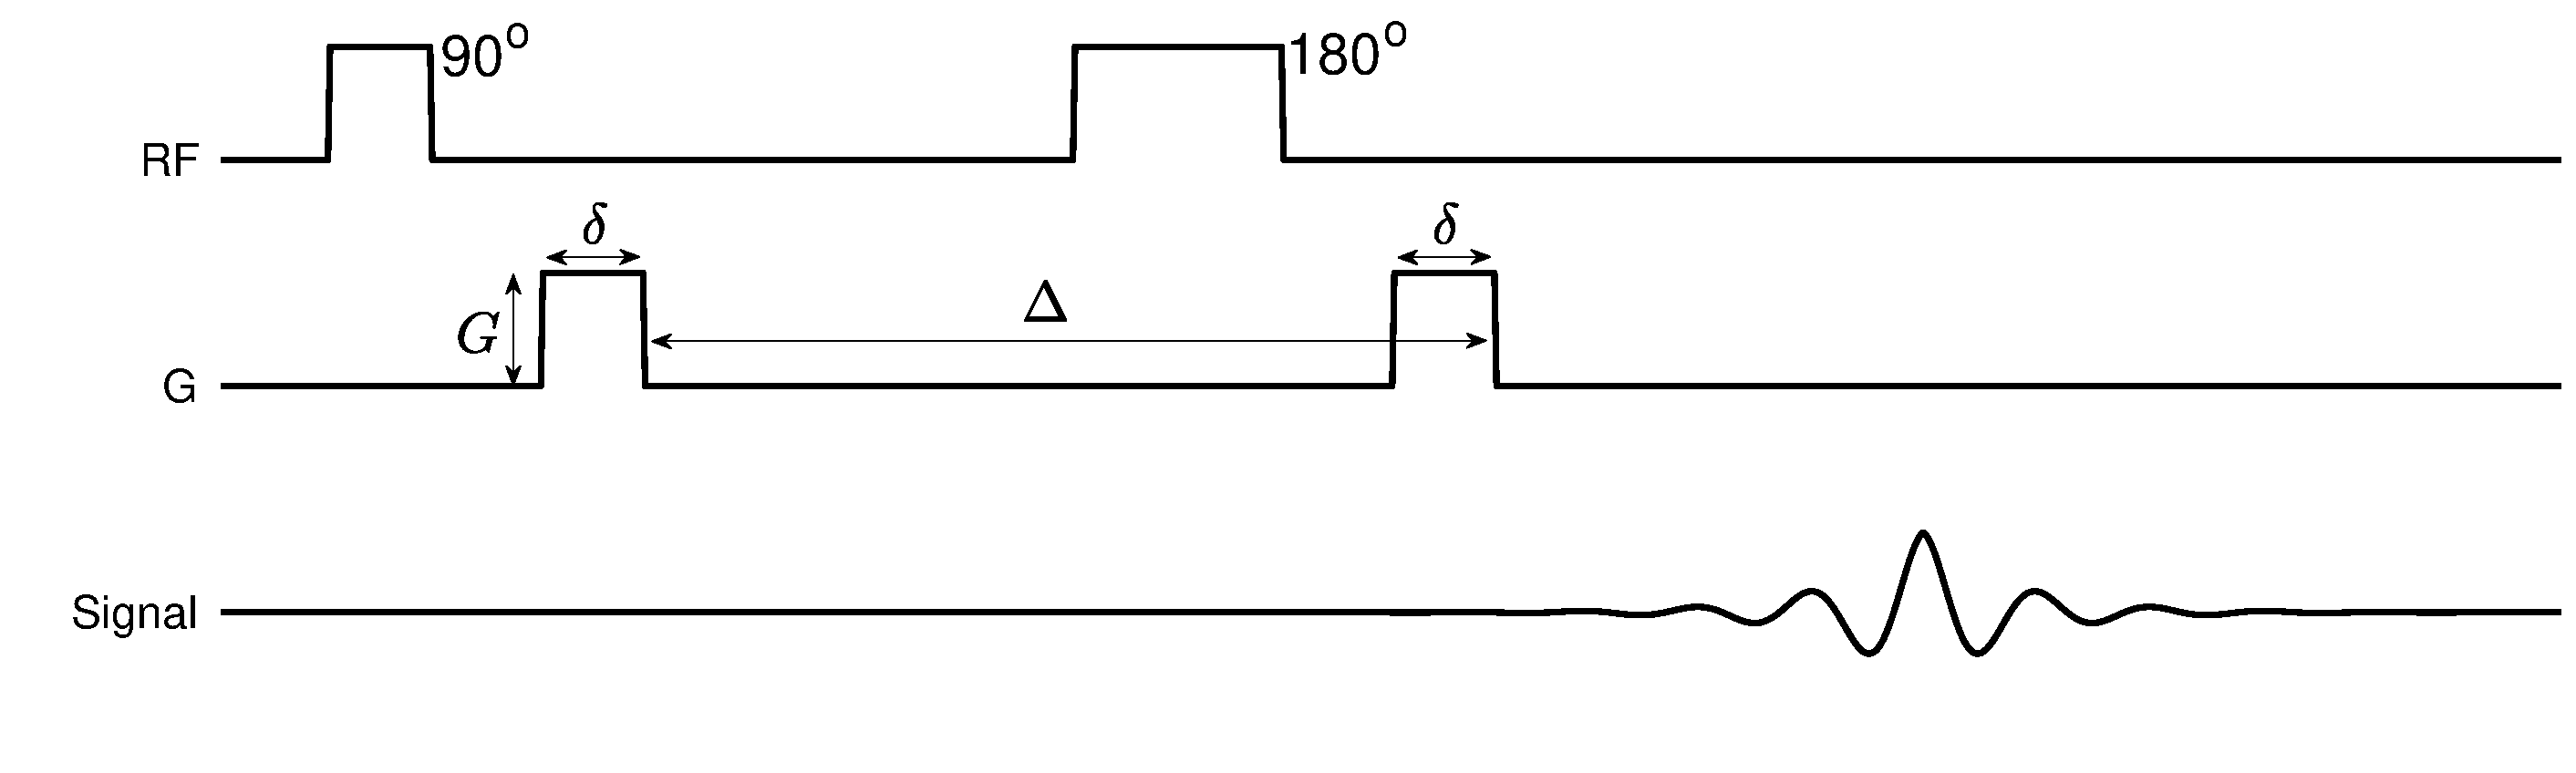
\includegraphics[width=0.9\textwidth]{figures/background/PGSE_diagram.eps}
  \caption{The standard \acl{PGSE} sequence used in \ac{dMRI}.}
  \label{fig:PGSE_diagram}
\end{figure}

The first diffusion MR sequence, introduced by Stejskal and Tanner in 1965\cite{Stejskal1965}, is the \acf{PGSE} sequence, shown in \Cref{fig:PGSE_diagram}.
The PGSE sequence consists of a standard spin echo sequence with a pair of gradient pulses added either side of the refocussing pulse.
In the ideal case, each pulse is rectangular with a gradient strength, $G$, and duration, $\delta$ and they are separated by a time, $\Delta$.  

The effect of this pulse sequence can be simplified by considering the case when $\delta \ll \Delta$. This is known as the \ac{SGP} approximation and means that the motion of spins during the pulses can be ignored. 

Under the \ac{SGP} approximation, the phase accrued by a spin at a position $\mathbf{R}_0$ during a pulse at a time $t_0$ will be
\begin{equation}
  \phi(\mathbf{R}_0) = \gamma B_0\delta +  \gamma \delta \mathbf{g(R_0)}\cdot\mathbf{R_0}\,.
  \label{eq:phi_single_SGP}
\end{equation}
Here, $\mathbf{R}_0$ refers to the spin position at time $t=t_0$ and is not time-dependent, because under the SGP approximation the motion of spins during the pulse is assumed to be negligible. 

The 180\degree\ pulse in the \ac{PGSE} sequence is crucial, since it flips the orientation of the spins' magnetic moments as in the spin echo sequence in \Cref{fig:spinecho}.
Not only does this refocus $\mathrm{T}_2^*$ effects as outlined in \Cref{sec:spin_echoes}, but similarly, it means that the phase accrued due to the first gradient pulse now has a negative sign relative to the phase that will be accrued due to the second pulse. %due to the second gradient pulse has opposite sign to the phase accrued due to the first pulse. 

A spin which is at a position $\mathbf{R}_0$ during the first pulse and then diffuses to a position $\mathbf{R}_1$ during the second pulse will therefore have a relative phase shift of 
\begin{equation}
  \Delta\phi(\mathbf{R}_1 - \mathbf{R}_0) = \gamma\delta\mathbf{g} \cdot \left(\mathbf{R}_1 - \mathbf{R}_0\right)\,.
  \label{eq:delta_phi}
\end{equation}

The $B_0$ term from \Cref{eq:phi_single_SGP} is the same for both gradient pulses, meaning that during the subtraction in \Cref{eq:delta_phi} it cancels and the only relative phase shift comes from the diffusive motion.

The total MR signal comes from an ensemble of spins, each with their own random Brownian motion and thus, from \Cref{eq:delta_phi}, their own relative phase shift.
To get to the total MR signal, we need to consider the probability that a particle starts at position $\mathbf{R}_0$ (i.e. the initial spin density, $\rho(\mathbf{R}_0)$, which can generally be considered uniform within a voxel \cite{Price1997}) and the probability that a particle which starts at $\mathbf{R}_0$ moves to $\mathbf{R}_1$ during the time $\Delta$, $P(\mathbf{R}_0, \mathbf{R}_1, \Delta)$.
Putting these together, gives an expression for the total MR signal\cite{Price1997,Stejskal1965}:
\begin{equation}
  S(\mathbf{g}, \Delta) = S(\mathbf{0}, \Delta)\int\int \rho(\mathbf{R}_0)P(\mathbf{R}_0, \mathbf{R}_1, \Delta) e^{i\gamma\delta\mathbf{g} \cdot (\mathbf{R}_1 - \mathbf{R}_0)}  d\mathbf{R}_0d\mathbf{R}_1\,.
  \label{eq:total_signal_sgp}
\end{equation}

This quantity, $P(\mathbf{R}_0, \mathbf{R}_1, \Delta)$, is known as the diffusion propagator and is of great interest for diffusion MRI because $P(\mathbf{R}_0, \mathbf{R}_1, \Delta)$ encodes the information about the environment in which the spins are diffusing. 
For diffusion in an isotropic, homogeneous medium, the diffusion propagator is a Gaussian distribution \cite{Price1997}:
\begin{equation}
  P(\mathbf{R}_0, \mathbf{R}_1, t) = \left(4\pi Dt\right)^{-\sfrac{3}{2}}\exp\left(-\frac{(\mathbf{R}_1 - \mathbf{R}_0)^2}{4Dt}\right)\,.
  \label{eq:propagator_diffusion}
\end{equation}

In the case of Gaussian diffusion, \Cref{eq:total_signal_sgp} can be solved analytically and will give an MR signal attenuation (that is, $S(t)/S(0)$) which is also Gaussian\cite{Stejskal1965,Price1997}
\begin{equation}
  E(g, \Delta) = \exp(-\gamma^2g^2\delta^2D\Delta)\,.
  \label{eq:sgp_signal_gaussian}
\end{equation}

The general form of this expression, accounting for finite duration gradient pulses, can also be analytically derived to give the Stejskal-Tanner equation \cite{Stejskal1965,Kuchel2012}
\begin{align}
  \ln(E) &= -\gamma^2g^2\delta^2D(\Delta - \delta/3)\,,\label{eq:stejskal_tanner}\\
  &= -bD\,,
\end{align}
where $b = \gamma^2g^2\delta^2(\Delta - \delta/3)$ is the so-called $b$-value which describes the strength of the diffusion encoding. 

We can formulate a more general form of  \Cref{eq:total_signal_sgp} without requiring any assumptions on the gradients (such as the \ac{SGP} approximation used above) as \cite{Price1997,Hall2009}
\begin{equation}
  S(\mathbf{g}, t) = S(\mathbf{0}, t) \int_{-\infty}^{\infty} P(\phi, t) e^{i\phi} d\phi\,,
  \label{eq:sig_phi_complex}
\end{equation}
where the phase, $\phi$ will be given by \Cref{eq:phase_singlespin} and $P(\phi, t)$ is the probability density function of the phase distribution after a time $t$.

In the case of restricted diffusion (i.e.\ diffusion in an inhomogeneous or anisotropic environment) the form of the diffusion propagator becomes more complex and closed form solutions of \Cref{eq:total_signal_sgp,eq:sig_phi_complex} are only possible for certain simple geometries and assumptions.

Analytical solutions can be found for some simple restricting geometries such as spheres, cylinders and parallel plates \cite{Neuman1974, Balinov1993,Callaghan1995}.
For more complex environments, however, an analytical solution is intractable and we must rely on simulations to approximate the \acl{dMRI} signal.  

\begin{comment}
The total MR signal comes from an ensemble of spins, each with their own random Brownian motion and thus, from  \Cref{eq:phase_singlespin}, their own phase. This gives the total \ac{dMRI} signal, $S(t, \mathbf{g})$ as

where $S(t, \mathbf{0})$ is the signal with no gradients applied. $P(\phi, t)$ is the probability density function of the phase distribution after a time $t$.

From \Cref{eq:phase_singlespin}, we see that the individual phases, and thus the phase distribution, depend on the motion of the particles as well as the description of the diffusion sensitising gradient (in the case of standard pulsed gradient experiment that is the timing, strength, duration and orientation of the gradient) \cite{Price1997}.

This quantity, $P(\phi, t)$, is closely related to another property of great interest for diffusion MRI known as the diffusion propagator, $P(\mathbf{R}_0, \mathbf{R}_1, t)$. $P(\mathbf{R}_0, \mathbf{R}_1, t)$ is the probability that a particle initially at a position $\mathbf{R}_0$ moves to $\mathbf{R}_1$ in a time $t$.
For diffusion in an isotropic, homogeneous medium, the diffusion propagator is a Gaussian distribution \cite{Price1997}:
\begin{equation}
  P(\mathbf{R}_0, \mathbf{R}_1, t) = \left(4\pi Dt\right)^{-\sfrac{3}{2}}\exp\left(-\frac{(\mathbf{R}_1 - \mathbf{R}_0)^2}{4Dt}\right)\,.
  \label{eq:propagator_diffusion}
\end{equation}

\end{comment}

\subsection{The \acl{BT} Equations}
\label{sec:bg_bloch_torrey}
As well as describing the \ac{dMRI} signal by considering the microscopic diffusion of spins, a macroscopic formulation can be derived considering Fick's laws of diffusion. The combination of the Bloch equations (\Cref{eq:blochx,eq:blochy,eq:blochz}) with Fick's second law of diffusion leads to the \ac{BT} equations, proposed by H.\ C.\ Torrey in 1956\cite{Torrey1956,Callaghan1991,Price2009}:

\begin{equation}
  \frac{\partial\mathbf{M(r},t)}{\partial t} = \gamma \mathbf{M \times B(r}, t) - \frac{M_x\mathbf{\hat{x}} + M_y\mathbf{\hat{y}}}{\mathrm{T}_2} - \frac{(M_z - M_0)\mathbf{\hat{z}}}{\mathrm{T}_1} + \nabla \cdot \left(\mathbf{D} \nabla \mathbf{M}\right)\,.
  \label{eq:bloch_torrey}
\end{equation}

This version of the \ac{BT} equation is sometimes referred to as the standard \ac{BT} equation. An additional term can be added to account for the evolution of the magnetisation due to a flow, described by a velocity field $\mathbf{v}$ to get the generalised \ac{BT} equation \cite{Jeener2002,Beltrachini2016}. However, this flow term is often dropped, assuming no net flow, in the application to \ac{dMRI}, leaving \Cref{eq:bloch_torrey}. 
$\mathbf{D}$ is the diffusion tensor, a generalisation of the diffusion coefficient, $D$, to allow for anisotropic diffusion. In short, this means that diffusion happens at a different rate in different directions.
It is the $\mathbf{D}$ term in \Cref{eq:bloch_torrey} which encodes the evolution of the magnetisation when there is diffusion.

In general, the \ac{BT} equations cannot be solved analytically, apart from in some simple cases such as isotropic free diffusion.
For instance, the solution to the \ac{BT} equations in isotropic free diffusion can be shown to give the expected Stejskal-Tanner equation, \Cref{eq:stejskal_tanner} \cite{Price1997}.

For complex geometries, as with the case above, we must rely on computational methods to come to a solution for the \ac{BT} equations. 



\section{Diffusion Simulation}
\label{sec:diffusion_simulation}
Diffusion simulations attempt to evaluate \Cref{eq:sig_phi_complex} or \Cref{eq:bloch_torrey} computationally. Simulation approaches broadly fall into two categories: numerical solutions of the \ac{BT} equation and \ac{MC} simulations of the diffusion dynamics. This section introduces these techniques, highlighting the some of the similarities and differences between them. 


At a high level, all diffusion simulations have three common components: the substrate, the diffusion dynamics and the measurement.
The substrate describes the environment in which the diffusion is taking place. A common example of this is parallel cylinders representing axons in white matter.
The diffusion dynamics describe our understanding of the processes underlying the diffusive motion of molecules and the measurement describes how this diffusive motion results in a synthetic \ac{dMRI} signal.
\subsection{Numerical Solutions}
\label{sec:numerical_solutions}
Numerical solution approaches generally attempt to solve the \acl{BT} equation \cite{Torrey1956}.
These approaches combine both the dynamics and the measurement components of the diffusion simulation by solving for the magnetisation in  \Cref{eq:bloch_torrey}.
The third component, the substrate, defines boundary conditions required for the solution of the equation. 

There are two typical methods for solving the \ac{PDE} in \Cref{eq:bloch_torrey}, \acp{FDM} and \acp{FEM}.
Finite difference methods evaluate the \ac{PDE} using a local Taylor expansion at discrete points which are generally uniformly separated in each spatial as well as the temporal dimension \cite{Grossmann2007}.
\acp{FDM} are an efficient method for solving \acp{PDE} when the problem can fit into a rectangular grid, however they are less effective when applied to complex geometries \cite{Hagslatt2003, Grossmann2007}.

Finite element methods subdivide the domain into small elements which are simple geometric shapes, though unlike the \acp{FDM}, they do not have to form a regular grid, but rather an arbitrary mesh.
In each element, the \ac{PDE} solution is approximated by simple functions such as a linear combination of polynomials.
The combination of all of these local approximations can be solved to give a numerical solution of the \ac{PDE} across the whole domain \cite{Logan2007}.
\acp{FEM} are generally more complex to formulate and implement than \acp{FDM}, however the added complexity can be worth the effort for more difficult problems in which \acp{FDM} may be ineffective \cite{Iserles2009}.

\subsection{Monte-Carlo Simulations}
\label{sec:montecarlo}
Monte-Carlo methods take a different approach to the simulation of the \ac{dMRI} signal. Monte-Carlo methods simulate the Brownian motion of a large number of particles, simulating the motion of each particle individually, along with the MR acquisition to generate the \ac{dMRI} signal.

There exist many different implementations of the Monte-Carlo simulation of \ac{dMRI} \cite{Yeh2013,Nilsson2012,Landman2010,Balls2009,Hall2009,Ford1997,Szafer1995}, however the underlying principles are similar for all of them. The following is a general description of the \ac{MC} simulation process, however the specifics for each different implementation may vary. 

% There are three main components of an MC diffusion simulation: (1) the environment in which particles are diffusing (often called the substrate), (2) the dynamics of the Brownian motion and (3) the MR pulse sequence used to acquire the signal. 


Most early \ac{MC} studies used simple, easily parametrised substrates like regularly packed cuboids \cite{Szafer1995} or cylinders \cite{Ford1997}.
As computational power has increased, so too has the capacity for more and more complex substrates.
This includes cylinders with randomly distributed radii \cite{Hall2009}, undulating  cylinders \cite{Nilsson2012}, beading cylinders \cite{Budde2010} and meshes, both generated from high resolution microscopy of tissue \cite{Panagiotaki2010} and computer generated cell models \cite{Palombo2019,Rafael-Patino2018}.

The Brownian motion of particles is typically simulated as a random walk of many independent particles. The time domain is discretised into many time points and at each time point each particle takes a random step through the substrate.  
One step of the random walk can be briefly summarised as shown in \Cref{alg:MC_random_walk}.
\begin{algorithm}
  \begin{algorithmic}
    \State generate randomly oriented step vector
    \State check if step crosses a barrier 
    \While{step crosses barrier}
    \State amend step according to barrier interaction (e.g. elastic reflection)
    \State repeat barrier checking on amended step
    \EndWhile
    \State update the particle position 
  \end{algorithmic}
  \caption{Basic algorithm for taking a step in the random walk.}
  \label{alg:MC_random_walk}
\end{algorithm}
 
Following the Brownian motion, each particle in the simulation will have taken many steps giving each particle a unique trajectory that it has traversed.
The incremental phase, $\Delta \phi$, accrued at each step can be calculated from a discrete version of \Cref{eq:phase_singlespin}. Under the assumption of uniform $B_0$, only the gradient term matters, giving
\begin{equation}
  \Delta \phi = \gamma \mathbf{g}(\mathbf{R}(t), t) \cdot \mathbf{R}(t)\, \Delta t \,,
  \label{eq:deltaPhi}
\end{equation}
where $\Delta t$ is the duration of the step and $\mathbf{g}(\mathbf{R}(t), t)$ and $\mathbf{R}(t)$ are the gradient and particle position during that step respectively.

The phase accumulation in \Cref{eq:deltaPhi} for each spin in the simulation can be combined with \Cref{eq:sig_phi_complex} to approximate the total signal for the \ac{dMRI} acquisition as
\begin{equation}
  S = \sum_j e^{i\Phi_j}\,,
  \label{eq:MCsignal}
\end{equation}
where $\Phi_j$ is the total phase accrued for each spin. 

Monte-Carlo simulations are a powerful tool for \ac{dMRI} simulation due to their ability to handle any arbitrary substrate and MR pulse sequence.
Additionally, \ac{MC} simulations can be modified to account for effects that are more difficult to formulate for analytical and numerical solutions of the diffusion equation such as semi-permeable membranes, membrane-particle interactions and spatially and/or temporally varying $\mathrm{T_1, T_2}$ and diffusivities.

A drawback of \ac{MC} simulation, particularly for complex substrates is the need to simulate enough spins to mimic the ensemble behaviour of spins \emph{in vivo} as well as enough discrete time points to adequately capture the dynamics through the pulse sequence.
The huge number of calculations required to handle large simulations can be alleviated by exploiting the inherent parallel nature of the problem to run simulations in parallel on a \ac{CPU} cluster or, even more effectively, a \ac{GPU} cluster.


%%% Local Variables:
%%% mode: latex
%%% TeX-master: "../main"
%%% End:

\chapter{Literature Review}
\label{chap:literature_review}

\chaptertoc{}

\begin{chapterabstract}
  This chapter presents some examples of the use of numerical phantoms from literature.
  It represents a review of the contemporary literature in \ac{dMRI} simulation, highlighting the state of the art and presenting some weaknesses which this project aims to address. 
\end{chapterabstract}




% \subsection*{Analytical Solutions}
% As mentioned in Section \ref{sec:analytical}, analytical approaches are limited in terms of the geometrical complexity that they can capture.
% The hybrid method of Rensonnet et al.\ is an approach that takes advantage of the convenience of analytical solutions in simple geometries and the flexibility of MC simulations in more complex geometries.
 

\section{Numerical Solutions}
\label{sec:app_numerical_solutions}
Many of the studies presenting a numerical solution are focused on the validation of the technique and improvements to various algorithms rather than the direct use of the technique involving numerical phantoms.

One application of \ac{FDM} solutions of the Bloch-Torrey equations is in the simulation of \ac{dMRI} signals from histological images.
For example, Chin et al.\ \cite{Chin2002} simulate the signal from segmented histological images of mouse spinal cord white matter, showing that the fast and slow components of a biexponential decay of diffusion attenuation do not arise from a contribution from each of the intra and extracellular components.
Hwang et al.\ \cite{Hwang2003} extend this technique to 3D, showing that their \ac{FDM} solutions agree well with analytical solutions for hexagonally packed cylinders. 

Xu et al.\ \cite{Xu2007} develop a matrix based \ac{FDM}, also testing their solution on hexagonally packed cylinders, showing a reduction in error compared to a conventional FDM.
This \ac{FDM} is used by the same group to investigate the sensitivity of \ac{dMRI} to intracellular structure \cite{Xu2009}.
A numerical phantom of cells represented as densely packed spheres with spherical nuclei at the centre of each sphere.
The FDM is used to show that an \ac{OGSE} sequence is more sensitive to changes in the nucleus size than a \ac{PGSE} sequence.
Similarly, Xu et al.\ \cite{Xu2014} use histology based \ac{FDM} simulations to investigate the efficacy of an axon diameter technique based on an \ac{OGSE} sequence. They show that the \ac{OGSE} technique is able to distinguish axons of a lower diameter than traditional \ac{PGSE} techniques. 

% Most studies presenting an FEM solution are focused on the validation of the technique rather than the application of the technique and its use in numerical phantoms.
% Hagsl\"att et al. \cite{Hagslatt2003}, Moroney et al. \cite{Moroney2013}, and Beltrachnini et al. \cite{Beltrachini2016} all show an effective implementation of an FEM solution with various improvements in the stability and accuracy of the solutions.
% Van Nguyen et al.\ \cite{Nguyen2014} implement a 3D FEM solution of the Bloch-Torrey equation and apply it to three example questions in dMRI.
% \todo{add more on numerical solutions}
The first example of an \ac{FEM} solution known to the author is presented by Hagsl\"att et al.\ \cite{Hagslatt2003}.
In this study, rather than solving the \ac{BT} equation, the \ac{FEM} is used to solve for the diffusion propagator \cite{Callaghan1991,Price1997}. From the diffusion propagator, the diffusion attenuated signal is calculated based on an assumption of infinitely narrow gradient pulses.
A good agreement is shown between simulation and theoretical solutions for a range of simple geometries (parallel plates, a lamellar system and  hexagonally packed cylinders).

More studies have recently begun investigating diffusion simulation using \acp{FEM}.
Moroney et al.\ \cite{Moroney2013} present an \ac{FEM} solution of the \ac{BT} equation without the relaxtion and flow terms for numerical analysis of \ac{dMRI} experiments in the short gradient pulse limit. \ac{FEM} results are compared to analytical solutions and \ac{MC} simulations in simple geometries, showing that the \ac{FEM} is more accurate than \ac{MC} simulations, whilst taking less time to run.

Nguyen et al.\ \cite{Nguyen2014} also present an \ac{FEM} solution of the standard \ac{BT} equation, showing its application to diffusion simulation with more general gradient waveforms.
The \ac{FEM} solution is shown to be more accurate in some simple geometries than a finite volume method, with second order accuracy in both the spatial and temporal domains.
Three example applications to questions in \ac{dMRI} are demonstrated using this \ac{FEM}
\cite{Nguyen2014}.
One shows that an infinitely thin membrane can be used to approximate a thick membrane. The second shows that the \ac{ADC} approaches the value predicted by mathematical homegenisation for long diffusion times. Finally, a model of a neuron is presented as a spherical body, with cylindrical axons and dendrites potruding. The \ac{ADC} is shown to approach a steady state faster with a smaller neuronal body.

Beltrachini et al.\ \cite{Beltrachini2016} present a solution of the generalised \ac{BT} equation, extending the \ac{FEM} of Nguyen et al.\ \cite{Nguyen2014} to include the relaxation and flow terms. This \ac{FEM} improves on some of the restrictions in the \ac{FEM}, making the simulations more stable through the use of an implicit scheme that is stable for coarser discretisations without compromising the validity of the result. 


\section{Monte-Carlo - Packages}
\label{sec:app_monte_carlo_packages}
Historically, most studies utilising \ac{MC} simulation used in-house developed \ac{MC} simulation software \cite{Lipinski1990, Szafer1995,Stanisz1997, Duh2001}, however in more recent years and as the complexity of situations possible to simulate has grown, a range of \ac{MC} simulation packages have been released for public use.

Hall and Alexander \cite{Hall2009} introduced \ac{MC} simulation as part of the Camino diffusion MRI toolkit \cite{Cook2006} in the context of simulating swelling cylinders as a model of the effect of ischaemic stroke, however the \ac{MC} framework is very general and can be used to simulate any arbitrary substrate from simple geometric constructs to complex 3D meshes. 

Balls and Frank \cite{Balls2009} present DiffSim, a dMRI simulation framework which embeds the MCell \cite{Stiles1996,Stiles2001, Kerr2008} cellular microphysiology simulator within an \ac{MRI} simulator for synthesising the \ac{dMRI} signal.
DiffSim is used to simulate myelinated white matter \cite{Baxter2013}, showing that an analytical solution model by Sen and Basser \cite{Sen2005} holds for an \ac{SGP} approximation or long diffusion time, however with more realistic pulse sequence parameters, the numerical simulations show lower anisotropy than the analytical model. 

Landman et al.\ \cite{Landman2010} developed the DW-MRI \ac{RWS} showing, as an example of its flexibility and reproducibility, a range of geometrical models for white matter damage, including healthy straight cylinders, bulging cylinders, crimped cylinders and broken cylinders.

Yeh et al.\ \cite{Yeh2013} present \ac{DMS}, showing a range of diffusion substrates ranging from simple parallel uniform cylinders to more complex undulating, beading or crossing arrangements of fibres, albeit at relatively low fibre densities.
As of the writing of this review, the \ac{DMS} software package has not been publicly released. 

\section{Monte-Carlo - Numerical Phantoms}
\label{sec:app_monte_carlo_numerical_phantoms}
The above packages, as well as \ac{dMRI} simulation software developed in-house in various research groups, have been used to investigate the diffusion signal in many different numerical phantoms. 

A common target of microstructure imaging is the estimation of axonal diameter and density.
As mentioned above, \ac{FDM} approaches have been used to investigate this \cite{Chin2002,Xu2014}, whilst this has been the subject of \ac{MC} simulation studies as well.
Alexander et al.\ \cite{Alexander2010} use Camino to simulate a series of numerical phantoms of parallel cylinders with radii drawn from a Gamma distribution for the validation of a technique for orientationally invariant indices of axon diameter and density.

Nilsson et al.\ \cite{Nilsson2017}, investigated the theoretical resolution limit for cylinder diameter estimation using diffusion MRI. Analytic expressions based on the Gaussian phase distribution approximation \cite{Price1997} were used for the intracellular signal and validated with \ac{MC} simulations to determine a $d_{min}$, the diameter below which a cylinder cannot be differentiated from a cylinder with diameter approaching zero. The resolution limit for clinical scanners was found to be between 4 - 8 $\mu$m.
This suggests a limitation on the level of microstructural detail that can be estimated using current clinical \ac{MRI} machines.

% Zhang et al.\ \cite{Zhang2011} extend this technique to include orientation dispersion, and then refine the technique to only estimate neurite orientation dispersion and density (NODDI) \cite{Zhang2012}. All of these techniques are validated using MC simulations on numerical phantoms of cylinders with varying densities and orientation dispersion introduced.\todo{make sure this actually true} 

Another problem commonly investigated using numerical phantoms is that of exchange between the intra and extracellular compartments of tissues.
Permeability is difficult to control and vary in physical or biological phantoms, so numerical phantoms offer a unique tool with which to explore permeability and exchange models.

Nilsson et al.\ \cite{Nilsson2009, Nilsson2010} and Fieremans et al.\ \cite{Fieremans2010} investigate the K\"arger model \cite{KARGER1988}, a model for exchange between two signal bearing compartments.
These three studies all use similar numerical phantoms made of straight cylinders in which there is some probability that on encountering a barrier, the spin will pass through the barrier, exchanging spins between the compartments.

In their first study, Nilsson et al.\ \cite{Nilsson2009} use simulations and experimental data to draw the conclusion that it is necessary to include exchange in a model containing two compartments, one of which is restricted. 
Fieremans et al.\ \cite{Fieremans2010} show that the K\"arger model is able to describe the signal for long diffusion times and sufficiently impermeable membranes, however at larger permeabilities, the K\"arger model underestimates the value of the permeability.
Nilsson et al.\ also investigate the effectiveness of the K\"arger model at estimating the intracellular water fraction, showing that the K\"arger model has a negative bias, underestimating the intracellular water fraction by up to 25\% when there is high permeabilty when compared to a computational model made by building a database of simulated signals \cite{Nilsson2010}.
% These studies suggest that the simple K\"arger model is sufficient to explain the dMRI signal in certain situations, however in general it is in sufficient.

Nilsson et al.\ \cite{Nilsson2012} also investigate the importance of axonal undulation on diffusion MRI measurements.
In this experiment, numerical phantoms consisting of axons with either sinusoidal or helical undulations were used in \ac{MC} simulations to investigate the impact on a range of \ac{dMRI} measured parameters.
Nilsson et al.\ show that undulation affects essentially all of the parameters they tested derived from \ac{dMRI}, for instance, undulation results in an overestimation of axonal diameter when using models that assume axons are straight \cite{Nilsson2012}. 

Budde et al.\ \cite{Budde2010} use \ac{MC} simulations to investigate the effect of neurite beading, showing that beading is sufficient to explain the decrease in \ac{ADC} after ischaemic stroke. Numerical phantoms consisting of straight cylinders with increasing amounts of beading introduced are simulated, showing a decrease in \ac{ADC} in both the intra and extracellular spaces with increased beading. 

Lin et al.\ \cite{Lin2016} investigate the effect of \ac{TBI} on \ac{dMRI} derived parameters.
Using a numerical phantom consisting of straight cylinders representing axons and ellipsoids representing glial cells, the effects of \ac{TBI} are investigated by varying various parameters such as the size of the glial cells, the permeability of the cylinders and the spacing of the cylinders \cite{Lin2016}. 
Using this technique, Lin et al.\ conclude that the inconsistencies amongst previous \ac{dMRI} based \ac{TBI} studies \cite{Huisman2004,Bazarian2007,Rutgers2008} are due to differences in the timing between the onset of \ac{TBI} and the diffusion measurement, arguing that different processes drive the \ac{TBI} at different timings, leading to different \ac{dMRI} characteristics. 

Lin et al.\ \cite{Lin2017} similarly investigate the effect of myelin water exchange on various \ac{dMRI} derived parameters. In this work, their representation of \ac{WM} is slightly different, choosing nested cylinders to represent the intra-axonal and myelin-water compartments.
Using \ac{MC} simulations on these cylinders, they show correlations between \ac{dMRI} derived parameters such as \ac{ADC} and \ac{FA} and the \acl{TE}.

Lam et al.\ \cite{Lam2015} produce an empirical model of the extra axonal space using a series of \ac{MC} simulations based on both regularly and randomly packed cylinders. The model is based on the diffusion spectrum \cite{Stepisnik1993}, modelling diffusion in densely packed cylinders as diffusion in a series of pores with a small chance of exchange between the pores.
The empirical model agrees closely with \ac{MC} simulated data.

Some studies combine analytical solutions of the Bloch-Torrey equation and \ac{MC} simulations.
Rensonnet et al.\ \cite{Rensonnet2015} use this combined simulation to synthesise signals for parallel and crossing cylinders.
The intracellular component is modelled using an analytical solution for diffusion within a cylinder based on Grebenkov's multiple correlation function approach \cite{Grebenkov2008}.
The extracellular compartment, which is much more complex geometrically, is simulated using Monte-Carlo simulations.
This hybrid approach yields simulation results which are indistinguishable from pure \ac{MC} simulation whilst being quicker and more precise than a purely \ac{MC} approach \cite{Rensonnet2015}. 

In a further study, Rensonnet et al.\ \cite{Rensonnet2017} use this approach to assess the validity of the superposition approximation of crossing fascicles (i.e. that the total signal from crossing fascicles is the sum of the signal from each fascicle independently).
They are able to show that the signal differences between the superposition approximation and a full simulation of interwoven fascicles is small enough compared to typical noise levels in clinical \ac{dMRI} data, that the superposition approximation is sufficient to describe the signal.
A drawback to this hybrid approach is that the intra and extracellular compartments are treated as distinct, non-interacting compartments, meaning that membrane permeability is not accounted for.

An emerging application for \ac{dMRI} simulations in the direct computational modelling of microstructure.
The first example found for this type of modelling is actually the 2010 work by Nilsson et al. \cite{Nilsson2010} mentioned above for evaluating the K\"arger model.
In recent years however, this idea has reemerged, partially thanks to the popularity of machine learning and emergence of MR fingerprinting.

One area of application these approaches have found is in the estimation of axonal permeability. Nedjati-Gilani et al.\ \cite{Nedjati-Gilani2017} use a machine learning technique known as random forest regression to learn the relationship between \ac{dMRI} signal and microstructural parameters. They simulate diffusion using Camino in a range parallel cylinder substrates with different microstructural parameters including membrane permeability to build a dataset to train the random forest regression.
The random forest regression is shown to estimate membrane permeability well, performing better than the K\"arger model and an application to \ac{MS} is presented, showing \emph{in vivo} results consistent with pathology.

Palombo et al.\ \cite{Palombo2018a} verify this method using a cuprizone treated \emph{in vivo} mouse model. Cuprizone is a well known mouse model of \ac{WM} demyelination, which is important as demyelination is hypothesised to affect axonal permeability.
The random forest approach achieves accurate and robust estimation of microstructural parameters which match expected microstructure changes from electron microscopy and gains more specific information that typical \ac{dMRI} measures such as \ac{ADC} and \ac{FA}. 

Hill et al.\ \cite{Hill2019} extend this work to use a deep \ac{NN} in place of the random forest regression. They are able to show that the \ac{NN} outperforms the random forest approach and an application in \emph{in vivo} mice estimates microstructural parameters in the biologically plausible range.

Rensonnet et al.\ \cite{Rensonnet2018} also attempt to use computational models to directly estimate microstructural parameters using \ac{dMRI} simulations.
Using the hybrid approach mentioned above \cite{Rensonnet2015}, they generate a dictionary of \ac{dMRI} simulation signals for various combinations of microstructural parameters and crossing fascicles.
Measured signals are then compared against this dictionary to find the entry that most closely matches the measured signal to get an estimate of the microstructural parameters.
They show that their approach achieves accurate and robust estimates of microstructural parameters and shows good correspondence with histology compared to traditional closed-form models when applied to an \emph{in vivo} mouse model of spinal cord injury. 

\subsection{Towards realistic \acs{WM} numerical phantoms}
\label{sec:review_realistic_phantoms}
One thing common to all of the \ac{dMRI} simulation studies presented so far is that they represent \ac{WM} axons using simplified representations. By far the most common representation of axons in as straight cylinders in parallel bundles or simple crossing arrangements \cite{Rensonnet2018,Rensonnet2015,Nilsson2010,Alexander2010,Hall2009}.

True axonal morphology, however, is much more complex than this. \emph{ex vivo} \ac{EM} and high-resolution x-ray imaging studies have shown that real axons have complex morphologies with undulation, beading (variable diameter along the axon) and non-circular cross sections \cite{Abdollahzadeh2019,Lee2019b,Salo2018,Andersson2020}.
Recently, a few groups have tried to tackle the challenge of generating \ac{WM} phantoms with more realistic microstructure, capturing some of these features.

Rafael-Patino et al.\ \cite{Rafael-Patino2018} extend the phantom generator of Close et al. \cite{Close2009}, previously used to simulated \ac{dMRI} using a simple diffusion tensor model, to generate crossing, interdigitated fibre bundles. They use these models to show that previous simple representations may not be sufficient to accurately represent realistic \ac{dMRI} signals \cite{Rafael-patino2020}.

Ginsberger et al.\ presented an extension of \ac{DMS} which shows more complex white matter numerical phantom including orientation dispersion, tortuosity, beading and nodes of Ranvier \cite{Ginsburger2018}, however the range of orientation dispersion and axon densities achieved does not reach typical \emph{in vivo} values.
They subsequently improved their phantom generator, producing \ac{MEDUSA}, which works by generating a set of overlapping fibres decomposed into small segments and iteratively refining their positions to remove the overlap between them \cite{Ginsburger2019,Matuschke2019a}.
\ac{MEDUSA} produces phantoms with complex fibre configurations at high fibre density, but as of writing, no \ac{dMRI} application has been presented. 

\begin{comment}
\section{\ac{GPU} accelerated \ac{MC} simulations}
\label{sec:review_gpu}
There have been a couple of studies attempting to modify \ac{MC} \ac{dMRI} simulations for the \ac{GPU}.
The first, by Waudby and Christodoulou \cite{Waudby2011} implements a simple random walk on the \ac{GPU}, with a rejection sampling scheme to handle substrate boundaries.
In this case, a step crossing a boundary is ignored and no step is taken rather than being reflected.

Unlike other geometries studied in this report, the Waudby and Christodoulou work uses a binary representation for simple shapes, meaning that the collision check is as straightforward as checking whether a spin moves into a region of space that is disallowed.
One downside of this approach is that complex geometries cannot be easily represented in this binary manner.

Waudby and Christodoulou show that the \ac{GPU} implementation is able to replicate unoptimised \ac{CPU} and analytical solutions for simple geometries whilst achieving a 1000$\times$ speedup over the \ac{CPU} implementation.
It is mentioned, that with \ac{CPU} optimisation, this difference should reduce to around 20$\times$.

A second, more recent, \ac{GPU} accelerated \ac{dMRI} simulation has been reported by Nguyen et al.\ \cite{Nguyen2018}.
This implementation handles arbitrary meshes with two approaches, one with an octree acceleration scheme and one following a similar binary approach to Waudby and Christodoulou.
The octree scheme gives them a 45-65$\times$ acceleration over Camino with the binary \ac{GPU} version achieving a 2000$\times$ acceleration.
The binary representation in this work uses a uniform grid to divide the space.
Each cell in the grid is assigned a 1 or a 0 based on whether or not it is inside the mesh and a step is considered to have collided with the mesh if it steps from a cell with a 1 to a cell with a 0.

This approach enables them to achieve a massive speedup in their simulation, however, it is limited by the resolution of the grid and the size of the smallest features in the mesh.
Nguyen et al.\ show that if the resolution is not sufficient, the simulated signal will not accurately represent the signal from the true mesh.
For relatively small substrates, this is not a problem as the grid can be made fine enough, however for large and complex substrates, the memory requirements may become excessive.

Currently, the \ac{GPU} \ac{dMRI} simulator presented by Nguyen et al.\ is not publicly available. 
\end{comment}

\section{Conclusions}
\label{sec:review_conclusions}
There has been significant work into the use of numerical phantoms in the simulation of \acl{dMRI} signals.
As discussed, one thing which is common throughout most of the works is a simple model of \ac{WM}.
Typically, \ac{WM} is represented as a set of densely packed, straight, parallel cylinders, which oversimplifies the underlying complexity of the microstructure which has been revealed through \ac{EM} \cite{Abdollahzadeh2019,Lee2019b}.

Generating \ac{WM} substrates which accurately represent real microstructure is important for the kinds of model validation studies mentioned in \Cref{sec:app_monte_carlo_numerical_phantoms} because if a model is validated using overly simplified simulations, it may not be very robust when applied to real data, something with Rafael-Patino et al.\ have studied \cite{Rafael-patino2020}.

Realistic \ac{WM} representations are additionally important for the kind of computational models mentioned in \Cref{sec:app_monte_carlo_numerical_phantoms} for similar reasons.
Another element which is particularly important for building the training datasets or dictionaries for these kinds of computational models is controllability.
The \ac{WM} numerical phantoms need to be realistic, but also must be able to be generated in a controlled manner so that we can generate substrates covering the relevant ranges of microstructural parameters needed to build robust computational models.

These are the main driving reasons behind the work presented in this thesis which aims to build these realistic \ac{WM} substrates with controllable morphology.


%%% Local Variables:
%%% mode: latex
%%% TeX-master: "../main"
%%% End:


\part{Methods Development}
\label{part:methods-development}
\chapter{IPMI Implementation}
\label{sec:ipmi-implementation}


%%% Local Variables:
%%% mode: latex
%%% TeX-master: "../main"
%%% End:

\chapter{ConFiG: Contextual Fibre Growth}
\label{chap:config}

\chaptertoc{}

\begin{chapterabstract}
  This chapter introduces a series of mechanisms which were added to improve the initial implementation of ConFiG described in \Cref{chap:ipmi-implementation} and the biological fibre growth processes which inspire these mechanisms.
\end{chapterabstract}

\section{Introduction}
\label{sec:config_introduction}
Numerical phantoms play a valuable role in the development and validation of many magnetic resonance imaging (MRI) techniques.
In particular, numerical phantoms are often used when developing diffusion MRI (dMRI) microstructure imaging techniques where simulations of the dMRI signal in phantoms with known microstructural properties are used in lieu of an in vivo ground truth measure of microstructure \cite{Alexander2017}.
While recently numerical phantoms have proven useful for validating microstructure imaging of grey matter \cite{Palombo2020}, they have more commonly been used for validating white matter (WM) microstructure, with many studies comparing parameter estimates from fitting their models to the known ground truth from the phantoms e.g. \cite{Li2019,Jelescu2017,Scherrer2016,Tariq2016,Daducci2015,Nilsson2017,Xu2014,Zhang2012,Nilsson2010}.
Some recent works directly estimate microstructural features using fingerprinting techniques and machine learning to match simulated signals and the corresponding ground truth microstructure of the numerical phantom to the measured signal\cite{Hill2019,Palombo2018a,Rensonnet2018,Nedjati-Gilani2017}.
As well as affecting the dMRI signal, microstructural features also influence other MR techniques such as susceptibility-weighted imaging \cite{Li2012,Lee2010}.
For instance, Xu et al. \cite{Xu2018} recently used simulations to show that using realistic axonal models rather than simple circular cylinders affects the MR signal.
Therefore, it is important to the MRI community to generate realistic WM numerical phantoms which accurately capture microstructural features in order to get realistic simulated signal.

Typically, however, there is a mismatch between the complexity of true brain tissue microstructure and the models used in simulation, with simulations simplifying the microstructure.
On one hand, ex vivo electron microscopy (EM) studies have revealed the high complexity of real axonal morphology \cite{Abdollahzadeh2019,Lee2019b,Salo2018}.
Reconstructions of axons from these studies show that real WM contains axons with complex morphologies on an individual axon basis such as undulation, beading and non-circular cross sections, as well as non-trivial configurations including orientation dispersion and crossing bundles.
On the other hand, the models used in simulation studies often represent axons in WM using simplistic geometrical representations such as parallel cylinders with uniform \cite{Fieremans2010,Nilsson2010,Nilsson2009,Ford1997} or polydisperse \cite{Alexander2010,Hall2009} radii.
Some studies investigate the effect of differing configurations of fibres such as simple crossing \cite{Rensonnet2017,Zhang2011a} and orientation-dispersed \cite{Tariq2016,Zhang2012,Zhang2011} fibre bundles.
A few groups generate WM numerical phantoms with complex fibre configurations for the application to  tractography \cite{Close2009,Neher2014}; however realistic microstructural morphology is not the focus of these approaches.

Other studies introduce more microstructural complexity into the numerical phantoms, typically only considering one mode of morphological variation at a time; some examples of this include harmonic beading \cite{Budde2010,Landman2010}, spines \cite{Palombo2018}, undulation \cite{Brabec2019,Nilsson2012} and myelination \cite{Brusini2019}.


Recently, a number of groups have attempted the challenge of combining these features to generate phantoms approaching the morphological complexity and density of real tissue.
The most common approach to this is the packing of fibres into densely packed configurations \cite{Close2009,Ginsburger2018,Ginsburger2019,Rafael-Patino2018}.
The typical approach, as taken in the state-of-the-art MEDUSA algorithm \cite{Ginsburger2019}, is to generate a set of overlapping fibres decomposed into small segments and iteratively refine their positions to remove the overlap between them.
Despite their recent progress, further advance of this class of techniques may be limited, because nature does not create fibres before attempting to pack them together.
Instead, real axons are guided by chemical cues and fit into available space as they grow \cite{Price2017,Lowery2009}.
Mimicking the natural fibre genesis may prove important for building more realistic phantoms.

To this end, we propose Contextual Fibre Growth (ConFiG), an approach to generate WM numerical phantoms that emulates natural fibre growth. ConFiG generates WM numerical phantoms by growing fibres one-by-one, mimicking a set of key mechanisms which govern real axonal growth. A preliminary implementation of ConFiG was presented in \cite{Callaghan2019}.
We assess the performance of ConFiG by measuring the impact of each of the biologically inspired mechanisms on the achievable phantom density and comparing against state-of-the-art MEDUSA phantoms.
To test how realistic ConFiG phantoms are, we compare the microstructural properties of the phantoms to measured data from electron microscopy and compare simulated dMRI signal in the phantoms to real dMRI data.

The rest of the paper is organized as follows: \Cref{sec:config_methods} describes the ConFiG algorithm, \Cref{sec:config_experiments} details the experiments outlined above and \Cref{sec:config_results,sec:config_discussion} summarise the contributions and discuss future work.

\section{Methods}
\label{sec:config_methods}
In this section we describe the ConFiG algorithm, beginning with an overview of the main components in the growth algorithm. We then describe the biological mechanisms motivating ConFiG and how each of these are implemented to give the final ConFiG algorithm.

\subsection{Overview of the ConFiG algorithm}
\label{sec:config-alg-overview}
Given a set of morphological input parameters (target density, orientation distribution and diameter distribution), ConFiG generates a densely packed set of fibres by growing each fibre following a set of biologically motivated rules. The generation of ConFiG numerical phantoms happens in three main steps:
\begin{description}
  \item [STEP 1] Generate initial growth configuration from user inputs
  \item [STEP 2] Grow the fibres using ConFiG growth algorithm
  \item [STEP 3] Generate 3D meshes for dMRI simulation
\end{description}
Each of these steps are discussed in detail below.
\begin{figure}[t]
  \centering
  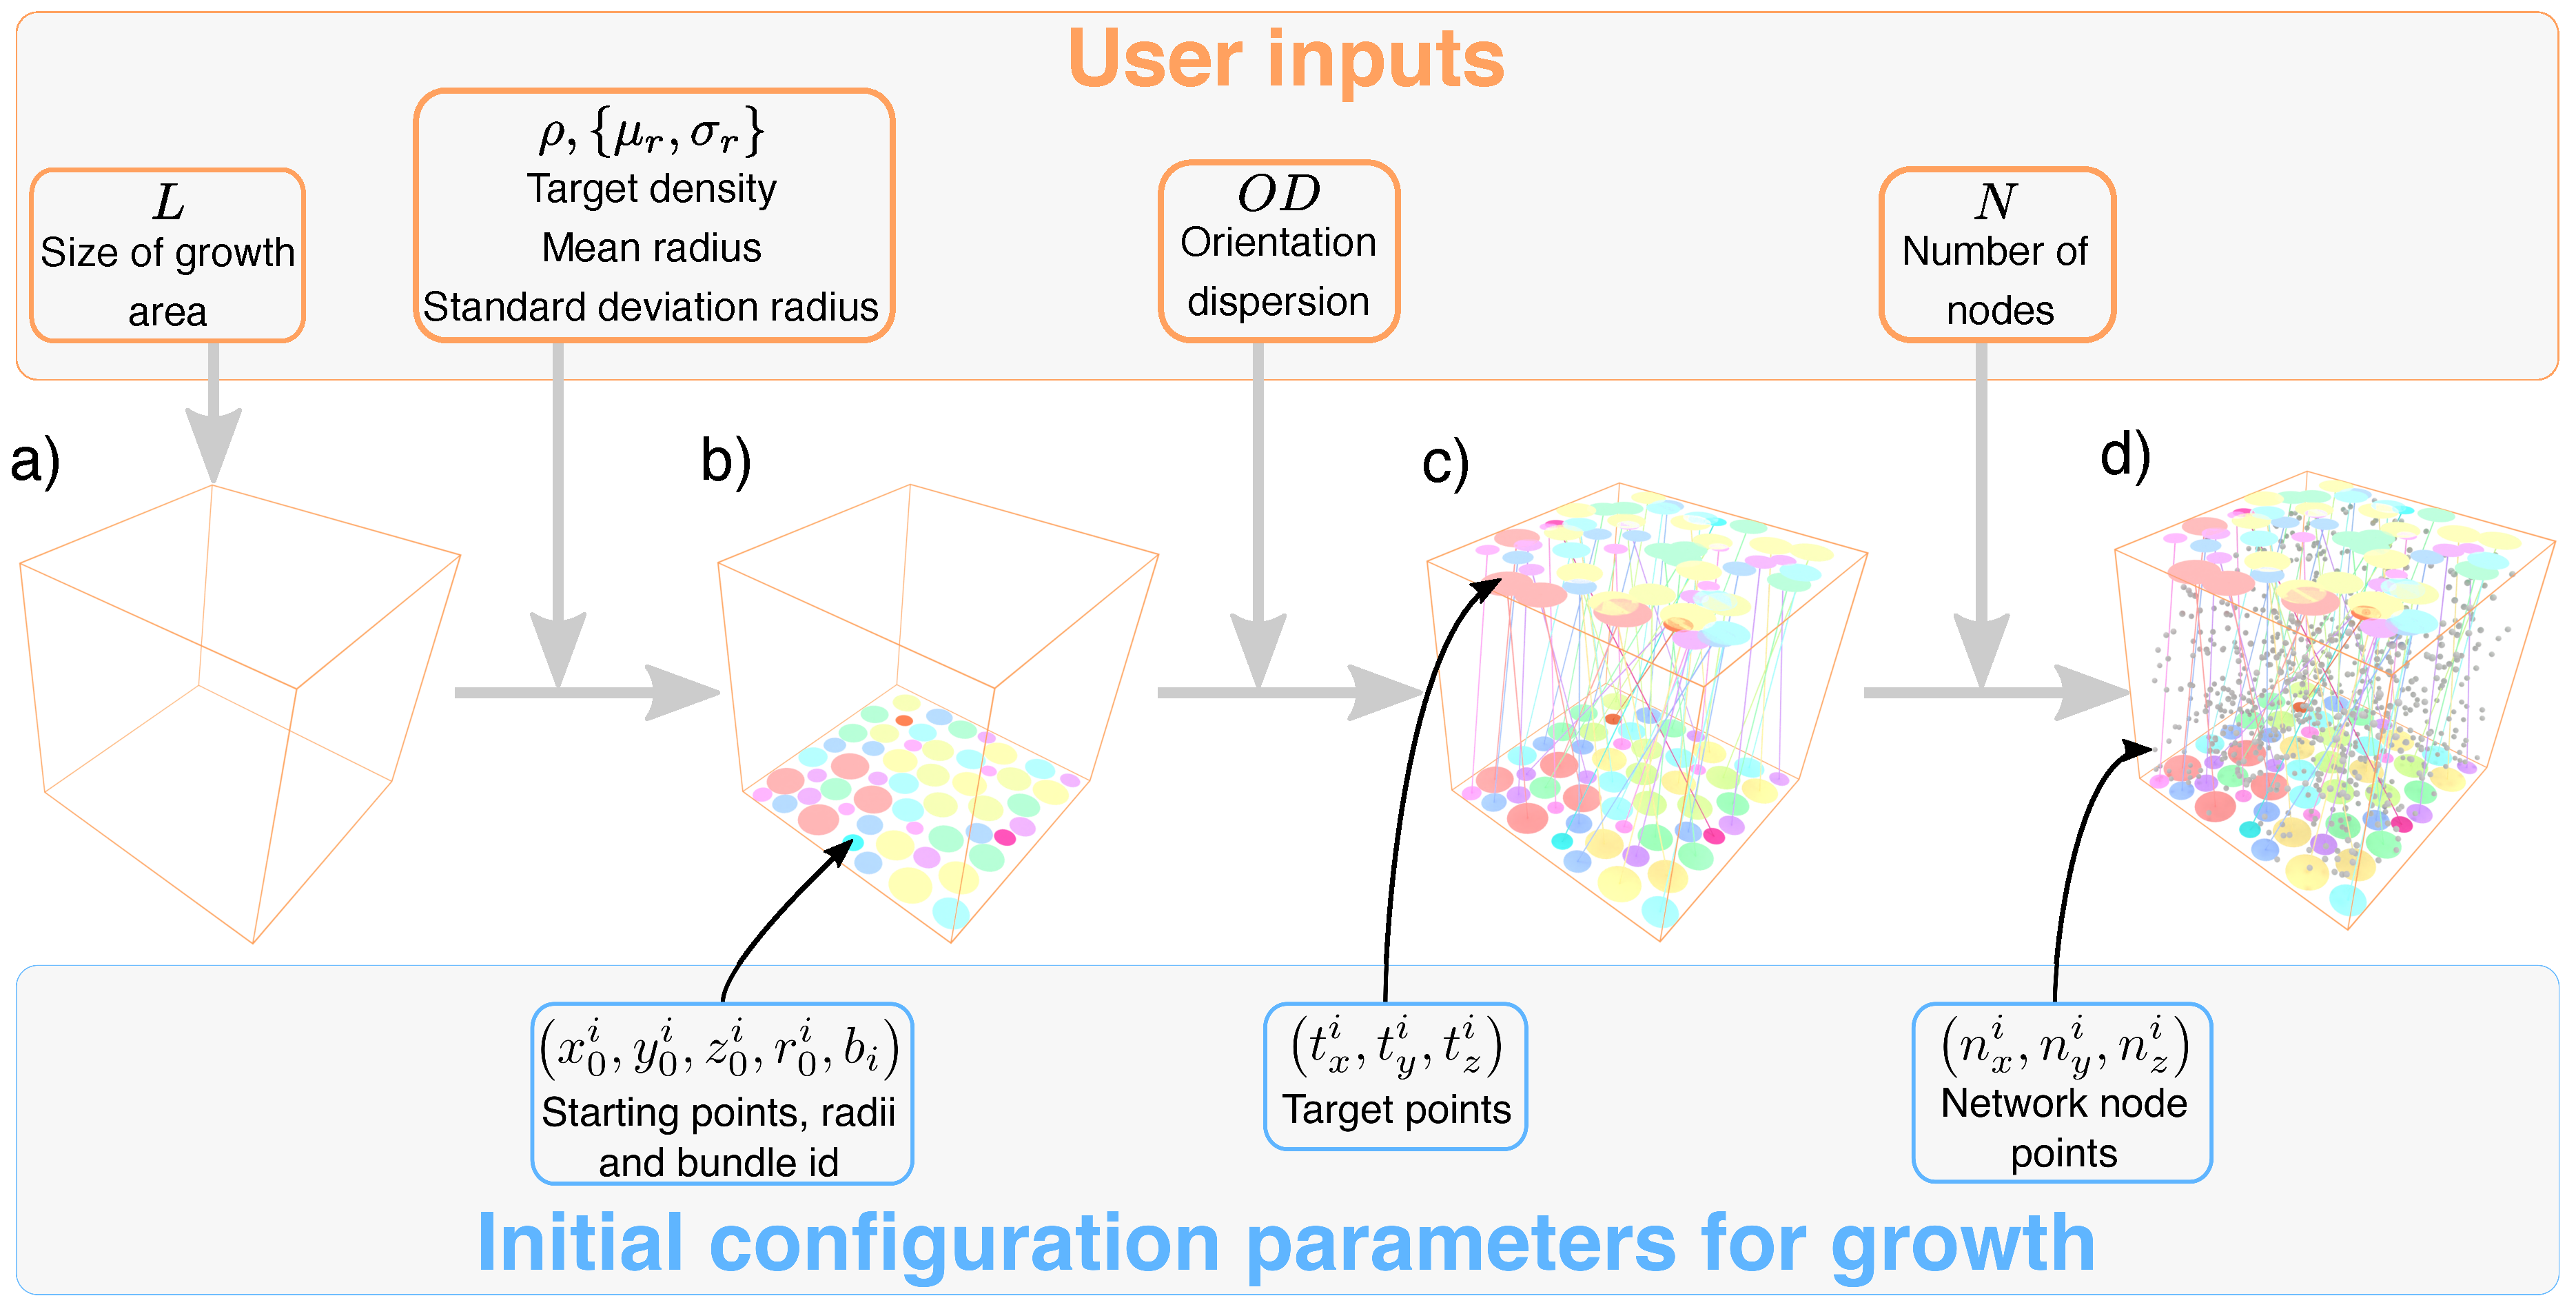
\includegraphics[width=\textwidth]{figures/config/method_inputs_only.eps}
  \caption[Inputs to the ConFiG algorithm]{Inputs to the ConFiG algorithm for the single bundle case. $L$ defines the size of the area of that the growth will take place in. The target density and fibre radius distribution govern the generation of starting points for each fibre by packing in 2D. Orientation dispersion parameters govern the generation of target points corresponding to each starting point. $N$ defines the number of nodes to use when generating the network. In the case of multiple bundles, starting and target points are generated for each bundle and then combined into the same space which is filled with nodes for the network. }
  \label{fig:config_inputs}
\end{figure}

First, Step 1 is broken down in to three substeps as outlined in \Cref{fig:config_inputs}:
\begin{description}
  \item [STEP 1.1] Generate fibre starting points (~\Cref{fig:config_inputs}a-b). To generate a starting point for each fibre to grow from, ConFiG packs circles with the desired diameter distribution up to the target density (defined in terms of the desired fibre volume fraction) in 2D, following the approach taken in \cite{Hall2009}.

  \item [STEP 1.2] Generate fibre target points (~\Cref{fig:config_inputs}c). To encode the desired orientation distribution, each fibre has a direction drawn from the target distribution which gives a target point for the fibre to grow towards. As a demonstration of the flexibility of the framework, in this work we use the Watson distribution \cite{Mardia2008} for isotropic dispersion and the elliptically symmetric angular Gaussian distribution \cite{Paine2018} for anisotropic orientation dispersion, however other orientation distributions can be defined according to the user’s needs.

  \item [STEP 1.3] Generate growth nodes (~\Cref{fig:config_inputs}d). ConFiG uses a set of pseudorandomly placed points (nodes) to sample the space and encode which regions are occupied by existing fibres. This simplifies collision checking making growth more efficient than a direct collision detection approach involving growing each fibre one small step at a time and checking collisions with existing fibres \cite{Callaghan2019}.
\end{description}

\begin{figure}[h!]
  \centering
  \includegraphics[width=\textwidth]{figures/config/method_without_inputs1.eps}
  \caption[Overview of the ConFiG growth algorithm]{Overview of the basic growth algorithm in ConFiG. In this example, three fibres are shown with a growth network that only contains relevant nodes for the sake of visualisation.  From the set of nodes, a network is constructed using the Delaunay triangulation. Each fibre then grows from node to node, along any edge connected to the current node. The node moved to will be the node with the lowest cost. Once a fibre segment has grown, the network nodes are updated to store information about which nodes are occupied or near to an existing fibres. This contributes to the cost function for any future fibres, penalising moving to nodes too close to existing fibres.  It is not possible to move to any node now inside a fibre as indicated by the removal of this edges from the network (pairs of blue arrows show where this is happening). The next fibres grow, now avoiding existing fibres until all fibres have finished. See Supplementary Video 1 for an animation of this algorithm. }
  \label{fig:config_algorithm}
\end{figure}

Second, Step 2, the main growth algorithm, is broken down into a series of substeps as outlined in \Cref{fig:config_algorithm}:
\begin{description}
  \item [STEP 2.1] Create growth network (~\Cref{fig:config_algorithm}a\&b). In order to encode which nodes a fibre can move to from any other node, the growth nodes are connected using the Delaunay triangulation.

  \item [STEP 2.2] Grow one fibre step (~\Cref{fig:config_algorithm}c-e). Fibres grow one-by-one in a random order along this network towards their target points while avoiding existing fibres. During growth, a fibre must choose in which direction it should grow. This direction is chosen in ConFiG by following a cost function motivated by biological axonal guidance mechanisms (~\Cref{fig:config_algorithm}d), described in \Cref{sec:config_chemoattraction,sec:config_fasciculation}.

  \item [STEP 2.3] Update the network (~\Cref{fig:config_algorithm}f). The growth network is updated in order to store the information about the space this fibre is occupying so that future fibres can avoid it. The simplest way to do this is to store the minimum distance from each node in the network to any existing fibre as in \cite{Callaghan2019}. Additionally, another biologically motivated network updating strategy is described in \Cref{sec:config_dynam_growth}.

  \item [STEP 2.4] Repeat steps 2.2 and 2.3 until fibre reaches target (~\Cref{fig:config_algorithm}g). By default in ConFiG, each fibre will grow completely before the next one starts, meaning that step 5 only needs to be performed once the fibre has finished growing. If fibres are allowed to grow concurrently, step 5 must be performed after each growth step.

  \item [STEP 2.5] Repeat steps 2.2-2.4 for remaining fibres (~\Cref{fig:config_algorithm}h-i). As noted in \Cref{fig:config_algorithm} (e-h), as the network is updated, more and more nodes become inaccessible making the network sparser. This means that some fibres may reach a point from which they cannot grow any further and will become stuck. Biologically inspired mechanisms designed to address this point are described in \Cref{sec:config_fibre_collapse,sec:config_dynam_growth}.
\end{description}

Finally, Step 3, the meshing procedure, is briefly described below and in further detail in \Cref{sec:config_meshing}:
\begin{description}
  \item [STEP 3] Generate 3D fibre meshes. After the growth process, each fibre will be represented by a series of connected 3D points and corresponding diameters at each point. In order to simulate diffusion MRI signals, these fibre skeleta need to be turned into 3D meshes. ConFiG uses a meshing procedure designed to eliminate overlap between fibres.
\end{description}

The basic ConFiG growth algorithm described here is illustrated in \Cref{fig:config_algorithm}, with an animation of the algorithm in Supplementary Video 1. The remainder of this section outlines the biological process governing real axonal growth, and how these processes motivated the final implementation of the ConFiG algorithm.

\subsection{Biological motivation for ConFiG}
\label{sec:config_biol_motiv}
In nature, axons grow following chemical cues in their environment through various mechanisms which either attract or repel fibres to guide their growth \cite{Dent2011,Lowery2009,Mortimer2008,Polleux2010,Price2017,Rauch2013,Sakisaka2005}. In an attempt to emulate real axonal growth, mechanisms motivated by the following guidance processes have been integrated into ConFiG:
\begin{itemize}
  \item Chemoattraction – the process by which fibres are attracted to diffusible chemical cues in their environment \cite{Price2017,Mortimer2008}.
  \item Fibre collapse – a response to a chemorepulsive source whereby a fibre withdraws and regrows in a different direction \cite{Rauch2013}.
  \item Cell adhesion molecules – chemical signals on the surface of cells which guide axons that come into contact with them \cite{Sakisaka2005}.
  \item Fasciculation – the process by which multiple axons come together to form bundles \cite{Price2017,Smit2017}.
\end{itemize}
The following sections detail how mechanisms motivated by these biological processes are implemented in ConFiG while \Cref{fig:config_chemoattraction,fig:config_dynam_growth,fig:config_fasciculation} illustrate these biological processes alongside their ConFiG counterparts.

\subsubsection{Chemoattraction}
\label{sec:config_chemoattraction}
As mentioned in \Cref{sec:config-alg-overview}, as a fibre grows it must choose in which direction it will move. One of the main processes governing the guidance of real axons is chemotropism; a process by which axons respond to diffusible chemical cues in their environment. One key chemotropic mechanism is chemoattraction, in which fibres are attracted along a chemical gradient towards a target region \cite{Price2017}.

\begin{figure}
  \centering
  \includegraphics[width=\textwidth]{figures/config/biological_target+cam-01.png}
  \caption[Illustration of the chemoattraction process]{Illustration of two of the biological motivations and how they are implemented in ConFiG. a) Growth towards the target is enforced by means of a cost function encouraging growth towards the target point. b) Fibre collapse is implemented by allowing the fibre to move backwards if it reaches a node from which there are no viable steps. The biological figures are adapted from \cite{Price2017}}
  \label{fig:config_chemoattraction}
\end{figure}

To approximate this chemoattractive mechanism, each fibre is encouraged to grow towards its target point (i.e. the target point acts like a chemoattractive source). From any node in the growth network, the fibre will move along an edge that takes it towards its target while avoiding existing fibres according to a cost function \cite{Callaghan2019}. The chemoattractive mechanism and its ConFiG counterpart are illustrated in \Cref{fig:config_chemoattraction}a.
From a starting node, $s$, the candidate nodes, $c$, that the fibre can move to are any nodes that share an edge with $s$. In addition to its position, each network node stores the maximum fibre diameter, $d_c$, that can be sustained at that node without intersecting another fibre. The fibre will move to a candidate node according to a cost function consisting of two terms; $l_t$, which penalises taking very large steps or moving away from the target point, $t$, and $l_d$, which penalises moving to a position where $d_c$ is low meaning that the fibre will have to shrink. The cost function for a fibre at a position, $s$, to move to a candidate node, $c$, given a target point, $t$, is (Callaghan et al., 2019)
\begin{align}
  l &= l_t+fl_d  \,,\label{eq:original_cost}\\
      \mathrm{where}\nonumber\\
  l_t &=  \frac{1}{2} \cdot \frac{\|s-c\|}{1+ \|s-c\|} \cdot \left(1- \frac{\left(\left(c-s\right) \cdot \left(t-s\right)\right)}{\|c-s\|\|t-s\|}\right)\,, \label{eq:original_lt}\\
  l_d &=\mathrm{max}\left(0, \frac{1}{d_0} \left(d_0 - d_c \right)\right) \,. \label{eq:original_ld}
\end{align}
Here, $d_0$ is the target diameter of the fibre and $f$ is a weighting factor between the two terms. In this work, $f$ is fixed to 0.2 to more strongly weight growth towards the target.

The next node for a fibre will be the candidate node which has the lowest cost according to Equation (1). This method of finding a path through the triangulation by choosing the lowest cost node at each position amounts to a greedy best-first pathfinding approach with a heuristic given by Equation (1).

Growing fibres along the network using just this chemoattractive mechanism is the minimal implementation of ConFiG that will generate substrates to try and meet the morphological inputs. There are some limitations to this minimal approach however; the greedy growth and the sparse sampling of the space means that fibres can grow into regions from which they cannot grow further and become stuck. Additionally, in this approach, fibres grow independently of one another, whereas real fibres grow forming bundles in the process known as fasciculation.

\Cref{sec:config_fibre_collapse,sec:config_dynam_growth,sec:config_fasciculation} describe further mechanisms which were added to enable ConFiG to address these limitations in order to meet more complex morphological priors (e.g. high density and orientation dispersion together).

\subsubsection{Fibre Collapse}
\label{sec:config_fibre_collapse}
As mentioned in \Cref{sec:config_biol_motiv}, in ConFiG a fibre can become stuck when there are no possible next steps because all neighbouring nodes are inaccessible. In an attempt to ameliorate this a process mimicking fibre collapse was implemented, illustrated in \Cref{fig:config_chemoattraction}b.

In ConFiG fibre collapse, the fibre will move back by an initial distance, $g_0$, and regrow from there avoiding any nodes in the route it took previously. If the fibre becomes stuck again, it will move back by a further distance, $g_0+ \delta$, where $\delta$ is the additional distance to step back. This process is repeated until the fibre reaches the target or gets stuck a user-defined maximum number of times. In this work, $g_0=\SI{2}{\micro\metre}$  and $\delta=\SI{5}{\micro\metre}$ in an approximation of the biological fibre collapse process investigated by Rauch et al. \cite{Rauch2013} who show fibres collapsing up to \SI{25}{\micro\metre} back towards the soma. The maximum number of steps back is set to 5, meaning that the maximum step back is \SI{27}{\micro\metre}, in line with real fibres. If there is no possible route after 5 attempts then the fibre will stop growing and will be removed from the phantom. This process of removing stuck fibres means that the resulting substrate may not always have the same density as the input desired fibre density.

\subsubsection{Dynamic Growth Network}
\label{sec:config_dynam_growth}

\begin{figure}
  \centering
  \includegraphics[width=0.8\textwidth]{figures/config/biological_cam.png}
  \caption[Illustration of the contact guidance mechanism]{Illustration of the contact guidance axonal growth mechanism and the dynamic growth network implemented in ConFiG. The dynamic growth network is implemented as a set of points added around each fibre after growth, enable future fibres to more easily grow along/around existing fibres.}
  \label{fig:config_dynam_growth}
\end{figure}

In the preliminary implementation of ConFiG \cite{Callaghan2019}, the network nodes were initialised pseudorandomly within the growth region and once initialised, the growth network was static, meaning that the nodes and edges of the network were fixed. This limited the growth to the specific instantiation of the network and it could not adapt to where fibres were once they had grown. Furthermore, as illustrated in \Cref{fig:config_algorithm}, as fibres grow, many nodes become inaccessible due to being within fibres meaning that the network becomes gradually sparser.

A dynamic growth network was implemented to ameliorate these effects. Now, once a fibre has reached the target, a number of nodes, $N_{added}$, are generated around the path of the fibre. This gives a denser sampling of the space in regions in which fibres exist and serves to give subsequent fibres more nodes to use to grow along or around that fibre, helping to increase the achievable density by limiting the number of fibres which get stuck. In this work, where the dynamic network is used, $N_{added}=2500$.

This is also loosely motivated by the contact guidance mechanism in which axons are attracted to or repelled by chemical cues on the surface of other cells, known as cell adhesion molecules (CAMs). Here, the added points act like CAMs meaning that a future fibre which grows can use these points near to the fibre to grow around or along it as if it were following contact guidance cues. \Cref{fig:config_dynam_growth} shows how CAMs work in biological axonal growth alongside the ConFiG dynamic network, illustrating the parallels between the two.

\subsubsection{Axon Fasciculation}
\label{sec:config_fasciculation}

\begin{figure}
  \centering
  \includegraphics[width=0.5\textwidth]{figures/config/biological_fasciculate.png}
  \caption[Illustraction of the fasciculation process]{Illustration of how the labelled pathway hypothesis is expected to work in biology and its ConFiG counterpart. Fasciculation is implemented using the cost function term in Eq. 1 which means that fibres in the same bundle are encouraged to stay close to one another.}
  \label{fig:config_fasciculation}
\end{figure}

One particular role CAMs play is in axon fasciculation, the process in which axons follow a so-called pioneer axon closely, forming a bundle \cite{Price2017,Sakisaka2005}. To mimic the process of axon fasciculation, the term in the cost function penalising moving into regions in which the fibre had to shrink, $l_d$ (Equation (3)), was altered to be conditional on which fibre bundle is closest.

A fibre, $f$, with a target diameter, $d_0$, moving to a candidate node, $c$, which has a maximum sustainable diameter $d_c$ will now have $l_d$ given by:
\begin{equation}
  \label{eq:updated_ld}
  l_d = \begin{cases}
    \max\left(0, \frac{1}{d_0} \left(d_0 - d_c\right)\right) & \text{if } b_c \neq b_f \\
    \mathrm{abs}\left(\frac{1}{d_0} \left(d_0 - d_c\right)\right) & \text{if } b_c = b_f
    \end{cases}
\end{equation}

Where $b_f$ is an index identifying the bundle that fibre $f$ belongs to and $b_c$ is the index of the bundle that is closest to $c$ (i.e. the index of the bundle of the fibre that set $d_c$). This means that when $c$ is closest to the same bundle as $f$, the cost function penalises moving away from that bundle as well as shrinkage, whereas when the bundles differ, it only penalises shrinkage.

This new form of the cost function encourages fibres of the same bundle to stick together while still avoiding fibres of different bundles, inspired by the labelled pathway hypothesis, which states that axons join different fascicles based on different CAMs expressed on the fibres \cite{Price2017}. In this case, bundle indices $b_c$ and $b_f$ act like different identifying CAMs. \Cref{fig:config_fasciculation} shows how this fasciculation process is expected to happen in biology alongside how the improved cost function encourages a similar process in ConFiG.

\subsubsection{Global Optimisation}
\label{sec:config_global_optimisation}
Since the growth of fibres in ConFiG takes place on a discrete network of points, the final positions of fibre nodes may be suboptimal for achieving the maximum density. In other words, certain fibres’ nodes may be closer to other fibres than they would ideally be in order to reach their target diameter (i.e. the fibre has had to shrink its diameter at that node).

To mitigate against this, a global optimisation step was added at the end of the growth in a procedure similar to MEDUSA \cite{Ginsburger2019}. For each point, $i$, that is part of a fibre, its nearest $n$ neighbours $(j \in NN(i))$ from other fibres are found; in this work $n=10$. The distance to all of the neighbours is found and the point’s position is updated from these distances according to the update vector, $\vec{u}_i$
\begin{equation}
  \label{eq:global_opt_update_vec}
\vec{u}_i= \sum_{j \in NN(i)} D(i,j) \cdot \left(\vec{p}_i - \vec{p}_j\right) \,,
\end{equation}
where $\vec{p}_i$ and $\vec{p}_j$ are the locations of point $i$ and $j$. $D(i,j)$ is the function determining whether the interaction is repulsive or attractive:
\begin{equation}
  \label{eq:global_opt_Dij}
  D(i, j) = \mathrm{sgn}\left(r_i + r_j - \|\vec{p}_i - \vec{p}_j\|\right) \,.
\end{equation}

Here, $\mathrm{sgn}$ is the signum function and $r_i$ and $r_j$ are the target radii of point $i$ and $j$. The sum of these radii is the desired distance between the points since that means the fibres are just touching. $D(i,j)$ imposes that the force is repulsive if the points are closer together than the desired radius and attractive if they are further apart. The update vector is scaled such that if $\|\vec{u}_i\| > 0.2r_i$, the update vector is rescaled so that $\|\vec{u}_i\|=0.2r_i$. This acts to prevent the update vector from becoming very large.

There is some biological evidence that this kind of interaction between fibres is important in the fasciculation process. The fasciculation process described in \Cref{sec:config_fasciculation} relies on CAMs detected at the tip of a growing axon, however some studies provide evidence for fasciculation through interactions along axon shafts, known as zippering \cite{Barry2010,Smit2017,Voyiadjis2011}. In zippering, nearby axon shafts attract one another to form more closely packed fascicles, which is a similar process to the global optimisation process in ConFiG.

\subsubsection{Creation of 3D meshes}
\label{sec:config_meshing}

\begin{figure}
  \centering
  \includegraphics[width=0.8\textwidth]{figures/config/METABALL_fig.png}
  \caption[ConFiG meshing procedure]{Demonstration of the meshing procedure in ConFiG. The first fibre is created using metaballs to create a smooth surface. The second, and following fibres will be created using negative metaballs for any fibres that intersect in order to deform around them. Note that in practice, more spheres will be much more closely placed along the skeleton to create a smoother surface}
  \label{fig:config_meshing}
\end{figure}

As mentioned in \Cref{sec:config-alg-overview}, following the growth process ConFiG fibres will be represented by a series of connected points and corresponding radii. To convert these skeleta into 3D meshes, the ConFiG meshing procedure uses Blender (\url{https://blender.org}) and is built on the SWC mesher addon (\url{https://github.com/mcellteam/swc_mesher}).

ConFiG meshes are constructed using Blender metaballs, an implicit surface representation which is the isosurface of a function; typically a function analogous to the electric potential from a point charge. When two metaballs come close to one another, the fields combine and the surfaces will merge to form a smooth surface. By placing a series of metaballs along the skeleton of each fibre, a smooth surface is formed for each fibre one-by-one as shown in \Cref{fig:config_meshing}a. Supplementary Figure 1 demonstrates that the ConFiG meshing procedure does not impact the diffusion dynamics compared to a straight cylinder.

When fibres are densely packed, the surfaces from neighbouring fibres may overlap. To account for this, a meshing procedure was developed in which fibres can deform around nearby fibres to avoid overlap. The metaball surface for one fibre is created as described above. This surface is then turned into a triangulated mesh, however the metaballs are retained. The metaball potential is then turned negative, meaning that rather than merging with any future nearby metaball surfaces, it will repel them, as shown in \Cref{fig:config_meshing}b. This means that subsequent fibres which are meshed very close to, or overlapping with, existing fibres will deform organically to resolve the intersection, thus creating a series of completely non-intersecting fibre meshes which can be used by the dMRI simulator.

\subsection{Summary of ConFiG input parameters}
\label{sec:config_summary_of_input}
Table 1 summarises the key parameters that govern the generation of ConFiG phantoms. Parameters are split into those which define the target microstructural morphology and those which define the instantiation of the growth algorithm. For each parameter, the theoretical range is reported alongside the practical range that has been tested so far. This is due to stochastic nature of the algorithm and the interdependence of the parameters. For instance a very large substrate is possible if very large fibres are chosen, but likely impossible with very small fibres since this will require a very large number of fibres and run into memory limitations.

\section{Experiments}
\label{sec:config_experiments}
In order to assess the performance of ConFiG, a range of experiments were performed. The first set of experiments were performed in order to explore the impact of each of the biologically inspired growth mechanisms. Another set of experiments aimed to show that ConFiG is able to generate substrates with realistic microstructure by comparing generated substrates with real tissue. Additionally, the relationship between the user-specified target morphology and the final output morphology was investigated by comparing resulting phantoms to their inputs (target density and orientation distribution). Finally, a simulation experiment was performed to assess how well ConFiG phantoms can be used to generate realistic diffusion MRI data. The rest of this section outlines these experiments.

\subsection{Testing the performance of ConFiG}
\label{sec:config_test_perf}
In order to test how each of the biological mechanisms proposed in \Cref{sec:config_methods} impacted on the resulting phantoms, an experiment was devised to measure how phantoms changed when each mechanism was introduced. Four scenarios of interest were generated using several variants of the ConFiG algorithm that included these mechanisms either one at a time or all at once, attempting to grow phantoms as densely as possible:
\begin{itemize}
  \item one bundle of parallel fibres, target density 75\%
  \item one bundle with Watson distributed fibres $(\kappa=8)$, target density 75\%
  \item two perpendicular crossing bundles, intra-bundle target density 40\%
  \item three mutually perpendicular crossing bundles, intra-bundle target density 30\%
\end{itemize}
These target densities were chosen to ensure that the centre of the phantom (i.e. the crossing region for crossed bundles) had a high target density whilst ensuring that each bundle had a reasonable number of fibres to begin with (>50).

The ConFiG variants were tested by generating phantoms for each of the scenarios starting with the same initial conditions. Each phantom was generated 5 times with a different random seed and results averaged across the seeds.

To investigate the impact of the biological mechanisms on dMRI simulation, a comparison was made between real dMRI signals and simulations from ConFiG phantoms. The NODDI model \cite{Zhang2012} was fitted to a WM ROI in the corpus callosum of a Human Connectome Project (HCP) \cite{VanEssen2012} subject to provide sensible input parameters (target fibre density and orientation dispersion) for ConFiG to generate phantoms. We generated phantoms using the two extreme cases: the minimal growth case only using chemoattraction, and the complete ConFiG algorithm using all mechanisms. Whilst the random nature of ConFiG means that the resulting phantom will not have morphology exactly matching the input parameters, this approach ensured that the phantoms were reasonable for this proof of concept experiment.

The dMRI signal was simulated in the phantoms using Camino \cite{Cook2006,Hall2009} with identical simulation conditions in both cases and the measurement scheme corresponding to the HCP dMRI sequence \cite{Sotiropoulos2013a}. An important consideration when performing dMRI simulations is the size of the substrate relative to the diffusion length. The phantom should be large enough that it is bigger than the diffusion length, but not so large as to require excessive computational resources. Owing to the relatively long diffusion time (\SI{43}{\milli\second}) in the HCP sequence, phantoms were extended with reflected copies \cite{Lee2019a,Fieremans2018} to increase their effective size relative to the diffusion length scale.

All dMRI simulations in this work used a bulk diffusivity $D=\SI{2.0}{\micro\metre\squared\per\milli\second}$ in agreement with values used in similar Monte Carlo simulations \cite{Hall2009,Nilsson2009,Rensonnet2017} with $10^5$ spins and $2000$ timesteps. Standard Camino periodic boundaries were used \cite{Hall2009}, with dMRI signal was generated from a central region 75\% the size of the total phantom to avoid boundary effects \cite{Panagiotaki2010}.

\subsection{Microstructural measures}
\label{sec:config_micr_meas}

\begin{figure}
  \centering
  \includegraphics[width=\textwidth]{figures/config/centre_line_extraction-01.png}
  \caption[Mesh centreline extraction]{Centre line extraction of fibres. Each fibre was sliced N times along the z-axis, connecting the centre of mass of each slice to create the points in the centre line. This line could then be optionally smoothed according the diffusion time coarse graining effect, as in \cite{Lee2019b}}
  \label{fig:config_micro_centreline}
\end{figure}

In order to test how realistic the microstructure generated using ConFiG is, microstructural measurements of diameter distribution and orientation distribution were calculated using methods to be comparable with previous studies on ex-vivo tissue \cite{Abdollahzadeh2019,Lee2019b}.

A centre line is generated from each of the fibre meshes by aligning the ends of each fibre with the z-axis and connecting the centre of mass of 100 equidistant slices through each fibre, following the approach taken by Lee et al., \cite{Lee2019b}. This is illustrated in \Cref{fig:config_micro_centreline}.

Each segment in this centre line could then be used to assess the microstructure of the phantom. The direction of each segment was used to assess the orientation distribution of the phantom, illustrated in \Cref{fig:config_micro_OD}. Following the approach of Lee et al., \cite{Lee2019b}, the direction of each segment was projected onto the surface of a triangulated unit sphere \cite{Womersley2018}. For each triangle, the number of segments pointing in that direction was used to colour the triangle to visualise the orientation distribution.

\begin{figure}
  \centering
  \includegraphics[width=\textwidth]{figures/config/od_calculation-01_sym_whitebg.png}
  \caption[Orientation distribution extraction from microstructure]{Orientation distribution calculation. Each segment of a fibre was projected onto the surface of a triangulated sphere, here illustrated with a sectioned circle. For each section in the sphere, the number of fibre segments going through that section was used to colour and/or raise the surface to visualise the orientation distribution. Since the diffusion process is symmetric about the origin, each fibre segment was projected onto the sphere forwards and backwards.}
  \label{fig:config_micro_OD}
\end{figure}

\begin{figure}
  \centering
  \includegraphics[width=\textwidth]{figures/config/diam_calculation-01.png}
  \caption[Diameter distribution extraction from microstructure]{Calculation of the diameter distribution. A slice is taken through each fibre perpendicular to every segment in the centre line. The area of each of these slices is used to find a circle equivalent radius or diameter using $A = \pi r^2$. }
  \label{fig:config_micro_diam}
\end{figure}

A second approach was devised to better visualise orientation distributions in 3D to aid differentiation of crossing bundles and antipodal symmetry. In this approach each vertex was raised above the surface of the sphere proportionally to the number of segments pointing in its direction as illustrated in \Cref{fig:config_micro_OD}.

To measure the diameter profile along fibres, the direction of each segment gave the normal to a plane used to cut the fibre using Boolean intersection to give a cross section of each fibre at each segment. The diameter profile along the axon was generated by calculating the equivalent diameter of a circle with the same area as the fibre cross section. This process is illustrated in \Cref{fig:config_micro_diam}.

\subsection{Virtual Histology}
\label{sec:confg_virtual_histology}
Virtual histological slices were generated to compare ConFiG substrates to real white matter analysed using histology. Histological slices were found by calculating the Boolean intersection of a cutting plane with the generated fibre meshes using Blender (\url{https://blender.org}). A myelin sheath was added to the fibres when generating virtual histology for visualisation purposes.  Virtual histological images were rendered with a resolution of \SI{5 x 5 x 100}{\nano\metre}, chosen to be comparable to real histological white matter measurements \cite{Abdollahzadeh2019,Lee2019b}.

In order to compare ConFiG virtual histology to real histology, virtual histological slices were rendered in binary black and white to compare against intra-axonal segmentations from \cite{Lee2019b}. Slices from real histology, ConFiG phantoms and a parallel cylinder phantom were processed using the MorphoLibJ plugin for ImageJ \cite{Rueden2017,Legland2016,Schindelin2012,Schneider2012} to extract morphological features: circularity ($4\pi$ × Area/Perimeter$^2$), convexity (Area of shape/Area of convex hull), eccentricity of fitted ellipse and Area/$\pi r_{max}^2$ for each axon. Axons touching the edge of the image were removed since truncation from the image edge would skew these microstructural metrics.

\subsection{Relationship between input and output morphology}
\label{sec:config_input_output_rel}
As mentioned in \Cref{sec:config_methods}, the nature of the ConFiG growth algorithm means that the microstructural morphology of the phantoms may not match the user input. Some fibres may become stuck and fibres cannot typically grow in a straight line, affecting the density and orientation distribution.

To investigate this, we generated a series of ConFiG phantoms with Watson distributed orientation dispersion with $\kappa=[8,10,15,20,30,50,100]$ and target density, $\rho = 75$\%. The target density of 75\% is chosen as this is the upper limit of what is achievable empirically and towards the higher end of expected axonal volume fraction. Additionally, with 75\% achieved, lower densities can be generated easily, either by running ConFiG in full, or simply by removing or shrinking fibres.

The mean and standard deviation of the angle from $z$, $\mu_\theta$ and $\sigma_\theta$ respectively, for each $\kappa$ was calculated by taking $10000$ samples from the Watson distribution and this was compared to $\mu_\theta$ and $\sigma_\theta$ of the ConFiG fibres. Additionally, the density of the ConFiG phantoms was compared to the target density of 75\%. Each phantom was generated in a \SI{20 x 20 x 20}{\micro\metre} region, using \num{2.5e6} nodes in the growth network.

\subsection{Diffusion MRI simulation}
\label{sec:config_diffusion_sim}
To qualitatively verify that the simulated diffusion MRI signals from ConFiG phantoms are realistic, simulated signals from ConFiG phantoms were compared to real HCP data \cite{Sotiropoulos2013a,VanEssen2012}.

In the real data, the fibre orientation distribution (FOD) was fit in each voxel using constrained spherical deconvolution in MRTrix \cite{Tournier2019,Tournier2007}. Voxels were selected in regions of interest in the midbody of the corpus callosum (CC), internal capsule (IC), regions in which a single bundle of fibres is found from the FOD. A third voxel was selected in which three crossing fibre populations were found from visual inspection of the FOD (TC).

In each voxel, the diffusion tensor was fit to the signal and the principal eigenvector used to define a major direction of diffusion in the voxel, $n$. From this, the normalised diffusion weighted signal was plotted against $|n\cdot G|$, where $G$ is the gradient direction. Additionally, the direction averaged signal was calculated for each b-shell.

To attempt to generate representative microstructure for each voxel using ConFiG, the NODDI model \cite{Zhang2012} was fitted to the average signal to give some initial parameters for ConFiG. Most importantly, the value of $\kappa$ for the Watson distribution \cite{Mardia2008} estimated using NODDI was used to initialise the orientation dispersion in the ConFiG phantoms used to represent CC ($\kappa=6.2$) and IC $(\kappa=5.5)$ regions. To represent the TC voxel, a phantom generated using three mutually perpendicular crossing bundles was used.

ConFiG phantoms were grown using these initial conditions and the diffusion MRI signal simulated using the Camino Monte Carlo diffusion MRI simulator \cite{Hall2009}. For each phantom, the same processing as with the real data was performed, finding the direction dependent and direction averaged signal per b-shell.

\section{Results}
\label{sec:config_results}

\subsection{Impact of biological mechanisms}
\label{sec:config_result_impact_of_mechanisms}

\begin{figure}
  \centering
  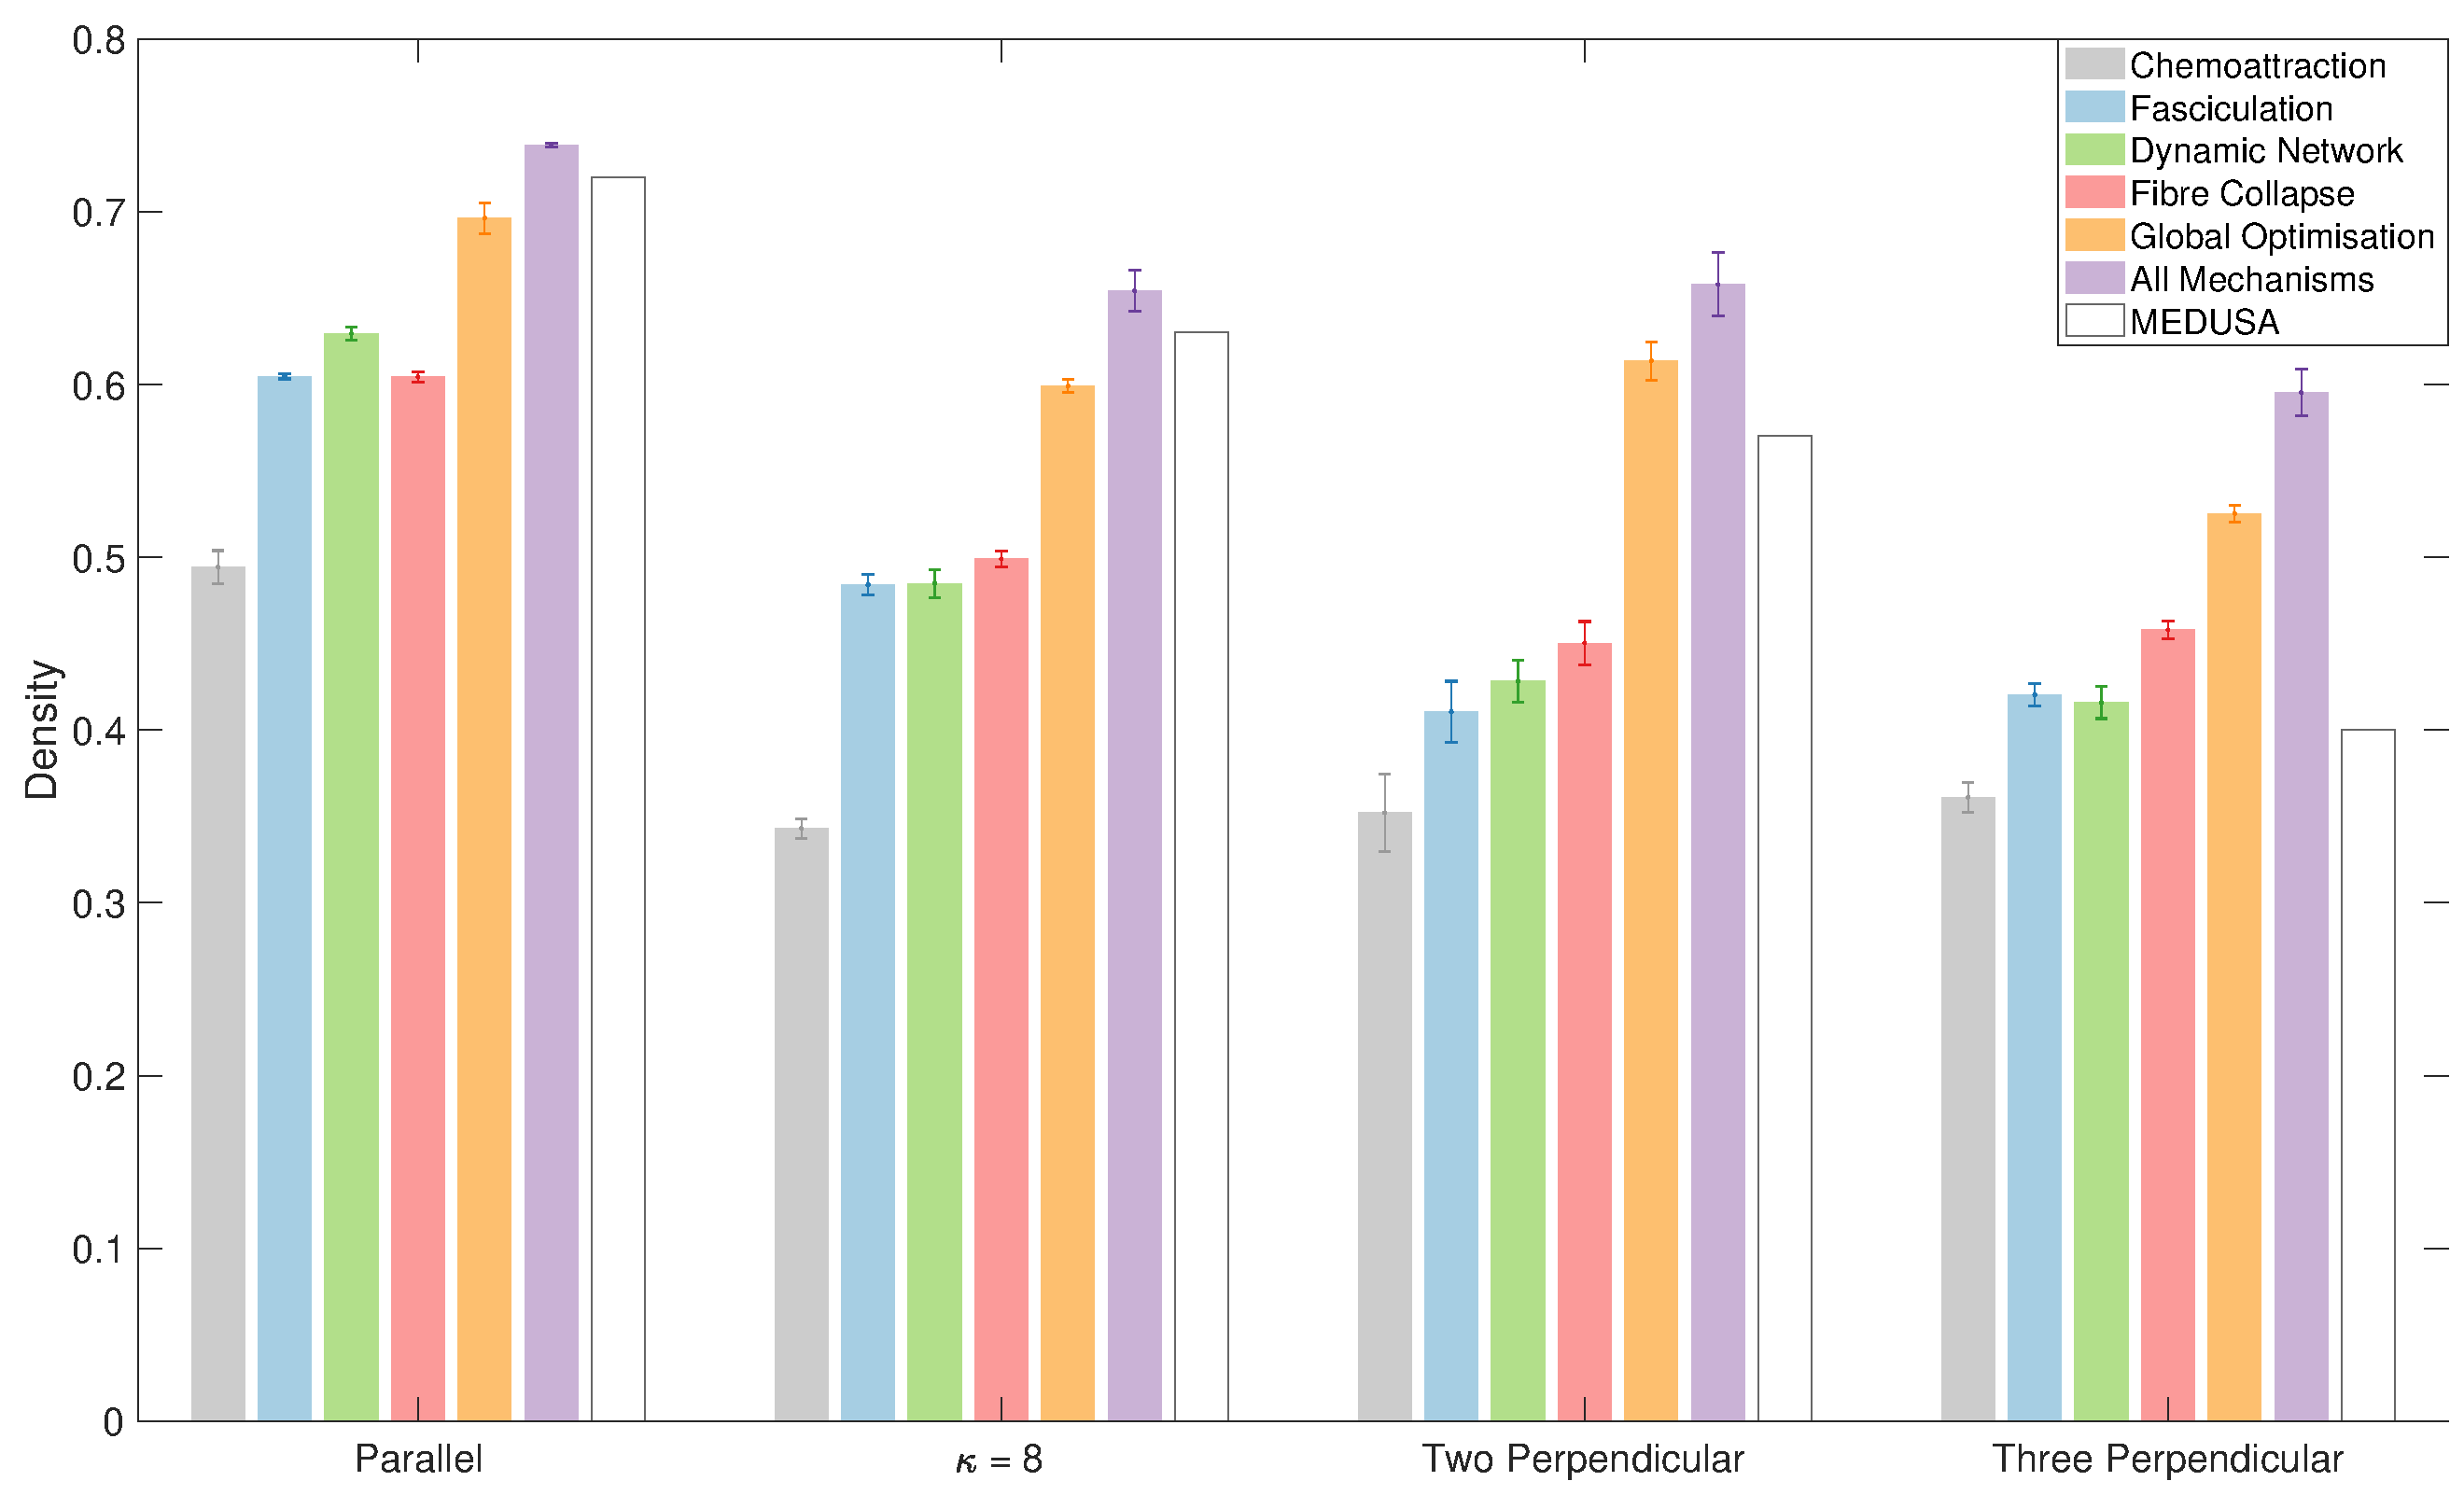
\includegraphics[width=\textwidth]{figures/config/improvements_wfascicle_tight.eps}
  \caption[Impact of biological mechanisms in ConFiG]{Demonstration of the impact of each biological growth mechanism on the density achievable with ConFiG. Each bar shows the mean density for each proposed mechanism, error bars show $\pm$ standard error on the mean. MEDUSA values are estimated from Fig. 14 in Ginsberger et al. (Ginsburger et al., 2019).}
  \label{fig:config_res_improvements}
\end{figure}

Each of the proposed biological mechanisms enabled ConFiG to generate phantoms with increased density over the minimal case of chemoattraction only, as is shown in \Cref{fig:config_res_improvements}. Global optimisation resulted in the largest improvement, 17-24\%, consistently giving a large improvement. Other improvements performed better for specific phantom configurations. For instance, fasciculation and the dynamic network produced only modest improvements in crossing fibre configurations (4-6\%), but performed well in the single bundle cases (11-14\%). Fibre collapse was particularly effective in the three perpendicular case, offering 10\% improvement.

\begin{figure}
  \centering
  \includegraphics[width=\textwidth]{figures/config/improvements_virthist.png}
  \caption[Impact of biological mechanisms on virtual histology]{Virtual histology demonstrating the impact of biologically inspired mechanism on the final phantom created for one of the parallel phantoms tested. This visually demonstrates the improvement in density. Leftmost image shows the phantom generated with all mechanisms in 3D and the cutting plane used to produce the virtual histology.  }
  \label{fig:config_res_improvements_virthist}
\end{figure}

\begin{figure}
  \centering
  \includegraphics[width=\textwidth]{figures/config/improvement_3drender.png}
  \caption[Impact of biological mechanisms on 3D phantoms]{Demonstration of the improvement in density achieved when using all mechanisms in ConFiG compared to the minimal implementation using only chemoattraction. Colours chosen to match \Cref{fig:config_res_improvements}. }
  \label{fig:config_res_improvements_3d}
\end{figure}

\begin{figure}
  \centering
  \includegraphics[width=\textwidth]{figures/config/hcp_old_vs_new_figure_whitebg.png}
  \caption[Impact of improvements on simulated dMRI signal]{Left: Direction averaged signal attenuation for real HCP data (± standard deviation over ROI) and simulated data from the minimal ConFiG implementation using only chemoattraction and using all growth mechanisms ConFiG showing that ConFiG can produce realistic dMRI signals. Right: The original and improved ConFiG phantoms used to generate the signal on the left. Simulations performed with $10^5$ spins, 2000 timesteps and HCP measurement scheme (Stamatios N. Sotiropoulos et al., 2013). Diffusivity set to $2.0microm ^2/ms$ , chosen to be consistent with previously reported values (Hall and Alexander, 2009; Nilsson et al., 2009; Rensonnet et al., 2017).  }
  \label{fig:config_res_improvements_sig}
\end{figure}

When combining all of the proposed mechanisms together, the achievable density is higher than any of the improvements individually. This improved performance is comparable to the state of the art, MEDUSA \cite{Ginsburger2019}, with particularly good performance relative to MEDUSA in the crossing fibre configurations.

This improvement in density can be appreciated visually in \Cref{fig:config_res_improvements_virthist} which demonstrates virtual histology of a parallel fibre phantom for each of the mechanisms. Additionally, \Cref{fig:config_res_improvements_3d} visually shows the difference in density of the phantoms in 3D between the minimal case of chemoattraction and all biological mechanism for each fibre configuration.

The improvement in the density of phantoms leads to a much more realistic simulated diffusion MRI signal as demonstrated in \Cref{fig:config_res_improvements_sig}. The root mean square error to the real data is reduced by 10 times when using improved ConFiG.

\subsection{Microstructural measures and virtual histology}
\label{sec:config_result_micro_meas}

\begin{figure}
  \centering
  \includegraphics[width=\textwidth]{figures/config/virthist1_wbox_whitebg.png}
  \caption[Comparison of real and virtual histology]{Comparison of real  and virtual histology. A) Light microscopy of rat ventromedial WM in thoracic spinal cord. Reproduced from Baxi et al. 2015 (Baxi et al., 2015), scale bar 2microm. B) Two virtual histological slices from a ConFiG generated phantom. Phantoms are rendered to have similar col ours to electron microscopy studies. The exact contrast and fibre bundle configurations are different between the real and virtual tissues, but the general morphology of the myelinated axons are captured well using ConFiG as highlighted by corresponding boxes. Yellow and Blue: axons severely deformed between other axons. Red: Pockets of empty space forming. Green: Largely circular axon surrounded by other axons deforming around it. Scale bar 2microm.}
  \label{fig:config_res_real_vs_virt_hist}
\end{figure}

The microstructural morphology generated using ConFiG is comparable to results from real data as demonstrated in \Cref{fig:config_res_real_vs_virt_hist,fig:config_res_slice_wise_metrics,fig:config_res_diameter_dist,fig:config_res_OD}.~\Cref{fig:config_res_real_vs_virt_hist} demonstrates virtual histology of a ConFiG phantom alongside a real EM image from mouse corpus callosum \cite{Baxi2015}. The exact microstructural features, such as diameter distribution, as well as the EM contrast do not exactly match between ConFiG and the real data. However, ConFiG is able to capture the general morphology or real axons as highlighted in \Cref{fig:config_res_slice_wise_metrics,fig:config_res_diameter_dist}. In particular, ConFiG is able to capture complex fibre cross-sections such as in the case of fibres squashed into small spaces. This is the first model of white matter able to handle complex fibre cross-sections such as this to our knowledge.

ConFiG morphological metrics calculated slice-wise on the virtual histology correspond much more closely to real axons than the same metrics calculated for parallel cylinders, as shown in \Cref{fig:config_res_slice_wise_metrics}. While cylinders produce a delta function at one extreme of each metric, ConFiG phantoms produce much closer distributions to the real data. Supplementary Figure 2 shows each of these slices coloured by their morphological metrics.

\begin{figure}
  \centering
  \includegraphics[width=\textwidth]{figures/config/slice_wise_metrics_whitebg.png}
  \caption[Slice-wise microstructural measurements]{Slice wise morphological metrics calculated for real axons, ConFiG phantoms and parallel cylinders. Across each of the metrics, ConFiG produces much more realistic distributions than  the cylinder phantom. Some of the cylinders have a non-zero eccentricity, but this arises since the metrics are calculated from binary images where the pixelated circles may appear to not be perfectly circular.}
  \label{fig:config_res_slice_wise_metrics}
\end{figure}

\begin{figure}
  \centering
  \includegraphics[width=\textwidth]{figures/config/diameter_dist_NEW_whitebg.png}
  \caption[Diameter distributions of real and ConFiG axons]{a) Along fibre diameter variation in ex vivo mouse corpus callosum, reproduced from (Lee et al., 2019) compared to along axis diameter variation in the phantom inset demonstrating the ability of ConFiG to generate realistic microstructure. b) Histograms of the inner diameter of axons from (Lee et al., 2019) and diameter of ConFiG axons. c) Coefficient of variation along axons for real and ConFiG axons and d) Three example fibres reconstructed from the EM data used by Lee et al. to make a). d) Three example ConFiG fibres selected for similarity to the EM examples }
  \label{fig:config_res_diameter_dist}
\end{figure}

The diameter distribution of a ConFiG substrate is compared to a reconstruction from real EM data \cite{Lee2019b} in \Cref{fig:config_res_diameter_dist}. ConFiG is able to capture the general profile of axonal variations well, with the overall shape of the diameter distribution matching well. The distribution of the coefficient of variation along ConFiG axons is slightly narrower with a smaller mean than real axons, though these discrepancies may be alleviated with a different choice of input parameters to ConFiG.

ConFiG is also able to generate orientation distributions comparable to real tissue as shown in \Cref{fig:config_res_OD}. The orientation dispersion is introduced to ConFiG phantoms using the elliptically symmetrical angular Gaussian \cite{Paine2018} to best approximate the EM data and also using isotropic Watson distributed directions to demonstrate the flexibility of ConFiG.

\begin{figure}
  \centering
  \includegraphics[width=\textwidth]{figures/config/OD_ESAG_wcolorbar_wiso_sym_whitebg.png}
  \caption[Orientation distributions from real WM and ConFiG phantoms]{Dispersion profiles for EM data and a series of numerical phantoms. Top row: EM data used to generate OD profile, reproduced from Lee et al. (Lee et al., 2019) and three ConFiG phantoms with one, two and three crossing bundles (each crossing bundle coloured a different shade of grey). Middle row: OD profile for real EM data and OD profiles corresponding to ConFiG phantoms above, generated using an elliptically symmetric dispersion. Bottom row: Three OD profiles generated from ConFiG phantoms generated using isotropic orientation dispersion. Colormap has units of steradians-1. }
  \label{fig:config_res_OD}
\end{figure}

\subsection{Relationship between input and output morphology}
\label{sec:config_result_input_output_rel}
The morphology of ConFiG phantoms matches the input morphology well, as shown in Table 2. Whilst the input and output $\mu_\theta$ and $\sigma_\theta$, do not match exactly, the values are close and increasing the input $\mu_\theta$ and $\sigma_\theta$ also increases the output $\mu_\theta$ and $\sigma_\theta$. Additionally, the output density generally matches the input target density well, achieving higher densities than MEDUSA for the same angular dispersion. Supplementary Table 1 shows the same experiment run with a target density of 60\% to demonstrate ConFiG’s performance at lower densities.

These phantoms took an average of 6 hours to grow plus an average of 20 minutes for the meshing and microstructural measurement procedure, using 9.4GB of RAM on average. These values give an estimate of the time taken to generate a typical ConFiG phantom, though it is strongly dependent on user inputs (number of nodes in the network etc.).

\subsection{Diffusion MRI simulation}
\label{sec:config_result_dmri_sim}
Simulated data from ConFiG substrates match real dMRI data well, as shown in \Cref{fig:config_res_dMRI}. The direction averaged signal matches well in each case, in particular, for the corpus callosum and three crossing phantoms, the simulated signal matches the real signal closely. The b = \SI{3}{\milli\second\per\micro\metre\squared} signal in the internal capsule and corpus callosum is lower in simulation than in real data. This is to be expected however because as $|n\cdot G|$ approaches 1, the signal reaches the noise floor and the noise-free simulations fall below the measured data. Supplementary Figure 3 shows the difference between the simulated and measured signal in 3D.

\begin{figure}
  \centering
  \includegraphics[width=\textwidth]{figures/config/hcp_vs_sim_new_review_2_whitebg.png}
  \caption[dMRI signals from HCP subject and ConFiG phantoms ]{Comparison of diffusion MRI simulations and real data from three different brain regions:  a) a voxel  in the midbody of the corpus callosum, with phantom with volume fraction 55\% and mean orientation from z 25 o. b) a voxel  in which there are three crossing bundles, with phantom of three crossing bundles with volume fraction 50\% and c) a voxel in the internal capsule, with phantom with volume fraction 58\% and mean orientation from z 22o. Top row shows the ConFiG phantom and corresponding WM voxel. Middle row shows the direction dependent signal for ConFiG (lines) and HCP data (dots). Bottom row shows the direction averaged signal. Black lines correspond to phantom in top row. Grey lines are signal from phantoms with the same orientation distribution as the black line in each plot but different densities to show that ConFiG has the flexibility to generate a wide range of realistic signals. Simulations performed with 105 spins, 2000 timesteps, diffusivity 2.0micrometersquaredpermillsecond  and HCP measurement scheme (Stamatios N. Sotiropoulos et al., 2013). }
  \label{fig:config_res_dMRI}
\end{figure}

\section{Discussion}
\label{sec:config_discussion}
ConFiG is shown to produce substrates with microstructural properties comparable to real white matter, both in terms of measures derived from histology (i.e., electron microscopy) and in terms of the diffusion MRI signal.

ConFiG is shown to produce WM numerical phantoms with state-of-the-art performance. The amount of real data containing 3D microstructural morphology information available to compare to is limited, so we have only compared to one sample in this study. Whilst limited, this shows that ConFiG is able to produce realistic microstructure by following simple biologically inspired growth rules.

\Cref{fig:config_res_slice_wise_metrics} demonstrates that ConFiG phantoms are able to create fibre morphologies that match real axons much more closely than previous methods based on cylinders. Whilst some of the features such as eccentricity may be achievable with cylinders oriented obliquely to the cutting plane, ConFiG phantoms capture morphological features that are otherwise impossible with cylinders such as convexity less than one.

Whilst the input morphological priors do not necessarily correspond to the morphology of the resulting ConFiG phantom, Table 2 shows that even for relatively high orientation dispersion and density, this effect is small. Even so, for use in further analysis, microstructural measures such as orientation dispersion and density should be calculated based on the resultant phantom, rather than taking the input microstructural parameters.

A related property of ConFiG is that the growth algorithm strongly depends on the growth network, meaning that the resulting phantom for the same input fibre configuration will be different for different network choices. This is alleviated to an extent by using the dynamic network introduced here, however the phantom will still be dependent on the initialisation of the network. The dependence appears to be relatively minor as is demonstrated by the small standard errors on the mean density shown in \Cref{fig:config_res_improvements} across the five repetitions.

The diffusion MRI simulations shown in \Cref{fig:config_res_dMRI} demonstrate the ability of ConFiG to generate phantoms which reproduce real diffusion MRI data well. These simulations, however, are just three examples of ConFiG phantoms and corresponding simulations. Using NODDI as input to ConFiG means that the resulting phantoms have sensible morphologies and are shown to generate signals that match the real tissue well, though there may be other configurations that can better reproduce the signal. As an example, the b = \SI{3}{\milli\second\per\micro\metre\squared} signal from the internal capsule is higher at low $|n\cdot G|$ in the simulated versus the real data (~\Cref{fig:config_res_dMRI}c). One explanation of this is that the phantom generated does not have microstructure accurately representing this region, for instance the phantom may have too little dispersion caused by ConFiG underrepresenting the target orientation dispersion, as seen at low $\kappa$ in Table 2.

 It may be possible to find a better matching phantom using a computational modelling approach such as that proposed in \cite{Nedjati-Gilani2017}, however the simulations presented are sufficient to demonstrate a proof-of-concept that ConFiG can be used to generate realistic simulated dMRI data.

\subsection*{Limitations and future work}
\label{sec:config_limitations_future}
One limitation of ConFiG is that the algorithm relies on the space being sufficiently densely sampled by the growth network. This can require a large number of nodes for a large phantom, becoming prohibitively memory expensive. The dependence of the resulting phantom on the density of network nodes can be addressed by growing the fibres in small subregions local to the head of the fibres rather than the whole space at once. For instance, rather than filling the entire space of growth with nodes, it is possible to fill a small layer of the space with points and then grow layer by layer. In this way, it is possible to achieve a high density of nodes using fewer nodes than when covering the entire space.

One further potential limitation of ConFiG is that once a fibre has grown, it is static. The fibre will remain fixed in place and all other fibres will have to grow around it. One problem with this is that once the fibres are fixed, they may create pockets of inaccessible space which limits the space available for following fibres. Additionally, in real tissue, axons are flexible and non-rigid, meaning that it may be more realistic that growing fibres can push existing fibres out of the way to make more space for growth. A potential approach to ameliorate this would be to have an optimisation procedure during growth, similar to the global optimisation introduced in this work but optimising the shape of a fibre as it grows.

A limitation of the current study is that the simulations assume a single diffusivity for the intra and extracellular spaces and no permeability of the axonal membranes. Furthermore, effects such as T2 and magnetic susceptibility are ignored. These effects are a limitation of the simulator used rather than ConFiG, and work is planned to improve these aspects of the simulator for more realistic simulated signals.

Additionally, as mentioned above, this study only compares ConFiG to one EM sample of real tissue. Future work will also aim at more extensive validation of the digital phantoms generated using ConFiG, making comparison with larger EM dataset, including different WM configurations from different brain regions.

We will work towards decreasing the difference between the input and output morphological measures, particularly in complex situations, such as high orientation dispersion and crossing bundles. This can be addressed through the improvements to ConFiG mentioned here and also by improving the strategy for the generation of starting and target points for each fibre. For instance, currently it is not intuitive how starting and target points should be arranged to achieve a desired density in crossing regions of fibres.

One planned extension of ConFiG is to implement periodic boundary conditions in the growth network, enabling the generation of fully periodic phantoms. This would enable ConFiG phantoms to be generated in relatively small volumes and tiled for simulation, accelerating the process of generating a wide range of phantoms and the memory required to store each phantom.

The core growth algorithm for ConFiG relies on a set of starting and target points, a connected network of nodes and some rules defining the growth. As such, ConFiG is very flexible since the exact form of each of these components can be modified based on the application. One example of a simple modification that may be explored is the order of growth of the axons. Currently, in the absence of any clear biological precedent know to the authors, fibres grow in a random order, but it may be possible that there is a better order such as growing large diameter axons first, or central axons in a bundle growing first.

In this work, ConFiG is applied to the case of densely packed axons, without contributions from neuronal cell bodies or other processes. A planned future extension of ConFiG is to allow for the addition of glial cells such as astrocytes and oligodendrocytes \cite{Palombo2019} to the extracellular space to make the virtual WM tissue more realistic.

Additionally, to further add to the realism of ConFiG phantoms, realistic myelin may be modelled, creating spiral layers wrapped around the axons \cite{Brusini2019}. Furthermore, intra-axonal structures such as mitochondria and microtubules may be added to investigate their contributions to the diffusion weighted signal.

A planned future application will be to use ConFiG to generate a wide range of phantoms with different microstructural features. These can then be used to create a computational model to estimate microstructural features directly from the diffusion MRI signal in an approach similar to previous works \cite{Hill2019,Palombo2018a,Palombo2016,Nedjati-Gilani2017,Rensonnet2018}.

\subsection*{Applications beyond diffusion MRI}
\label{sec:config_beyond_dmri}
As mentioned in the introduction, axonal configuration impacts MR signals beyond dMRI. One potential avenue of exploration would be to investigate the impact of realistic axonal configurations on magnetic susceptibility in a similar way to Xu et al. \cite{Xu2018}, extending their 2D simulations to use realistic 3D geometries generated in ConFiG.

The virtual histology presented in \Cref{fig:config_res_real_vs_virt_hist} shows an approximation of electron microscopy generated using ConFiG substrates. In this work, the purpose of this is to show that ConFiG is generating microstructurally realistic phantoms. For this reason, the virtual histology is simply produced by rendering images to have similar contrast to electron microscopy for comparison. It may be possible, however to generate more realistic electron microscopy images using a physically realistic electron microscopy simulator \cite{Ophus2017,Grella2003,Babin2010} which may be used to train and test axon segmentation routines. This may be of particular use for cases of fibres parallel to the electron microscopy plane or crossing bundles which are typically difficult for 3D reconstruction and segmentation algorithms.

The 3D meshes generated by ConFiG are saved in the PLY format, a widely used format for storing meshes for many purposes. This means that the ConFiG phantoms may be used in other types of simulations such as polarized light imaging \cite{Matuschke2019,Menzel2015} or molecular dynamics simulations using software such as MCell (\url{https://mcell.org}) \cite{Kerr2008a,Stiles2001,Stiles1996} or LAMMPS (\url{http://lammps.sandia.gov}) \cite{Plimpton1997}.

\section{Conclusion}
\label{sec:config_conclusion}
ConFiG enables the generation of realistic white matter numerical phantoms achieving state of the art fibre density whilst ensuring realistic microstructural morphology by following biologically motivated rules. This realistic microstructure is shown to generate realistic simulated diffusion MRI signals, opening up the possibility to use ConFiG to create a realistic computational model of WM microstructure.
ConFiG outputs fibre meshes which can be used for realistic diffusion MRI simulations or can be processed to produce virtual histological slices, allowing for further potential applications outside of diffusion MRI.

%%% Local Variables:
%%% mode: latex
%%% TeX-master: "../main"
%%% End:

\include{src/Microstructure_eval}

\part{Applications}
\label{part:applications}
\chapter{FRF Experiment}
\label{sec:frf-experiment}

Diffusion weighted magnetic resonance imaging (dMRI) has been widely used to probe the structure and organisation of brain tissue, with one particular area of focus being the estimation of the orientational distribution of neuronal fibres in a voxel. Many techniques have been developed for estimating this fibre orientation distribution (FOD), a family of which are based on spherical deconvolution.

While there are a variety of spherical deconvolution methods, the central principle is the same - the diffusion weighted signal as a function of the azimuthal ($\phi$) and elevation ($\theta$) angles is modelled as a spherical convolution of the FOD, F($\theta,\phi$), with a kernel (called the fibre response function (FRF)), R($\theta$), the typical diffusion weighted signal from a single fibre population estimated a priori:
\begin{equation}
  S(\theta, \phi) = F(\theta, \phi) \otimes R(\theta) \,.
  \label{eq:spherical_conv}
\end{equation}

By modelling the signal in this way, the FRF is assumed to be the same for all fibres (or fibre populations) in the voxel, meaning that the overall signal is just this FRF summed up across the orientations of all the fibres.
Additionally, this representation cannot properly account for non-straight fibres since an assumption is made that there is no exchange between fibres or, equivalently, between diffusion in different directions.
In essence, this means that the fibres are implicitly assumed to be perfectly straight and pointing a given direction since any deviation from straight (i.e. curved or undulating fibres) would add directions that are dependent on one another.

In practice, however, it is not possible to have a large number of straight fibres pointing in different directions within the same space and maintain a high fibre volume fraction other than in a few simple cases such as planar dispersed cylinders. Ex vivo studies using 3D electron microscopy of mouse corpus callosum have shown than axons are generally not straight, at least in part as a result of having to pack together around one another and other cells.

In this work we use ConFiG, a recently developed white matter numerical phantom generator capable of generating realistic WM morphology, to investigate how realistic packing of fibres affects the diffusion within each fibre and whether the dMRI signal from each fibre is the same, as SD assumes.

\section{Method}
In order to test what impact the complex morphology introduced by packing fibres together has on the individual fibre response functions and how this varies from the straight fibre model used in SD a simulation experiment was performed in a set of numerical phantoms generated using ConFiG. 

\subsection{Phantom Generation}
The fibres generated using ConFiG are not simple straight cylinders since the fibres must bend and bulge to fit around one another. Phantoms were generated for a single bundle of fibres with different amounts of orientation dispersion (OD). A target OD was generated for each phantom using orientations drawn from the Watson distribution [CITE] for $\kappa$ = 2, 6, 10, 15, 20, 50, 100.
A low $\kappa$ means high orientation dispersion, so phantoms with a lower $\kappa$ were expected to have more complex morphology since higher OD means that they must grow around one another more to avoid intersections. A typical $\kappa$, estimated using NODDI [CITE], for the corpus callosum of a healthy Human Connectome Project (HCP) [CITE] subject is $\kappa \sim 6$.

\todo[inline]{Here I want to quantify the microstructural complexity of the phantoms, primarily amount of undulation and amount of beading, to associate with variability in per-fibre FRF}

\subsection{dMRI simulation}
To see how the response function for each fibre is different, the dMRI signal was simulated from each fibre in the phantoms using Camino[cite]. For each fibre 10,000 spins were initialised uniformly intra-axonal space and the simulations were performed using 5000 timesteps. A small set of test simulations were performed using 10$^5$ spins and 10$^4$ timesteps yielding negligibly different signals to these settings, so 10,000 and 5,000 were used for the main simulations. The measurement parameters were $\Delta$ = 28 ms, $\delta$ = 24ms, b = $0,1,2,3,5,10$ ms/$\mu$m$^2$ and 256 gradient directions at each shell. This gives a diffusion time $d_t$ = 20ms and G = 60 mT/m \todo{Get the G} at b = 3000 $\mu$m$^2$/ms, chosen to be a feasible gradient strength on a high-end clinical system. 

To compare to the collection of straight fibres assumption implicit in the spherical deconvolution, a cylinder representing each fibre was generated using the endpoints of each fibre to give the direction and the mean radius of the fibre as the cylinder radius. The signal from each cylinder was generated using an analytical expression [I use NODDI toolbox, find citation for where that analytical expression comes from]. 

\subsection{Signal analysis}
\todo[inline]{complete}

\section{Results}
\begin{figure}
  \centering
  \begin{subfigure}[]{0.32\textwidth}
    \includegraphics[width=\textwidth]{figures/frf_experiment/kappa_2_b_3000.png}
    \caption{}
  \end{subfigure}
  ~
  \begin{subfigure}[]{0.32\textwidth}
    \includegraphics[width=\textwidth]{figures/frf_experiment/kappa_6_b_3000.png}
    \caption{}
  \end{subfigure}
  ~
  \begin{subfigure}[]{0.32\textwidth}
    \includegraphics[width=\textwidth]{figures/frf_experiment/kappa_100_b_3000.png}
    \caption{}
  \end{subfigure}

  \caption{Per-fibre FRF at b = 3000 $\mu$m$^2$/ms for $\kappa$ =(a)2, (b)6, (c)100.}
  \label{fig:frf_per_fibre_b3000}
\end{figure}


%%% Local Variables:
%%% mode: latex
%%% TeX-master: "../main"
%%% End:


\part{Conlusions}
\label{part:conclusion}
\chapter{Conclusions}
\label{chap:conclusion}

\chaptertoc{}

\begin{chapterabstract}
The purpose of this chapter is to summarise the contributions made by the work presented in this thesis.
\end{chapterabstract}


\section{Contributions}
\label{sec:conc_contributions}
\blindtext



\section{Future directions}
\blindtext


%%% Local Variables:
%%% mode: latex
%%% TeX-master: "../main"
%%% End:

% \chapter{Future Plan}
\label{sec:future}

The aim of this report was to present work towards improving the realism of diffusion MRI simulations.
\Cref{sec:config,sec:cudamino} present \ac{ConFiG} and CUDAmino, two parallel works towards this aim with \ac{ConFiG} improving the realism of \ac{WM} substrates for diffusion and CUDAmino providing \ac{GPU} accelerated simulations.
There are however, many aspects of both methods which could be improved.
This section addresses some of the planned future adjustments to both methods as well as some potential applications. 

\section{Improving ConFiG}
\label{sec:future_config}

As mentioned in \ref{sec:config_discussion}, the dependence of \ac{ConFiG} substrates on the growth network requires more thorough investigation.
One planned experiment to investigate this will be to grow substrates initialised in a simple manner in which we know the optimal packing, such as a simple square packing of parallel cylinders.
We can then grow substrates with varying setups of the growth network and compare the result to the parallel cylinder case.
This will give an understanding of how the density and arrangement of network nodes impacts the packing density achievable in the resulting substrate.


A potential improvement to \ac{ConFiG} is to use more clever generation of the network nodes. Currently, nodes are generated throughout the entire space in which the fibres will grow.
This is not necessary, however, since only the area immediately surrounding the fibres will matter for growth.
For this reason, it should be possible to generate the network only in the immediate area in which the fibres are growing, allowing for a more dense sampling of the space.

A further potential improvement to network generation could be to generate the nodes based on the desired path of the fibre.
For instance, it may be possible to generate a dense cloud of nodes around the desired path of each fibre and sparsely fill the remaining space to prevent oversampling of space where fibres are unlikely to grow.

There are also potential avenues for improvement in the process of finding the best step among the neighbours at any give node.
Essentially, this boils down to adding/removing/adjusting terms in the cost function.
One potential improvement, mentioned in \Cref{sec:config_discussion}, is to adjust the target following term to minimise the distance to a desired path.
This will allow for any arbitrary target path, rather than simply the straight line between start and target that is currently used, allowing undulation control to be more easily added.

Additionally, it may be possible to incorporate connectivity information from the network to optimise growth.
Since a node becomes inaccessible when it is within a fibre, the number of neighbours at any given node contains information about how many of its neighbours are within existing fibres.
This may be used to penalise moving to areas with low connectivity, since the likelihood of becoming stuck is higher.
Furthermore, connectivity from second neighbours may be incorporated to give some information more than just one step ahead. 

One additional improvement would be to allow the nodes in the network to move slightly.
For instance, when a fibre grows very close to a node, it may be possible to move that node away from the fibre, so that future fibres will not have to shrink as much when they access that node.
One drawback of this approach is that by adjusting the physical position of the node, but not its connectivity, you may introduce intersections between fibres.
It may be possible that any intersection can be solved using the Blender meshing procedure, however this should be investigated if dynamic adjustment of the node positions is to be implemented. 

\begin{comment}
\begin{itemize}
\item Test dependence on initialisation of points properly
  \begin{itemize}
    \item Dependence on number of points
    \item Dependence on arrangement of points
    \item Dependence on definition of connectivity
  \end{itemize}
\item Better methods for generation of points
  \begin{itemize}
    \item Generate points only in the neighbourhood of actual growth area
    \item Maybe generate cloud around the desired path of the fibre. 
  \end{itemize}
\item Finding best step
  \begin{itemize}
    \item Add distance to desired path (maybe replace dot-product)
    \item Allow non-straight paths
    \item Add information from second neighbours (maybe connectivity of second neighbours - prefer moving towards places with high connectivity, meaning fewer occupied nodes).
  \end{itemize}
\item Updating network
  \begin{itemize}
  \item Nudge nodes which are close to the surface of the fibre toward free space
  \end{itemize}
\end{itemize}
\end{comment}

\section{Extending CUDAmino}
\label{sec:future_cudamino}

As it stands, CUDAmino lacks some of the features of the diffusion MRI simulator in Camino.
One feature which is yet to be added is support for simulation of permeable membranes.
This can be added so that when there is a collision between a step and a face, there is a probability that the step will go through the face.

The performance of CUDAmino relative to Camino should be investigated further, characterising the exact differences between the two in more simple cases and assessing the performance on more complex substrates, such as those produced by ConFiG too. 

Another feature would be to support reflections as the interaction between a step and a barrier as an alternative to rejection sampling.
Although this may cause branch divergence as mentioned in \Cref{sec:cudamino_design}, the impact of this is not yet quantified and may be outweighed by requiring a larger number of steps for rejection sampling.

As discussed in \Cref{sec:cudamino_design}, there are many acceleration possible for ray tracing-like problems.
For instance, the octree structure may be used to further accelerate CUDAmino since the space partitioning is adaptive to the mesh, meaning that the space is more finely discretised in regions where the mesh is complex.
Another alternative, the \acl{BVH} and its variants, similarly subdivide the space, but have been shown to be more efficient than octrees for GPU ray traced rendering\cite{Chajdas2014}.

A comparison of the various space partitioning schemes for \ac{dMRI} simulation, both in terms of computational time and memory usage, could be very informative. 


\section{Future Applications}
\label{sec:future_applications}

As mentioned in \Cref{sec:introduction}, realistic \ac{WM} substrates could have applications in validation of novel microstructural models of \ac{WM}.
To this end, \ac{ConFiG} is planned to be used as part of the ISBI 2019/2020 \textbf{M}RI Whit\textbf{e M}atter R\textbf{e}co\textbf{n}struc\textbf{t}i\textbf{o}n Challenge (MEMENTO: For more information see \url{https://my.vanderbilt.edu/memento/}).
The MEMENTO challenge aims to test the state of the art microstructure imaging techniques, evaluating participants' ability to estimate microstructural parameters, predict unseen signal and evaluate sensitivity and specificity of potential biomarkers.
The MEMENTO challenge presents an opportunity for ConFiG to make an important contribution to the advancement of the microstructure imaging field. 

Additionally, \ac{ConFiG} may be used to train a machine learning tool directly for the estimation of parameters, in a similar manner to Hill et al.\ and Palombo et al.\ \cite{Hill2018,Palombo2018a} for estimating permeability and the fingerprinting approach of Rensonnet et al.\ \cite{Rensonnet2018}.
The basic idea would be to generate a range of \ac{WM} substrates covering a realistic range of microstructure parameters.
Simulated \ac{dMRI} signals could then be generated using Camino or CUDAmino to generate microstructure-signal pairs.
These could then be used to train a machine learning tool to infer the microstructure directly from the signal. 

%%%Local Variables:
%%% mode: latex
%%% TeX-master: "../main"
%%% End:

\begin{appendix}
  % \nociteMe{Callaghan2019}


% \bibliographystyleMe{plain}
% \bibliographyMe{my_publications}

\addcontentsline{toc}{chapter}{Publications}
\setcounter{chapter}{1}
\markboth{Publications}{}
\chapter*{Publications}

\section*{Journal Articles}
\begin{enumerate}
\item Ross Callaghan, Daniel C. Alexander, Marco Palombo and Hui Zhang. 2020. \emph{Contextual fibre growth to generate realistic axonal packing for diffusion MRI simulation}. NeuroImage 220, 117107. \url{https://doi.org/10.1016/j.neuroimage.2020.117107}
\end{enumerate}


\section*{Full Length Conference Articles}
\begin{enumerate}

\item Ross Callaghan, Daniel C. Alexander, Hui Zhang and Marco Palombo. 2019. \emph{Contextual fibre growth to generate realistic axonal packing for diffusion MRI simulation}. 26th International Conference on Information Processing in Medical Imaging (IPMI)

\end{enumerate}

\section*{Conference Abstracts}
\begin{enumerate}
  \item Ross Callaghan, Noam Shemesh, Daniel C. Alexander, Hui Zhang, and Marco Palombo. 2020. \emph{Contextual fibre growth to generate realistic axonal packing for diffusion MRI simulation}. 28th Annual Meeting of the International Society for Magnetic Resonance in Medicine (ISMRM)
  \item Ross Callaghan, Noam Shemesh, Daniel C. Alexander, Hui Zhang, and Marco Palombo. 2019. \emph{Towards a more realistic and flexible white matter numerical phantom generator for diffusion MRI simulation}. 27th Annual Meeting of the International Society for Magnetic Resonance in Medicine (ISMRM)
  \item Ross Callaghan, Daniel C. Alexander, Hui Zhang and Marco Palombo. 2019. \emph{Contextual fibre growth to generate realistic axonal packing for diffusion MRI simulation}. 25th Annual Meeting of the  Organization for Human Brain Mapping (OHBM)
  \item Ross Callaghan, Bhavana Solanky, Sotirios Bisdas, Hui Zhang and Enrico De Vita. 2018. \emph{Comparing MEGA editing techniques for in-vivo measurement of 2-hydroxyglutarate}. Proceedings of the 26th Annual Meeting of the International Society for Magnetic Resonance in Medicine (ISMRM)
\end{enumerate}



\section*{Workshop Presentations}
\begin{enumerate}
\item Ross Callaghan, Daniel C. Alexander, Hui Zhang and Marco Palombo. 2018. \emph{Contextual fibre growth to generate realistic axonal packing for diffusion MRI simulation}. In School of Brain Cells \& Circuits “Camillo Golgi”: The Neural Bases of Action: from cellular microcircuits to large-scale networks and modelling
\end{enumerate}


%%% Local Variables:
%%% mode: latex
%%% TeX-master: "../main"
%%% End:

  \chapter*{Colophon}
This thesis is typeset using \LaTeX and \hologo{BibTeX} using a custom template modified from Nuno Cardoso's PhD amazing thesis template (\url{https://github.com/npcardoso/PhDThesis}).

Written and compiled using GNU Emacs with the AUCTeX package (\url{https://www.gnu.org/software/emacs/emacs}, \url{https://www.gnu.org/software/auctex}).
%%% Local Variables:
%%% mode: latex
%%% TeX-master: "../main"
%%% End:

\end{appendix}
\DeclareRobustCommand{\van}[3]{#2 #1}

\renewcommand{\bibname}{References}
\bibliographystyle{ieeetr}
\bibliography{references}
\renewcommand{\BrainFuckChapter}{}
\ifx\finalversion\undefined
\listoftodos
\fi
%\appendix
% \printindex
%\makeatletter
\renewcommand{\@chapapp}{}% Not necessary...
\newenvironment{chapquote}[2][2em]
{\setlength{\@tempdima}{#1}%
  \def\chapquote@author{#2}%
  \parshape 1 \@tempdima \dimexpr\textwidth-2\@tempdima\relax%
  \itshape}
{\par\normalfont\hfill--\ \chapquote@author\hspace*{\@tempdima}\par\bigskip}
\makeatother
\setcounter{footnote}{0}
\renewcommand{\BrainFuckChapter}{
  {-}{-}{-}{-}{[}{-}{-}{-}{-}{>}{+}{<}{]}{>}{+}{+}{.}{[}{-}{-}{-}{>}{+}{<}{]}{>}{-}{-}{-}{-}{.}{+}{+}{+}{+}{+}{+}{+}{+}{+}{+}{+}{.}{+}{+}{+}{[}{-}{>}{+}{+}{+}{<}{]}{>}{+}{+}{.}{+}{+}{+}{.}{+}{.}{-}{-}{.}{+}{+}{+}
  {+}{+}{+}{.}{+}{+}{+}{+}{.}{-}{-}{-}{-}{-}{-}{-}{-}{.}{+}{+}{+}{+}{+}{+}{+}{+}{+}{.}{+}{+}{+}{+}{+}{+}{.}{-}{-}{-}{-}{-}{.}{+}{+}{+}{+}{.}{[}{-}{-}{-}{>}{+}{<}{]}{-}{-}{-}{-}{+}{+}{+}{+}{+}{+}{+}{+}{+}{>}{>}{>}
}
\chapter*{Acknowledgements}
Cheers
%%% Local Variables:
%%% mode: latex
%%% TeX-master: "../main"
%%% End:

\end{document}

%%% Local Variables:
%%% mode: latex
%%% TeX-master: t
%%% End:
